\section{Introduction}
\label{section:aug_introduction}
As clearly shown within the reproducibility chapter \ref{chapter:reproducibility}, many methods have been created, although they have only been applied to selected datasets. This lack of reporting is further compounded with prior work only stating accuracy and/or macro F1 scores on the entire dataset. This type of reporting is good at comparing methods generally on these datasets. However having more detailed analysis on different splits of the data would advance the community in knowing what the methods are not representing, for instance a method could generally perform well but might perform badly when there are lots of targets in one text. Thus the field would benefit generally from detailed error analysis. Some prior works have suggested different TDSA specific splits of the entire dataset to overcome this error analysis deficiency, but few publications since then have used these splits and only report the entire dataset score. This causes a major problem within our community, and so `we do not know what we know'. To further expand on the meaning of this, a lot of the methods within the community have general scores that are fairly similar e.g. only showing 3-4\% on the Restaurant dataset (table \ref{tab:aug_previous_work_results})\footnote{For an up to date list of papers and scores see \textit{paperswithcode} \url{https://paperswithcode.com/sota/aspect-based-sentiment-analysis-on-semeval}.} differences but what does that mean? It could mean that a method is better on texts that contain multiple targets with different sentiments, or the method is good at generalising to new unseen targets. 

Furthermore within the TDSA literature there have been many general developments with regards to improvements that are to some extent agnostic to the Neural Network (NN) architecture they are applied to. The general developments of note for this chapter are; encoding the target's position (position encoding) \citep{gu-etal-2018-position}, inter-target encoding where each target is aware of all of targets within the same text \citep{hazarika-etal-2018-modeling}, and transfer learning from Bi-directional Language Models (BiLM) \citep{sun-etal-2019-utilizing,xu-etal-2019-bert} (also known as Contextualised Word Representations (CWR) which is what they will be called from now on). Of these developments, only the first two are TDSA specific where as the transfer learning is a general machine learning concept that has been shown useful in many NLP tasks \citep{peters-etal-2018-deep}. These developments have been mainly justified by the improvements on the overall accuracy and/or Macro F1 score, but the justification in the paper is normally more detailed. An example justification (and one that is typical of most developments) of inter-target encoding from \citet{hazarika-etal-2018-modeling}, where they first show improvements on the general accuracy scores over baselines. They then further state these improvements are due to the model being able to infer one target's sentiment from knowing another target's sentiment, and show this through a case study (section 4.2) from a few samples. The reason for inter-target encoding does sound valid and the case studies do help this, however qualitative case studies are hard to quantify from these papers and to a large extent impossible to compare. Furthermore in both position and inter-target encoding there have been papers by \citet{he-etal-2018-exploiting} and \citet{majumder-etal-2018-iarm} that respectively use more detailed quantitative metrics through their own error splits to justify these improvement. However the error splits used in both cases are shown within this chapter to be unsuitable as they both measure other factors that the original authors did not know they were measuring.

% that can measure a method's ability to generalise to new sentiment relations for already known targets, and another for overfitting to the most frequent sentiment within a text/sentence
The focus of this chapter is to answer the research question `How can TDSA methods be measured quantitatively?'. To answer this question, we first compare and contrast the different existing error analysis splits for TDSA, as well as better formalise these splits so that they can be applied to any dataset. From these existing error splits, two novel splits and a novel metric are created. These error splits are then applied to the results of three different TDSA models and one text classification model to first justify to some extent what the splits are measuring, and secondly compare the different models performance on these splits and metrics as baselines. From the baseline results the error splits and metrics are reviewed and recommendations of what error splits and metrics should be used and why are given. Finally these three baseline TDSA models are then enhanced (when appropriate) with position encoding, inter-target encoding, and CWR to quantify how these different developments enhance the models through the error splits. These results from these splits and metrics will for the position and inter-target encoding for the first time quantify the theory behind the developments, and in contrast to previous work, we use suitable splits and a more rigorous experimental setup\footnote{This is through statistical testing, comparing across more models and datasets, and in the inter-target encoding setup comparing to a more suitable baseline model.}. The results from the CWR will be the first detailed quantifiable results that should highlight what the models are not capturing and should help guide future state-of-the-art TDSA models. These formalised error splits and novel metrics will allow future researchers to better understand what the models are (not) capturing without having to resort to qualitative case studies and will benefit from fair, easy, and reproducible comparisons between works. Lastly to ensure all the results and analysis are performed on varying and standard datasets in the field, all experiments in this chapter are performed on three public English datasets: 1. SemEval 2014 Laptop \citep{pontiki-etal-2014-semeval} (Laptop), 2. SemEval 2014 Restaurant \citep{pontiki-etal-2014-semeval} (Restaurant), and 3. Election Twitter \citep{wang-etal-2017-tdparse} (Election). 

\begin{table}[!h]
    \centering
    \begin{tabular}{|c|c|c|c|c|}
\hline
Model & \multicolumn{2}{c|}{Laptop} & \multicolumn{2}{c|}{Restaurant} \\
\hline
& Accuracy & macro F1 & Accuracy & macro F1 \\
\hline
ATAE-LSTM \citep{wang-etal-2016-attention} & 69.27 & - & 78.50 & - \\
\hline
TDLSTM~\citep{tang-etal-2016-effective} & \underline{68.83} & \underline{68.43} & \underline{78.00} & \underline{66.73} \\
\hline
MemNet~\citep{tang-etal-2016-aspect} & 72.37 & - & 80.32 & - \\
\hline
IAN~\citep{ma2017interactive} & 72.10 & - & 78.60 & - \\
\hline
RAM~\citep{chen-etal-2017-recurrent} & 75.01 & 70.51 & 79.79 & 68.86 \\
\hline
MGAN~\citep{fan-etal-2018-multi} & 75.39 & 72.47 & 81.25 & 71.94 \\
\hline
TNet~\citep{li-etal-2018-transformation} & 76.54 & 71.75 & 80.79 & 71.27 \\
\hline
PBAN~\citep{gu-etal-2018-position} & 74.12 & - & 81.16 & - \\
\hline
Cabasc~\citep{liu2018content} & 75.07 & - & 80.89 & - \\
\hline
IACapsNet~\citep{du-etal-2019-capsule} & \textbf{76.80} & \textbf{73.29} & \textbf{81.79} & \textbf{73.40} \\
\hline
\end{tabular}
    \caption{Previous results for the models that only use \textit{GloVe} word embeddings. This table has been taken from \citet{du-etal-2019-capsule}.}
    \label{tab:aug_previous_work_results}
\end{table}

\section{Error Analysis Background}
\label{section:aug_error_analysis}
As stated in the introduction of this chapter, TDSA error analysis has been lacking in both the reporting and the error splits available to analyse the methods. Therefore in this sub-section the thesis will review the current error analysis splits available, as well as creating new error splits, and lastly stating some hypotheses around what these splits actually mean and therefore why they are useful (see table \ref{table:aug_error_split_summary} for a full summary). The hypothesis and use around the splits will then be tested in the baseline experiments subsection \ref{section:aug_baseline}.

\subsection{Previous Work}
\label{section:aug_error_analysis_previous_work}

Currently there have only been four unique error splits suggested for TDSA and these splits can be grouped into two substantially different error split groups. The first suggested split was by \citet{nguyen-shirai-2015-phrasernn} which is based on the number of targets per text, this split created three different subsets of data: \textit{ST1} contains samples that only have one target per text, \textit{ST2} and \textit{ST3} include samples that have more than one target per text but \textit{ST2} is restricted to samples that contain one sentiment within the whole text. The second split named Distinct Sentiment (\textit{DS}) by \citet{wang-etal-2017-tdparse} which is very similar to the first, is based around the number of unique sentiments per text: $DS_1$, $DS_2$, and $DS_3$ would be all the samples that contain only one, two, and three sentiments in the text, respectively. The third split which is denoted as \textit{NT} in this thesis has been used in a couple of prior works\citep{he-etal-2018-exploiting, zhang-etal-2019-aspect}, this split divides the data by the number of targets per text. Each of the two prior works use different subsets, \citet{zhang-etal-2019-aspect} suggests to only subset on sentences containing up to seven targets\footnote{That is seven subsets where each subset contains; 1, 2, 3, 4, 5, 6, or 7 targets per sentence.}, and \citet{he-etal-2018-exploiting} subsetted by sentences containing 1, 2, 3, and more than 3 targets. From the two different \textit{NT} split prior works the work by \citet{zhang-etal-2019-aspect} will be compared to the most in this thesis as it is the work that contains the most subsets (7) and thus more fine grained results. These three splits are similar as they are all based around the number of targets and for the former two splits their sentiment class within a text. Furthermore, the combination of the $DS_2$ and $DS_3$ subsets is equal to the \textit{ST3} subset. The $DS_1$ subset is the equal to the combination of \textit{ST1} and \textit{ST2}. Also when there is only one target in the text $NT_1$ this is equal to \textit{ST1}. Lastly if you create subsets by conditioning on $NT_i$ and $DS_1$ where $i>1$ this would be equal to \textit{ST2}. Following on from these works, \citet{xue-li-2018-aspect} created the \textit{Hard} subset which is in fact the same as the \textit{ST3} subset\footnote{And as stated earlier in this paragraph the same as the combination of the $DS_2$ and $DS_3$ subsets} and therefore in this thesis is not counted as a new split as it is a direct derivative of past splits. All of these splits are relatively local splits in the sense that they do not take into account the global information of what is in the entire training or test datasets. Furthermore, all of these splits have been created to analyse the difficulty of a sample based on the number of targets and sentiments in the text, where it has been shown at least that more unique sentiments causes samples to be more difficult \citep{wang-etal-2017-tdparse,nguyen-shirai-2015-phrasernn} but the same cannot be said about more targets \citep{zhang-etal-2019-aspect,nguyen-shirai-2015-phrasernn}. From one of the original papers that introduced \textit{NT} \citep{zhang-etal-2019-aspect}, where the main objective of this split is to increase the number of targets explicitly and the number of unique sentiments is not taken into account, the difficulty of the samples does not increase when the number of targets increase (see figure 4 in \citet{zhang-etal-2019-aspect}).  Lastly even through the $DS_i$ split was stated to get more difficult as $i$ increased and has been shown in original work to be true \citep{wang-etal-2017-tdparse}, it has also been shown in the same work not to be true when either the method and or metric changes (see table 4 in \citet{wang-etal-2017-tdparse}). Both of these unexpected empirical findings for the \textit{NT} and \textit{DS} split will be explored empirically in the baseline results subsection \ref{section:aug_baseline}.

The \textit{ST}, \textit{DS}, and \textit{NT} splits are the first group of the two substantially different group splits, the second group of splits only contains one split by \citet{yang2018multi}, which in this thesis is called the \textit{n-shot} split. \citet{yang2018multi} were the first to explore subsets of data based on the number of times the target/aspect has appeared in the training data compared to the test. However it is not the first time in NLP that this type of error analysis has been done as this is just an adaptation of the \textit{n-shot} learning setup which has been performed in text classification \citep{zhang-etal-2019-aspect}, multi-lingual target extraction \citep{jebbara-cimiano-2019-zero}, entities and relationships within Natural Language Inference (NLI) \citep{levy-etal-2017-zero}, and finally many other NLP tasks while evaluating a language model \citep{radford2019language}. This \textit{n-shot} setup takes the test and training datasets and finds the number of times (\textit{n}) the target in the test dataset appears in the training. Therefore the subset of \textit{zero shot} ($n=0$) targets would be all the targets in the test that never appear in the training dataset. The \textit{n-shot} setup allows the method to be tested for its ability to generalise to unseen targets, and its capability of learning a new target. Thus a model that can generalise well should be able to perform well with as few (or no) target examples in the training data. Furthermore the expectation would be as \textit{n} increased the samples within that \textit{n} would get easier to classify, as it has been shown in other areas of NLP that \textit{zero-shot} ($n=0$) contains the most difficult samples \citep{jebbara-cimiano-2019-zero}. However findings of the original work by \citet{yang2018multi} found that, in general, model performance does not correlate with \textit{n} thus indicating that \textit{zero-shot} is no more difficult than any other \textit{n} to classify. This finding is also unexpected and will be tested further in subsection \ref{section:aug_baseline}.

As suggested earlier, the main difference between these two split groups is that the first uses local information whereas the latter uses the global information between the test and training datasets. In the next subsection, the new data splits will be created to complement these existing splits. Given that the first split group contains three slightly different splits in this thesis, only the \textit{DS} and \textit{NT} splits will be used. These two were chosen as they complement each other well as the \textit{NT} split measures the effectiveness of a method with respect to the number of targets in a text and therefore their interactions. The \textit{DS} split measures a method's ability to identify target sentiment relations. Thus if a method performs well on the \textit{NT} subsets but not the \textit{DS} it suggests that it can understand when targets should interact with each other such as in the conjunction case e.g. `The \textit{battery} is really good and so is the \textit{screen}'\footnote{`battery' and `screen' are the two targets.}, but it is not good at identifying target sentiment relationships. Thus the \textit{ST} split is not required as it measures to some extent both \textit{DS} and \textit{NT}.

\subsection{New splits}
\label{section:error_analysis_new_splits}

In this thesis, two new splits are suggested, one based on global information the other local information. The global split denoted as Target Sentiment Relation (\textit{TSR}) focuses on different ways to probe a method's ability to generalise to new targets and to new sentiment relations for already known targets. The local split denoted as Target Sentence Sentiment Ratio (\textit{TSSR}) measures the combination of \textit{DS} and \textit{NT} splits but taking into account the number of different sentiments rather the unique sentiments within the \textit{DS} split. Therefore it can be used to measure the affect to some extent of overfitting to the most frequent sentiment within a sentence. 

The \textit{TSR} split contains three subsets: 1. Known Sentiment Known Target (\textit{KSKT}), 2. Unknown Sentiment Known Target (\textit{USKT}), and 3. Unknown Targets (\textit{UT}). The first subset should be the easiest as the method will have at least some information on both the target and how it relates to that sentiment label, thus this sets the threshold for the other two subsets to meet. The second is potentially the most difficult for the method as it already knows the target and a relation to another sentiment label, but not this specific label. Therefore the \textit{USKT} split tests how well a method can generalise to new sentiment relations without overfitting to known relations for that target. The last subset is the same as the \textit{zero shot} case in the \textit{n-shot} split, thus it tests the ability of the method to generalise to new targets. This split can be seen to relate to the relation extraction task of performing zero shot entity extraction for the \textit{UT} subset and zero shot relation extraction for the \textit{USKT} subset \citet{levy-etal-2017-zero}. The results from the relation extraction literature \citep{levy-etal-2017-zero,abdou-etal-2019-x} motivates the reason why \textit{USKT} should be the most difficult split and the \textit{UT} to be easier.

The \textit{TSSR} is based on each target's sentiment frequency within a sentence thus taking into account both unique sentiments and number of targets within a sentence. Before stating how \textit{TSSR} is calculated some notation is required; given a target that is represented as $t_{ji}$ where $j$ denotes the sentence index from all of the sentences $X=\{x_1,...,x_k\}$, and $i$ denotes the index of the target within sentence $j$ where the target is $1$ of $n$ targets $T_j=\{t_{j1},...,t_{jn}\}$ within sentence $j$. Furthermore the sentiment value for $t_{ji}$ comes from the set $S=\{s_1,...,s_i\}$ of all sentiment values, where the sentiment value for a target comes from the following function $Sent(t_{ji})\subset S$. Given this notation \textit{TSSR} can be calculated from equation \ref{eq:aug_tssr}, thus the subsets within \textit{TSSR} are a continuous value ranging from $0$ to $1$. Where the minimum \textit{TSSR} value would come from one of two types of sentences:
\begin{enumerate}
    \item A sentence that contains lots of targets but few or one come from only one unique sentiment class.
    \item A sentence that contains few targets but all targets come from a different sentiment class.
\end{enumerate}

\begin{equation}
TSSR(t_{ji}) = \frac{\sum_{n=1}^{|T_j|} [Sent(t_{ji})=Sent(t_{jn})]}{|T_j|}
\label{eq:aug_tssr}
\end{equation}

Targets that are within the $1$ subset have to be either the only target within a sentence ($NT_1$) or a sentence that contains multiple target all with the same sentiment, thus the $1$ subset is equal to the combination of \textit{ST1} and \textit{ST2} subsets or the $DS_1$ subset. Any \textit{TSSR} subset that is less than $1$ must come from targets that are within texts that contain more than one unique sentiment and thus more than one target hence part of either $DS_2$ or $DS_3$ subsets. Furthermore the assumption is that the lower the subset value the more difficult the sample will be to classify, as the target must have come from a sentence that contain lots of targets and/or the target itself has a very rare sentiment value within that sentence. For instance a sentence that contain 3 targets and 3 different sentiments will all be part of \textit{TSSR} subset $\frac{1}{3}$. Another example a sentence that contain 3 targets where the first is positive and the rest negative, the first will be part of \textit{TSSR} subset $\frac{1}{3}$ where as the other two $\frac{2}{3}$. The \textit{TSSR} split can be seen to be very similar to the \textit{DS} split as they both measure to some degree the number of sentiments within a sentence. However the main point of \textit{TSSR} unlike \textit{DS} is to measure overfitting to the most frequent sentiment within the sentence, where as \textit{DS} better evaluates the target sentiment relationship as the subset explicitly measure this. The \textit{TSSR} and \textit{DS} splits can be used together to measure the target sentiment relation better, as when the \textit{TSSR} shows overfitting this informs how reliable the metrics within the \textit{DS} subsets are. For example when overfitting through \textit{TSSR} is high, the values of the \textit{DS} split may be unreliable as the model is not learning the target sentiment relationship, but just how well it is at overfitting.

\subsection{Analysing the splits}
\label{section:aug_analysing_the_splits}
Given these five different splits \textit{DS}, \textit{NT}, \textit{TSSR}, \textit{n-shot}, and \textit{TSR}, the analyses of how often they occur within the three main English datasets that are being examined in this chapter and thus explore in more detail how these datasets differ. All analysis shown in this subsection is performed on the test set of the datasets, this was chosen over a validation set as no standard/formal validation sets have been created for these datasets\footnote{It has also been shown that using a standard training and test split is not optimal if the aim is find generalisable results \citep{gorman-bedrick-2019-need,moss-etal-2019-fiesta}. Thus, showing analysis for a validation split is some what pointless as the best way of evaluation in the future would be to run models across multiple splits and random seeds \citep{moss-etal-2019-fiesta} when computational costs lower. For now our evaluations only take into account random seeds subsection \ref{section:aug_experimental_setup}.}.

The \textit{DS} split subsets can be seen in both table \ref{table:aug_error_analysis_ds} and figure \ref{fig:aug_error_analysis_ds} which clearly shows a massive difference between the Election dataset and the Restaurant and Laptop datasets. The Election dataset contains almost a 50-50 split between the $DS_1$ and $DS_2$ subsets compared to the almost 80-20 split within the Restaurant and Laptop datasets. This first shows that the Election dataset is likely to be a much more difficult dataset due to the model having to properly reflect the sentiment relation between targets and their corresponding sentiment within the text. This is in contrast to the samples that come from the $DS_1$ subset which could potentially be classified by a sentence level sentiment classifier as all the targets within that sentence all contain the same sentiment. The number of $DS_1$ samples within the Restaurant and Laptop dataset could explain why sentence level classifiers have performed well in TDSA tasks, which has been shown by numerous studies \citep{tang-etal-2016-aspect,wang-etal-2016-attention,he-etal-2018-exploiting,jiang-etal-2019-challenge}. Lastly this also shows that the $DS_3$ subset, the most difficult, should not be analysed on the Laptop and Restaurant dataset due to the low number of samples. 
\begin{figure}[h!]
    \begin{floatrow}
        \ffigbox[5cm]{
          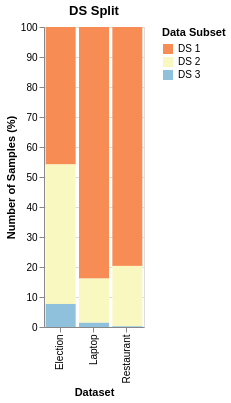
\includegraphics[scale=0.5]{images/augmentation/error_analysis/DS.png}
        }{
          \caption{Percentage of samples per \textit{DS} data subset.}
          \label{fig:aug_error_analysis_ds}
        }
        \capbtabbox{
          \begin{tabular}{|c|c|c|c|}
\hline
        & \multicolumn{3}{c|}{Data Subset} \\
\hline
Dataset &  DS 1 &  DS 2 &  DS 3 \\
\hline
Election   &  1164 &  1182 &   195 \\
\hline
Laptop     &   535 &    94 &     9 \\
\hline
Restaurant &   892 &   225 &     3 \\
\hline
\end{tabular}
        }{
          \caption{Number of samples within each \textit{DS} data subset.}
          \label{table:aug_error_analysis_ds}
        }
    \end{floatrow}
\end{figure}

The \textit{NT} split, unlike the \textit{DS} split, has a continuous number of subsets as $i$ of $NT_i$ is determined by the dataset. Figure \ref{fig:aug_error_analysis_nt_continuous} shows unsurprisingly that the Election dataset compared to the other two contain far fewer samples that only have one or two targets per text, which most likely relates to the fact that it has far fewer $DS_1$ samples. Thus, showing again that the Election dataset is likely to be a more difficult dataset, as a greater number of the samples will contain sentiment that are linked through target interaction. 
\begin{figure}[h!]
    \begin{floatrow}
        \ffigbox{
          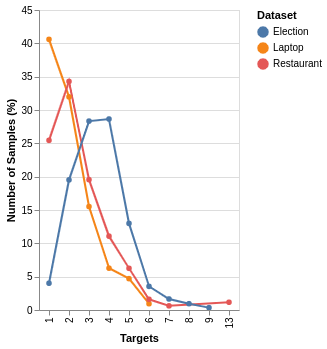
\includegraphics[scale=0.5]{images/augmentation/error_analysis/NT_continuous.png}
        }{
          \caption{Percentage of samples per $NT_i$ subset.}
          \label{fig:aug_error_analysis_nt_continuous}
        }
        \ffigbox{
          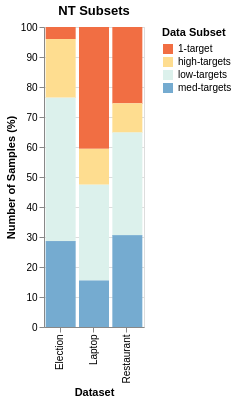
\includegraphics[scale=0.5]{images/augmentation/error_analysis/NT_discrete.png}
        }{
          \caption{Percentage of samples per \textit{NT} data subset.}
          \label{fig:aug_error_analysis_nt_discrete}
        }
    \end{floatrow}
\end{figure}
However as can be seen in figure \ref{fig:aug_error_analysis_nt_continuous} and as stated in the work suggesting this split \citep{zhang-etal-2019-aspect} some of the subsets contain very few samples, thus any analysis on these subsets can be fairly unstable. Furthermore as the dataset contain different ranges of $i$ in $NT_i$ binning the $NT$ split into four subsets will allow the datasets to be more comparable. The four subsets suggested would first be comprised of one subset where $i=1$ denoted. Then the other three subsets would be made up of low, medium, and high number of \textit{i}, where \textit{i} values for each of these subsets are based on the equal amount of samples per \textit{i}. Each of these subsets will be termed  \textit{1-target}, \textit{low-targets}, \textit{med-targets}, and \textit{high-targets} respectively. These subsets can be seen in figure \ref{fig:aug_error_analysis_nt_discrete} and table \ref{table:aug_error_analysis_nt}, along with the values of \textit{i} that each subset represents in table \ref{table:aug_error_analysis_nt_range}. The \textit{1-target} subset denotes the methods baseline performance when not having to consider target interaction, which to some extent should set the upper bound for the all other subsets. The other three subsets represent low to high likelihood of requiring target interaction knowledge to classify the samples correctly. Thus a method that can model these interactions well should perform well across all four subsets, where as a method that cannot will perform increasingly better from high \textit{i} to $i=1$.
\begin{table}[!ht]
    \centering
    \begin{tabular}{|c|c|c|c|c|}
\hline
        & \multicolumn{4}{c|}{Data Subset} \\
\hline
Dataset &  1-target &  low-targets &   med-targets &   high-targets \\
\hline
Election   &       102 &        1216    &          728 &           495 \\
\hline
Laptop     &       259 &        204     &           99 &            76 \\
\hline
Restaurant &       285 &        384    &           343 &           108 \\
\hline
\end{tabular}
    \caption{Number of samples per \textit{NT} subset.}
    \label{table:aug_error_analysis_nt}
\end{table}

\begin{table}[!ht]
    \centering
    \begin{tabular}{|c|c|c|c|c|}
\hline
        & \multicolumn{4}{c|}{Data Subset} \\
\hline
Dataset &  1-target & low-targets  & med-targets & high-targets \\
\hline
Election   &  1, 1 &     2, 3  & 4, 4  &   5, 9 \\
\hline
Laptop     &  1, 1 &    2, 2  &     3, 3 &     4, 6 \\
\hline
Restaurant &  1, 1 &    2, 2 &     3, 4 &     5, 13 \\
\hline
\end{tabular}
    \caption{Range of \textit{i} values that represent each \textit{NT} subset.}
    \label{table:aug_error_analysis_nt_range}
\end{table}

The \textit{TSSR} split as stated before in section \ref{section:error_analysis_new_splits} has a continuous number of subsets based on the dataset, of which the \textit{TSSR} subset values can range from $1$ to $0$. These \textit{TSSR} subsets can be seen in full in figure \ref{fig:aug_error_analysis_tssr_full} for each dataset. As noted before in section \ref{section:error_analysis_new_splits} the $1$ \textit{TSSR} subset is equal to the $DS_1$ subset of which this subset dominates the Laptop and Restaurant datasets. Thus for \textit{TSSR} value subsets less than $1$ the Laptop, Restaurant, and Election datasets contain $\sim20\%$, $\sim24\%$, and $\sim55\%$ of their samples respectively. Furthermore it can be seen clearly from from figure \ref{fig:aug_error_analysis_tssr_small} and \ref{fig:aug_error_analysis_tssr_full} that only the Election dataset has a large number of samples that have a \textit{TSSR} value less than or equal to $0.5$. These lower \textit{TSSR} values ($\leq 0.5$) represent the least or joint equal frequent sentiment within the text when the text comes from the $DS_2$ subset of which the majority of samples that contain more than one unique sentiment do come from the $DS_2$ for all datasets. Furthermore the lower \textit{TSSR} value subsets are going to be by far the more difficult samples to predict for, due to them containing targets that meet at least one of the two following criteria:
\begin{enumerate}
    \item The target coming from a text that contains lots of other targets but the target itself is within the least dominating sentiment class within the text.
    \item The target comes from a text that contains few targets but all targets come from a different sentiment class.
\end{enumerate}
Thus these two criteria therefore will measure the method's ability to identify target sentiment relations in a text that is dominated by other target sentiments.

\begin{figure}[!ht]
    \centering
    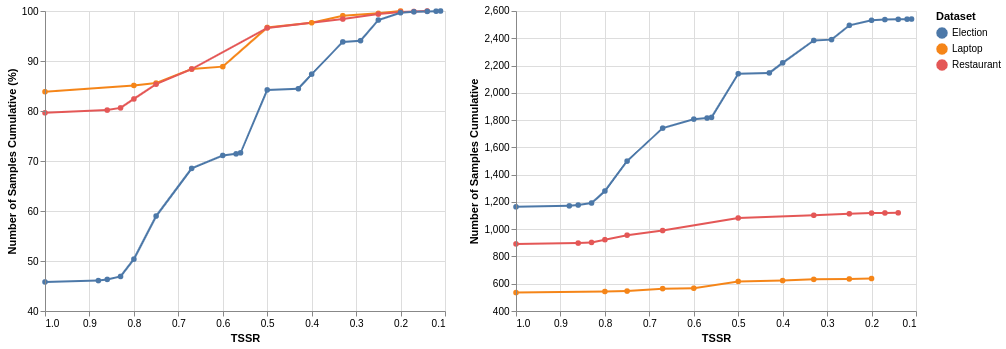
\includegraphics[scale=0.35]{images/augmentation/error_analysis/tssr_full_range.png}
    \caption{The right (left) plot shows the cumulative sample count (percentage) for decreasing values of \textit{TSSR}.}
    \label{fig:aug_error_analysis_tssr_full}
\end{figure}

\begin{figure}[!ht]
    \centering
    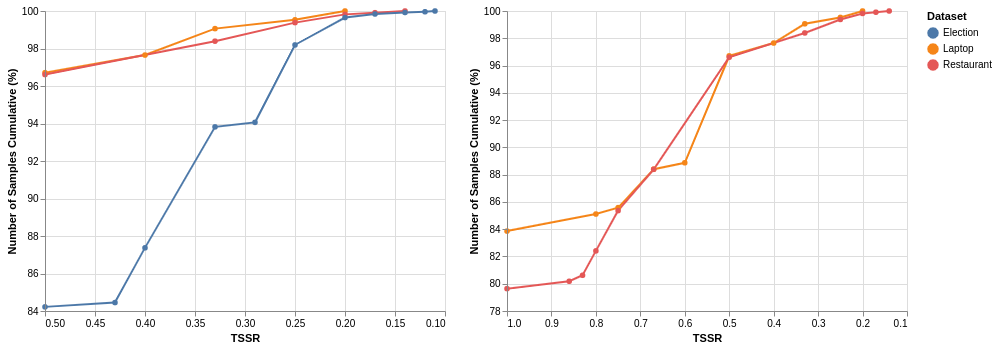
\includegraphics[scale=0.35]{images/augmentation/error_analysis/tssr_small_range.png}
    \caption{The left plot show the cumulative sample count percentage for decreasing values of \textit{TSSR} starting from $0.5$. The right plot shows the same as the left but for the full range of \textit{TSSR} values but excluding the Election dataset.}
    \label{fig:aug_error_analysis_tssr_small}
\end{figure}

As can be seen from the figures of \ref{fig:aug_error_analysis_tssr_small} and \ref{fig:aug_error_analysis_tssr_full} the \textit{TSSR} value subsets are different depending on the dataset just like the \textit{NT} split. Therefore in this thesis, the split will be contain four subsets to represent different levels of difficulty and allow the performance on the subsets to be comparable across datasets. The four subsets are the following:

\begin{enumerate}
    \item \textit{1-TSSR} contain all targets that come from a sentence that only contain that one target thus this is the same as the $NT_1$/\textit{NT 1-target} subset and \textit{ST1} subset from section \ref{section:aug_error_analysis_previous_work}. 
    \item \textit{1-multi-TSSR} contain all targets that come from a sentence that contains more than one target but they all have the same sentiment value. This is the same as the difference of the $DS_1$ subset and the $NT_1$/\textit{NT 1-target} subset, and the same as the \textit{ST2} subset from section \ref{section:aug_error_analysis_previous_work}.
    \item \textit{high-TSSR} contain all of the targets that are within the following \textit{TSSR} value range $m \le x < 1$. 
    \item \textit{low-TSSR} contain all of the targets that are within the following \textit{TSSR} value range $0 \le x < m$.
\end{enumerate}

The value for $m$ is dataset specific and is based on ensuring that the \textit{low-TSSR} values contain at least 50\% of the samples after the \textit{1-TSSR} and \textit{1-multi-TSSR} samples have been removed from the dataset. The rest of the samples are given to the \textit{high-TSSR} subset. 

The \textit{1-TSSR} subset explores the effect of having no target interaction nor complex target sentiment relation due to only having one target and one sentiment. The \textit{1-multi-TSSR} explores the effect of having target interaction with potentially easier target sentiment relation due to the targets having all of the same sentiment, thus allowing the method to get the target sentiment relation incorrect without any consequence. The \textit{high-TSSR} (\textit{low-TSSR}) measures the effect of increasing the target interaction and target sentiment relation to a smaller (larger) degree. 

The \textit{1-multi-TSSR} is expected to be the easiest subset as a method can make use of the target interaction and incorrectly inferring the correct target sentiment relationships as all targets will have the same sentiment. The next easiest subset would be the \textit{1-TSSR} due to no target interaction nor complex target sentiment relationships, however more difficult than \textit{1-multi-TSSR} as the method will have less sentiment signal within the text. Lastly the \textit{high-TSSR} and then \textit{low-TSSR} should be the most difficult subsets in that order due to target interactions and complex target-sentiment relationships. Furthermore as stated earlier in section \ref{section:error_analysis_new_splits} this split could be used to measure overfitting to most frequent sentiment within the text. Through the subsets the overfitting could be detected, if the method performs better in the \textit{1-multi-TSSR} than the \textit{1-TSSR} this could show that either the method is exploiting the frequent sentiment situation or it is better capturing the target interaction. However the difference in performance between the \textit{high-TSSR} and \textit{low-TSSR} could detect this overfitting better due to the \textit{low-TSSR} coming from the most infrequent sentiment within the texts and the \textit{high-TSSR} coming from the most frequent. Thus if the difference between the \textit{high-TSSR} and the \textit{low-TSSR} is large then most frequent sentiment overfitting is more than likely occurring.

Within figure \ref{fig:aug_error_analysis_tssr_subsets} and table \ref{table:aug_error_analysis_tssr_subsets} is the breakdown of the number of samples per \textit{TSSR} subset, table \ref{table:aug_error_analysis_tssr_subsets_range} shows the \textit{TSSR} value range for each subset\footnote{\textit{1-multi-TSSR} is not within this table as it has the same range as \textit{1-TSSR}.} (the gap in range between each subset exists because there are no samples that contain a \textit{TSSR} value in that gap). As shown in the figure and tables, the Election dataset compared to the other two contains far fewer \textit{1-TSSR} samples compared to the number of samples in \textit{1-multi-TSSR}. Furthermore, the Election dataset also contain a large \textit{high-TSSR} subset, compared to the other datasets. 

\begin{figure}[!ht]
    \centering
    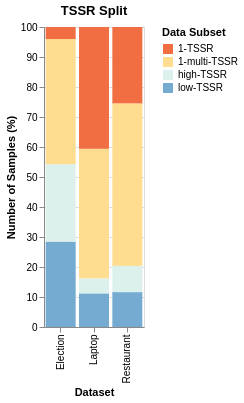
\includegraphics[scale=0.5]{images/augmentation/error_analysis/tssr_subsets.png}
    \caption{Percentage of samples per \textit{TSSR} subset.}
    \label{fig:aug_error_analysis_tssr_subsets}
\end{figure}

\begin{table}[!ht]
    \centering
    \begin{tabular}{|c|c|c|c|c|}
\hline
            &  \multicolumn{4}{c|}{Data Subset} \\
\hline 
Dataset &  1-TSSR &  1-multi-TSSR &  high-TSSR &  low-TSSR \\ 
\hline
Election   &     102 &          1062 &        656 &       721 \\
\hline  
Laptop     &     259 &           276 &         32 &        71 \\
\hline  
Restaurant &     285 &           607 &         98 &       130 \\
\hline 
\end{tabular}
    \caption{Number of samples within each \textit{TSSR} subset.}
    \label{table:aug_error_analysis_tssr_subsets}
\end{table}

\begin{table}[!ht]
    \centering
    \begin{tabular}{|c|c|c|c|}
\hline
            &  \multicolumn{3}{c|}{Data Subset} \\
\hline 
Dataset &  1-TSSR &   high-TSSR &  low-TSSR \\ 
\hline
Election   &     1, 1 &        0.88, 0.56 &       0.5, 0.11 \\
\hline  
Laptop     &     1, 1 &         0.8, 0.6 &        0.5, 0.2 \\
\hline  
Restaurant &     1, 1 &         0.86, 0.67 &       0.5, 0.14 \\
\hline 
\end{tabular}
    \caption{Range of \textit{TSSR} values for each \textit{TSSR} subset.}
    \label{table:aug_error_analysis_tssr_subsets_range}
\end{table}

To further understand the relationship between the \textit{TSSR} split and the \textit{NT} and \textit{DS} splits figure \ref{fig:aug_error_analysis_tssr_ds_nt_breakdown} shows the breakdown of each \textit{TSSR} subset by the \textit{NT} and \textit{DS} splits. As can be seen from the figure for the \textit{1-multi-TSSR} subset, the Election dataset has a more even distribution of samples that come from sentences that contain 2, 3, and 4 targets. Compared to the Restaurant and Laptop datasets where the majority of samples contain only 2 targets and then dramatically decreases as \textit{NT} increases. For all datasets the \textit{high-TSSR} subset contains relatively more samples that come from texts that contain a larger number of targets compared to the \textit{low-TSSR} subset. This is most likely due to the fact that targets with rare sentiment within the target's sentence only occur once or twice in a large \textit{NT} sentence where as the lesser rare sentiment targets occur far more often in those sentence and are counted within the \textit{high-TSSR} subset. An example of this can be thought of where the sentence contains 5 targets of which 1 comes from the positive sentiment class and the rest negative, thus the \textit{high-TSSR} will have 4 samples where as the \textit{low-TSSR} only 1 from the sentence coming from the 5 \textit{NT} subset. Unsurprisingly the majority of the limited number of $DS_3$ samples are almost all inclusively within the \textit{low-TSSR} subset for all datasets. Figure \ref{fig:aug_error_analysis_tssr_ds_nt_breakdown} also shows that the main difference between the three subsets is less about the distribution of \textit{NT} but rather the distribution of sentiment labels within a sentence. Lastly, figure \ref{fig:aug_error_analysis_tssr_ds_nt_breakdown} explains to some degree the reason why Election and Restaurant datasets have a large \textit{TSSR} value range as shown in table \ref{table:aug_error_analysis_tssr_subsets_range}, as these datasets must contain sentences that have a large number of targets as well as those sentences containing a different number of sentiments. 

\begin{figure}[!ht]
    \centering
    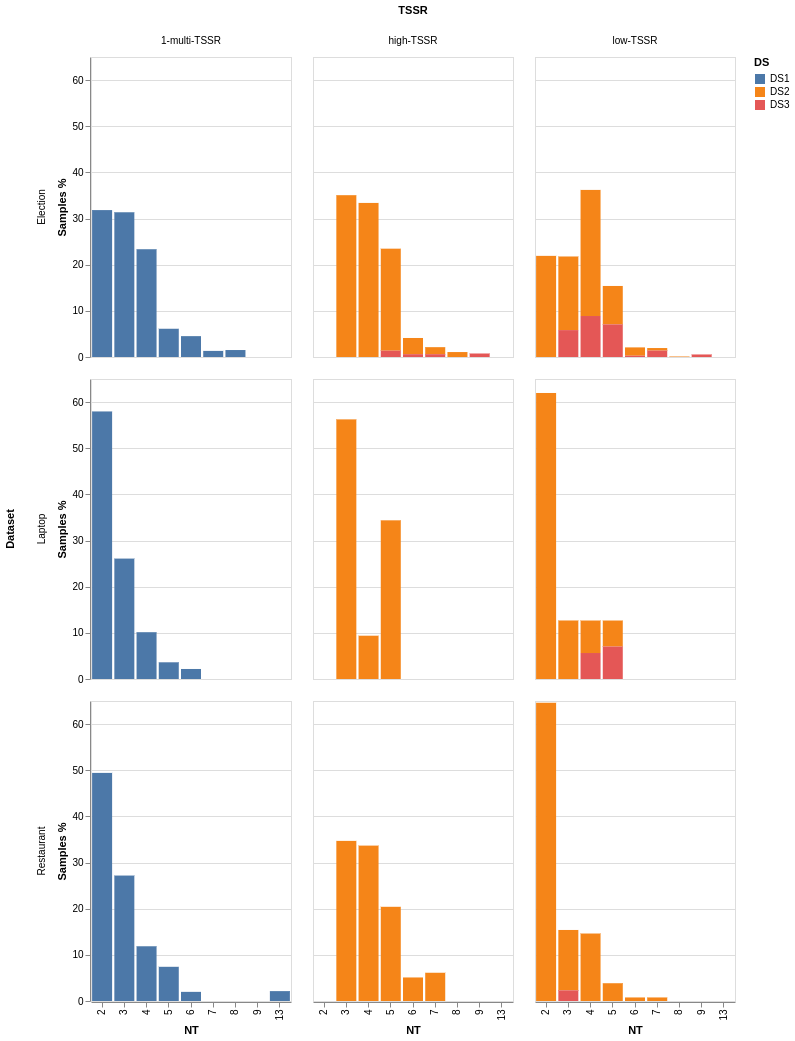
\includegraphics[scale=0.4]{images/augmentation/error_analysis/tssr_nt_ds.png}
    \caption{Percentage of samples per \textit{TSSR} subset broken down by \textit{NT} and \textit{DS} splits.}
    \label{fig:aug_error_analysis_tssr_ds_nt_breakdown}
\end{figure}

Similar to \textit{NT}, and \textit{TSSR} the \textit{n-shot} split has different values of \textit{n} based on the dataset, of which this can be best seen in figure \ref{fig:aug_n_shot_cuml}. From the left plot in figure \ref{fig:aug_n_shot_cuml} the sharpness of each curve for each dataset would appear to relate to the size of the dataset, as Laptop is the smallest and has the sharpest curve, where as Election is the largest and has the least steep curve. Furthermore, in that left plot it can be seen that both Restaurant and Election start to flatten off around 80\% and 64\% suggesting that the test dataset contains a lot of samples with targets that have been very frequently seen in the training dataset. Thus these high \textit{n} samples should be easy to classify due to the method having seen lots of samples of those targets in the training dataset. To better capture how many samples with no target in training data appear compared to those with targets that appear very often figure \ref{fig:aug_n_shot_low_med_high} contains three plots showing the low, medium, and high frequencies of \textit{n} (note that the values on the Y-axis are different). From this we can clearly see that for all datasets the largest number of samples occurs when $n=0$. Lastly it shows that both the Restaurant and Election datasets contain a lot of samples where the targets have been seen very frequently in the training dataset.

\begin{figure}[h!]
    \centering
    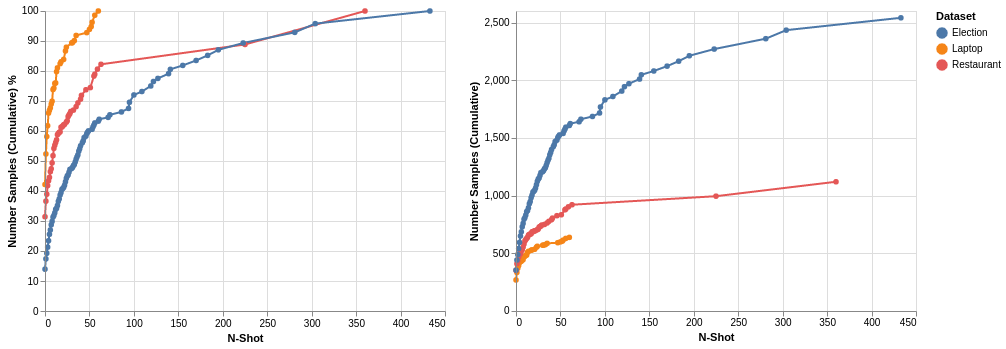
\includegraphics[scale=0.35]{images/augmentation/error_analysis/n_shot_cuml.png}
    \caption{The right (left) plot shows the cumulative sample count (percentage) for increasing values of \textit{n}.}
    \label{fig:aug_n_shot_cuml}
\end{figure}

This analysis suggests that the \textit{n-shot} split should be broken up into four different subsets rather than \textit{n} subsets, similar to the \textit{NT} split. This is suggested as a comparison of \textit{n} subsets with respect to some metric can be very unstable as some of these \textit{n} subsets can contain very few samples e.g. when $n=12$ for the Laptop dataset (see figure \ref{fig:aug_n_shot_low_med_high}). The four subsets suggested would first comprise of one subset where $n=0$ which is the \textit{UT} and \textit{zero-shot} case. Then the other three subsets would be made up of low, medium, and high number of \textit{n}, where \textit{n} values for each of these subsets are based on the equal amount of samples per \textit{n}. Each of these subsets will be termed \textit{zero-shot}, \textit{low-shot}, \textit{med-shot}, and \textit{high-shot} respectively. These subsets can be seen in figure \ref{fig:aug_error_analysis_n_shot_discrete} and table \ref{table:aug_error_analysis_n_shot}, along with the values of \textit{n} that each subset represents in table \ref{table:aug_error_analysis_n_shot_n_relation}. Lastly these subsets should allow for comparability across datasets and better analysis of the method's ability of learning a new target, as a good method should have a steady high performance across all of these subsets, whereas a method that overfits to targets would have a decreasing performance from the high to zero shot subsets.

\begin{figure}[!ht]
    \centering
    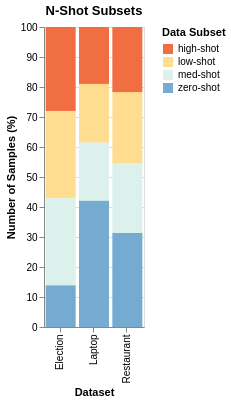
\includegraphics[scale=0.5]{images/augmentation/error_analysis/n_shot_discrete.png}
    \caption{Percentage of samples per \textit{n-shot} data subset.}
    \label{fig:aug_error_analysis_n_shot_discrete}
\end{figure}

\begin{table}[ht!]
    \centering
    \begin{tabular}{|c|c|c|c|c|}
\hline
        & \multicolumn{4}{c|}{Data Subset} \\
\hline
Dataset &   zero-shot &  low-shot &  med-shot &  high-shot \\
\hline
Election   &        354 &       740 &       736 &         711 \\
\hline
Laptop     &        269 &       125 &       123 &         121 \\
\hline
Restaurant &        352 &       267 &       258 &         243 \\ 
\hline
\end{tabular}
    \caption{Number of samples per \textit{n-shot} subset.}
    \label{table:aug_error_analysis_n_shot}
\end{table}

\begin{table}[ht!]
    \centering
    \begin{tabular}{|c|c|c|c|c|}
\hline
        & \multicolumn{4}{c|}{Data Subset} \\
\hline
Dataset &     zero-shot &   low-shot &     med-shot &  high-shot \\
\hline
Election   &  0, 0 &  1, 23 &  24, 100 &   109, 433 \\
\hline
Laptop     &    0, 0 &   1, 3 &    4, 14 &   17, 60 \\
\hline
Restaurant &    0, 0 &  1, 11 &   12, 55 &   56, 360 \\
\hline
\end{tabular}
    \caption{Range of \textit{n} values that represent each \textit{n-shot} subset.}
    \label{table:aug_error_analysis_n_shot_n_relation}
\end{table}

\begin{sidewaysfigure}[!ht]
    \centering
    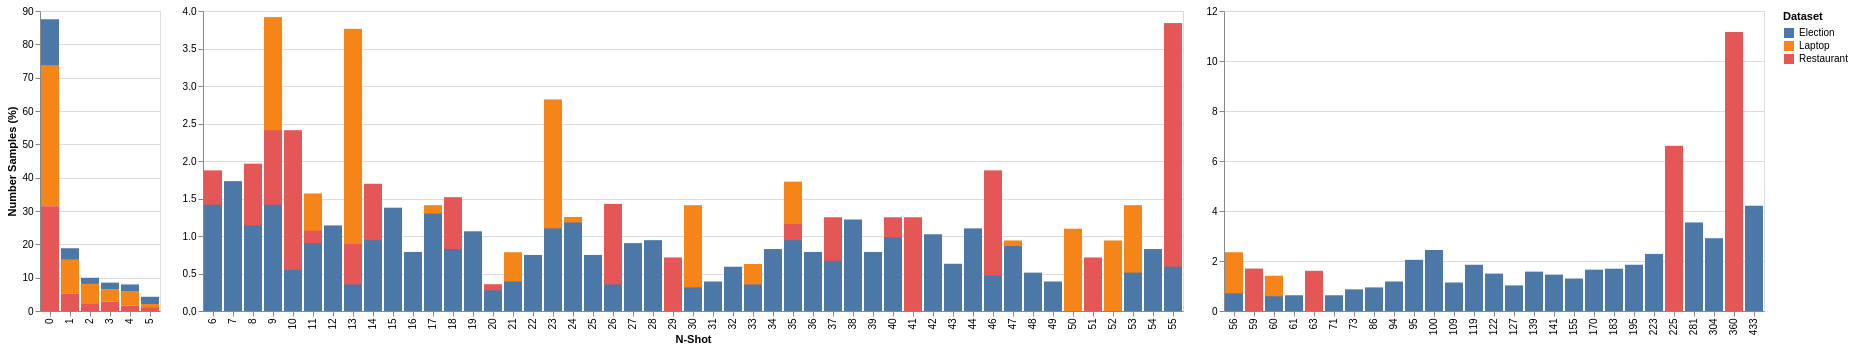
\includegraphics[scale=0.3]{images/augmentation/error_analysis/n_shot_low_med_high.png}
    \caption{Number of samples per value of \textit{n}.}
    \label{fig:aug_n_shot_low_med_high}
\end{sidewaysfigure}

The last and new split \textit{TRS} to be analysed can be best seen through figure \ref{fig:aug_error_analysis_trs} and table \ref{table:aug_error_analysis_trs}. As can be seen the \textit{UT} subset is almost the largest subset for the smallest dataset (Laptop) but relatively small subset for the largest dataset, of which this has already been seen through the \textit{zero-shot} subset. Furthermore the \textit{USKT} is the smallest subset by far across the datasets, however it still counts for at least 10\% of all data in the Laptop dataset. Based on the two global splits \textit{TRS} and \textit{n-shot} they show the importance of a method to generalise to new targets (\textit{UT} and \textit{zero-shot} cases) and new relations (\textit{USKT}) which will more likely occur in a low resource setting, which can be best seen by the size of these subsets on the Laptop dataset. 

\begin{figure}[ht!]
    \begin{floatrow}
        \ffigbox{
          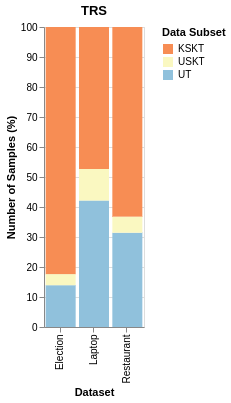
\includegraphics[scale=0.5]{images/augmentation/error_analysis/TRS.png}
        }{
          \caption{Percentage of samples per \textit{TRS} data subset.}
          \label{fig:aug_error_analysis_trs}
        }
        \capbtabbox{
          \begin{tabular}{|c|c|c|c|}
\hline
            &  \multicolumn{3}{c|}{Data Subset} \\
\hline
Dataset     &  KSKT &  USKT &  UT  \\
\hline
Election    & 2093  & 94    &  354 \\
\hline
Laptop      & 302   & 67    &  269 \\
\hline
Restaurant  & 708   & 60    &  352 \\
\hline
\end{tabular}
        }{
          \caption{Number of samples within each \textit{TRS} data subset.}
          \label{table:aug_error_analysis_trs}
        }
    \end{floatrow}
\end{figure}

\subsection{Conclusion so far}
Within this subsection the different error splits that exist within the TDSA literature have been reviewed and added too. Furthermore, each of these splits have been analysed on three major datasets showing for the first time how each dataset has different characteristics. The local splits \textit{DS}, \textit{NT}, and \textit{TSSR} show that the Election dataset contains far more unique sentiments per text, where as the Restaurant dataset contains the most targets per text. The global splits \textit{n-shot} and \textit{TRS} find that in the low resource setting a method that can generalise well to new targets and new sentiment relations would be important, which can be seen through the contrast in subset sizes between Election and Laptop datasets. Lastly, table \ref{table:aug_error_split_summary} summarises the differences in the error splits, examples for each of these splits and subsets can be found in table \ref{table:aug_error_split_examples}. Finally, a summary of all of the statistical breakdowns of each of these splits can be found in table \ref{table:aug_error_analysis_summary_stats}.

\afterpage{%
    %\clearpage% Flush earlier floats (otherwise order might not be correct)
    \thispagestyle{document}
    \begin{landscape}% Landscape page
            \centering
            \begin{longtable}{|p{0.15\linewidth}|p{0.45\linewidth}|p{0.4\linewidth}|}
\hline
Split & Description & What it measures \\
\hline
Distinct Sentiment (\textit{DS})\citep{wang-etal-2017-tdparse}. & Splits the data based on the number of unique sentiment classes within one text where $DS_i$ represents \textit{i} unique sentiment classes within a text. &  The methods ability to capture sentiment relations within the text. If the method performs well on larger values of \textit{i} the better the method is at capturing these relations. Less directly this measures the methods capability of modelling target interactions. \\
\hline
\textit{NT} \citep{zhang-etal-2019-aspect}. & Splits the data based on the number of targets within the text, where $NT_i$ split contains all the texts that have \textit{i} number of targets within it & The methods ability to model target interactions, where the larger \textit{i} is the higher the likelihood of more target interactions. For instance in example 4 from table \ref{table:aug_error_split_examples} to infer the sentiment for \textit{Dave} you need to know the sentiment towards \textit{police} and \textit{crime}.\\
\hline
\textit{TSSR} novel split. & Splits the data based on the \textit{TSSR} equation \ref{eq:aug_tssr}. The maximum value of $1$ represents a target that is within a text that contains one unique sentiment. A \textit{TSSR} value less than $1$ denotes a target that is within a text that contains at least more than one unique sentiment. A \textit{TSSR} value gets smaller based on how unique the targets sentiment is within that text. & Capturing overfitting to the most frequent sentiment within a text, which can be measured to some degree by comparing the methods High (Multi 1) \textit{TSSR} subset to the Low (1) \textit{TSSR} subset. It can also to some degree measure both target interaction and sentiment relations when the \textit{TSSR} value is less than $1$, thus a combination of both \textit{DS} and \textit{NT}.\\
\hline
\textit{ST} \citep{nguyen-shirai-2015-phrasernn}. & Splits the data into three subsets \textit{ST1} for texts that contain one target, \textit{ST2} and \textit{ST3} for texts that contain more than one target, where \textit{ST2} texts only have one unique sentiment. & The methods ability to capture sentiment relations and its interaction with other targets. \\
\hline
\textit{n-shot} \citep{yang2018multi}. & Splits the data based on the number of times the target has appeared in the training data, when $n=i$ the subset contains samples that have targets that only appear in the training data \textit{i} times. & A methods ability to generalise to unseen targets when $n=0$, as well as its capability of learning a new target. \\
\hline
\textit{TRS} novel split. & Splits the data into three subsets: 1. \textit{Unknown Targets}(\textit{UT}) when the target has never been seen in the training data, 2. \textit{Unknown Sentiment Known Target}(\textit{USKT}) when the target has been seen in the training data but not with the same sentiment class, and 3. \textit{Known Sentiment Known Target}(\textit{KSKT}) when the target has been seen in the training data with the same sentiment class. NOTE \textit{UT} is equal to \textit{n-shot} when $n=0$. & A methods ability to generalise to unseen targets \textit{UT} split, and unknown sentiment relations \textit{USKT} split, where the \textit{KSKT} split can be seen as the methods upper limit for the former two subsets performance. \\
\hline
\caption{Summary of the different error splits.}
\label{table:aug_error_split_summary}
\end{longtable}
    \end{landscape}
    \clearpage% Flush page
}

\begin{table}[!ht]
    \centering
    \begin{tabular}{|p{7cm}|p{3cm}|}
\hline
Sample & Error subsets for each target \\
\hline
\multicolumn{2}{|c|}{Examples in training data} \\ 
\hline
\multicolumn{2}{|c|}{Example 1} \\
\hline
\textcolor{green}{Conservatives}\textsubscript{1} cut the \textcolor{green}{police}\textsubscript{2} budget and this cut \textcolor{red}{crime}\textsubscript{3}! Maybe not... \#spin \#BattleForNumber10 & All targets - $DS_2$, \textit{ST3}, $NT_3$. Target $1$ and $2$ - \textit{TSSR} value of $\frac{2}{3}$. Target $3$ - \textit{TSSR} value $\frac{1}{3}$. \\
\hline
\multicolumn{2}{|c|}{Example 2} \\
\hline
Absolutely - \textcolor{red}{taxation}\textsubscript{1} is the problem \#bbcqt & All targets - $DS_1$, \textit{ST1}, $NT_1$, \textit{TSSR} value $1$. \\
\hline
\multicolumn{2}{|c|}{Example 3} \\
\hline
Let the debate begin need a leader with tolerance for \textcolor{blue}{immigrants}\textsubscript{1}/\textcolor{blue}{refugees}\textsubscript{2} \#BattleForNumber10 & All targets - $DS_1$, \textit{ST2}, $NT_2$, \textit{TSSR} value $1$. \\
\hline
\multicolumn{2}{|c|}{Examples in test data} \\ 
\hline
\multicolumn{2}{|c|}{Example 4} \\
\hline
20\% less \textcolor{red}{police}\textsubscript{1} equals 20\% less \textcolor{red}{crime}\textsubscript{2}...wow \textcolor{red}{Dave}\textsubscript{3}'s a genius... \#BattleForNumber10 & All targets - $DS_1$, \textit{ST1}, $NT_3$, \textit{TSSR} value $1$. Target $1$ - $1$-shot, \textit{USKT}, Target 2 - $1$-shot, \textit{KSKT}, Target 3 - $0$-shot, \textit{UT}. \\
\hline
\multicolumn{2}{|c|}{Blue = positive, Green = neutral, and Red = negative sentiment.} \\
\hline
\end{tabular}
    \caption{Examples of TDSA samples split into training and test datasets, where each example states the error split that the target will be put within. All examples have come from the Election Twitter dataset \citep{wang-etal-2017-tdparse}.}
    \label{table:aug_error_split_examples}
\end{table}

\begin{table}[!ht]
    \centering
    \begin{tabular}{|c|c|c|c|c|}
\hline
    &    & \multicolumn{3}{c|}{Dataset} \\
\hline
Data Split & Data Subset &  Election &  Laptop &  Restaurant \\
\hline
\multirow{3}{*}{$DS_i$} & $DS_1$ &      45.8\% &    83.9\% &        79.6\% \\
 & $DS_2$ &      46.5\% &    14.7\% &        20.1\% \\
 & $DS_3$ &       7.7\% &     1.4\% &         0.3\% \\
\hline
 \multirow{4}{*}{\textit{NT}} & \textit{1-target} &       4.0\% &    40.6\% &        25.4\% \\
 & \textit{low-targets} &      47.9\% &    32.0\% &        34.3\% \\
 & \textit{med-targets} &      28.7\% &    15.5\% &        30.6\% \\
 & \textit{high-targets} &      19.5\% &    11.9\% &         9.6\% \\
\hline
 \multirow{4}{*}{\textit{TSSR}} & \textit{1-TSSR} &       4.0\% &    40.6\% &        25.4\% \\
 & \textit{1-multi-TSSR} &      41.8\% &    43.3\% &        54.2\% \\
 & \textit{high-TSSR} &      25.8\% &    5.0\% &         8.8\% \\
 & \textit{low-TSSR} &      28.4\% &    11.1\% &        11.6\% \\
 \hline
 \multirow{3}{*}{\textit{TRS}} & \textit{KTKS} &      82.4\% &    47.3\% &        63.2\% \\
 & \textit{USKT} &       3.7\% &    10.5\% &         5.4\% \\
 & \textit{UT} &      13.9\% &    42.2\% &        31.4\% \\
\hline
 \multirow{4}{*}{\textit{n-shot}} & \textit{zero-shot} &      13.9\% &    42.2\% &        31.4\% \\
 & \textit{low-shot} &      29.1\% &    19.6\% &        23.8\% \\
 & \textit{med-shot} &      29.0\% &    19.3\% &        23.0\% \\
 & \textit{high-shot} &      28.0\% &    19.0\% &        21.7\% \\
\hline
 \multicolumn{2}{|c|}{Total Samples}           &    2541 &  638 &      1120 \\
\hline
 \end{tabular}
    \caption{Summary statistics of all splits}
    \label{table:aug_error_analysis_summary_stats}
\end{table}

\section{Method Performance on the Error Splits}
\subsection{Introduction}
\label{section:aug_method_performance_intro}
In this sub-section the performance of the following four NN based methods will be analysed across the five different error splits stated in last section \ref{section:aug_error_analysis}. The results from these experiments will be used to further analyse what the error splits show as well as create multiple baselines for these splits. The four different methods are the following: 
\begin{enumerate}
    \item \textit{CNN} -- The sentence level CNN from \citet{kim-2014-convolutional} that encodes the context/sentence and does not take into account the target.
    \item \textit{TDLSTM} \citep{tang-etal-2016-effective} -- A LSTM that encodes the target by ensuring the target word(s) are always the last word(s) fed to the LSTM from the context/sentence. Thus a position based method where the position is encoded through the NN architecture.
    \item \textit{IAN} \citep{ma2017interactive} -- Encodes the target into the context via attention.
    \item \textit{Att-AE} -- A model that is the same as the \textit{AE} model from \citet{wang-etal-2016-attention} but with an attention layer after the LSTM enocder. This model is also the same as the inter-aspect model (from now on called \textit{Inter-AE}) from \citet{hazarika-etal-2018-modeling} but without the LSTM aspect encoder (phase 2 in figure 1) that models other targets from the same context/sentence.  
\end{enumerate}
Thus to summarise the differences in the TDSA methods (last three methods from above); \textit{TDLSTM} encodes the position of targets through its architecture, \textit{IAN} encodes the target into the context via attention and also encodes the context into the target through attention, and \textit{Att-AE} encodes the target into the context through concatenation of the target vector onto each word vector within the context before the LSTM encoder. The \textit{Att-AE} does perform attention over the context but unlike \textit{IAN} does not explicitly model the target in the attention of the context nor does it perform attention over the target word(s)\footnote{For the detailed reader, the \textit{IAN's} attention can be denoted as \textit{general} where as \textit{Att-AE} would be \textit{concat} based on the notation from section 3.1. of \citet{luong-etal-2015-effective}.}.

Furthermore as stated in the introduction section \ref{section:aug_introduction}, the TDSA methods will be enhanced with three different developments; 1. position-encoding, 2. inter-target encoding, and 3. CWR. From the three methods, only \textit{IAN} and \textit{Att-AE} will be enhanced with position-encoding as \textit{TDLSTM} already has the target position somewhat encoded into its NN architecture. Each of these enhancements will be tested against their standard/base model with respect to the error analysis splits. The quantitative results from these error analysis splits will be compared to the original qualitative justifications for these developments from the respective papers.

The reason why \textit{Att-AE} is neither exactly \textit{AE} \citep{wang-etal-2016-attention} nor \textit{Inter-AE} \citep{hazarika-etal-2018-modeling} is because we did not want to add inter-target encoding to the baselines models as later on in this chapter all models are going to have inter-target encoding added. Furthermore as the model will have inter-target encoding added it will convert \textit{Att-AE} to \textit{Inter-AE} thus making it a standard model from prior literature.

Due to having a non-target method \textit{CNN} all of the TDSA methods have a baseline to compare against. Furthermore as all experiments will contain results from at least two TDSA methods the comparisons between the base model and the enhanced should be more robust and to a larger extent the results should generalise to different TDSA NN architectures. In the following sections the thesis will:
\begin{enumerate}
    \item State the experimental setup of all experiments within this section (section \ref{section:aug_experimental_setup}).
    \item Explore the differences in performance on the error splits across the methods (section \ref{section:aug_baseline}).
    \item Evaluate the error split across three different model enhancements position encoding (section \ref{section:aug_position_encoding}), inter target encoding (section \ref{section:aug_inter_target_encoding}), and CWR (section \ref{section:aug_cwr}).
\end{enumerate}

\subsection{Experimental Setup}
\label{section:aug_experimental_setup}
As stated in the introductory section of this chapter \ref{section:aug_introduction}, the three datasets that are used throughout this chapter are the Election, Laptop and Restaurant datasets. However unlike the error analysis section \ref{section:aug_error_analysis}, the standard training split for each of the datasets will be further randomly split into a new training and an additional validation split, of which the size of these splits can be seen in table \ref{table:aug_methods_performance_split_breakdown}. The validation set is required so that the early stopping can be used for all of the NN methods. Furthermore, the validation set would usually be used for more hyper-parameter tuning e.g. finding the best learning rate etc. but due to compute time this is not the case. Instead we selected the most common hyper-parameters from the literature as detailed in table \ref{table:aug_methods_performance_default_hyperparameters}, it will be stated explicitly within this chapter if these hyperparameters are not used. One default hyperparameter of note is the embedding, of which the 840 billion token 300 dimensional GloVe vector \citep{pennington-etal-2014-glove} (from now on called \textit{GloVe} and is called that in table \ref{table:aug_methods_performance_default_hyperparameters}) was chosen, as it is the most common default embedding in the TDSA literature. Lastly all results reported in this section will be results on the test set and all validation results will be reported in the appendix for reproducibility reasons \citep{dodge-etal-2019-show}. However if there is a large difference between the validation and test results this will be mentioned explicitly in this section.

\begin{table}[ht!]
    \centering
    \begin{tabular}{|c|c|c|c|c|}
\hline
        & \multicolumn{4}{c|}{Data Split} \\
\hline
Dataset &          Train &     Validation &           Test &  Total \\
\hline
Election   &  6811 (57.24\%) &  2547 (21.41\%) &  2541 (21.35\%) &  11899 \\
\hline
Laptop     &  1661 (56.29\%) &   652 (22.09\%) &   638 (21.62\%) &   2951 \\
\hline
Restaurant &  2490 (52.73\%) &  1112 (23.55\%) &  1120 (23.72\%) &   4722 \\
\hline
\end{tabular}
    \caption{Number of samples.}
    \label{table:aug_methods_performance_split_breakdown}
\end{table}

Due to the splitting of the training dataset, the error analysis split statistics in section \ref{section:aug_error_analysis} will not be identical for the global error splits (\textit{n-shot} and \textit{TRS}) between the train/test and train/validation as they rely on a comparison of train and validation/test. Even though they will not be identical they are relatively similar as shown by table \ref{table:aug_methods_performance_global_error_diff}. Furthermore as the local splits (\textit{DS}, \textit{NT}, and \textit{TSSR}) are only reported for the test set, table \ref{table:aug_methods_performance_local_error_diff} shows them for the validation and test set showing that they are again relatively similar, thus results should be comparable between validation and test sets.

Furthermore for all of the experiments performed in this chapter each model will have trained/ran on the respective data eight times. Thus allowing for the random seed problem that is known in NN methods within NLP \citep{reimers-gurevych-2017-reporting} and to be able to perform statistical significance tests that take into account this problem \citep{reimers2018comparing}. \citet{reimers2018comparing} has shown that by using a minimum of eight runs two models can be compared with a confidence level of 99\% which is equivalent to $p \leq 0.01$ no matter if the scores from those runs comes from a non-normal distribution. The two scoring metrics commonly used in TDSA and will be used in this chapter are accuracy and macro F1, of which only accuracy can be assumed to produce scores originating from a normal distribution and thus can use the more powerful parametric tests \citep{dror-etal-2018-hitchhikers}. Therefore following \citet{reimers2018comparing} for the accuracy scores the significance test used will be the Welch's t-test (parametric test) \citep{welch1947generalization} and for macro F1 the Wilcoxon signed-rank test (non-parametric test) \citep{wilcoxon1992individual}. When comparing two models using these statistical tests for each test the one-tailed version of it will be used as in these experiments the requirement is only to know if one model is better than another. Before going into the details of comparing two models across multiple variables, we first need to define what the differences are between a method and a model. A method is the general NN architecture where as the model is the concrete configuration of that method. Thus two models can be different but use the same method, for example the difference would be the word vectors that the two models use. When comparing two models the value of $\alpha$ in $p \leq \alpha$ is used to define the number of type 1 errors in the statistical test. However when comparing two models across multiple variables and therefore multiple significance tests if the number of times a test is defined as significant are simply counted the number of type 1 errors in the tests will increase \citep{dror-etal-2017-replicability}. Thus simply counting the number of times a test is significant cannot be used without further introducing type 1 errors. To bound these type 1 errors across multiple tests requires a correction mechanism of which \citet{dror-etal-2017-replicability} recommends Bonferroni (Fisher) when the variables are dependent (independent), where Fisher is the more powerful version. In this chapter, Bonferroni will be used where appropriate as in none of our cases can independence be assumed.

\subsection{Baseline Results\footnote{Notebook associated to these results can be found here: \url{https://bit.ly/37GUObF}.}}
\label{section:aug_baseline}
The baseline results use the four different methods stated in section \ref{section:aug_method_performance_intro} as is without any changes to their respective NN architectures. These results will be explored to see whether the intuition behind the error splits as stated in section \ref{section:aug_analysing_the_splits} is to a degree true. 

For clarification, the sentence/text level \textit{CNN} method is trained differently to the TDSA methods due to the fact that it does not model the target within the sentence. Thus instead of training the \textit{CNN} method with potentially the same sentence multiple times with potentially multiple different sentiments as is the case with TDSA datasets, the TDSA dataset is converted to a text level dataset. To convert from TDSA to a text dataset each text/sentence can only contain one sentiment, from this two options are plausible; 1. only uses texts that contain one unique sentiment ($DS_1$ dataset), or 2. use the majority sentiment from the text. These two options were compared of which the detailed results can be found in appendix \ref{section:appendix_cnn_tdsa_baseline}, of which it was found that the second/later option performed best on 2 (3) of the 3 datasets for the accuracy (macro f1) metric across both validation and test splits. This experiment of comparing the two options of training a text classifier on TDSA data was required as prior works that have shown results for text classifiers but never explain how they were trained \citep{tang-etal-2016-aspect,wang-etal-2016-attention,he-etal-2018-exploiting,jiang-etal-2019-challenge}. For a stronger text classifier baseline one could consider pre-training the text classifier from large sources of annotated data such as Yelp reviews \citep{tang-etal-2015-learning}, Amazon reviews \citep{mcauley2015image,he2016ups}, or Tweets using distant supervision \citep{go2009twitter} for the Restaurant, Laptop, and Election datasets respectively and then fine tune them on the respective TDSA dataset. However this stronger baseline is not considered in this work as we are not looking at transfer learning from other sources of sentiment, but this has been shown beneficial for TDSA methods \citep{he-etal-2018-exploiting}.  

Figure \ref{fig:aug_baseline_overall_scores} shows the results of the baselines models across both the validation and test splits with the associated tables \ref{table:aug_methods_baseline_tdsa_metrics_validation} and \ref{table:aug_methods_baseline_tdsa_metrics_test} in appendix \ref{section:appendix_tdsa_baseline_metrics}. From these results it can be seen that the \textit{CNN} text classification baseline is indeed a strong baseline for the Laptop and Restaurant datasets that the TDSA methods find difficult to beat. 

\begin{figure}[ht!]
    \centering
    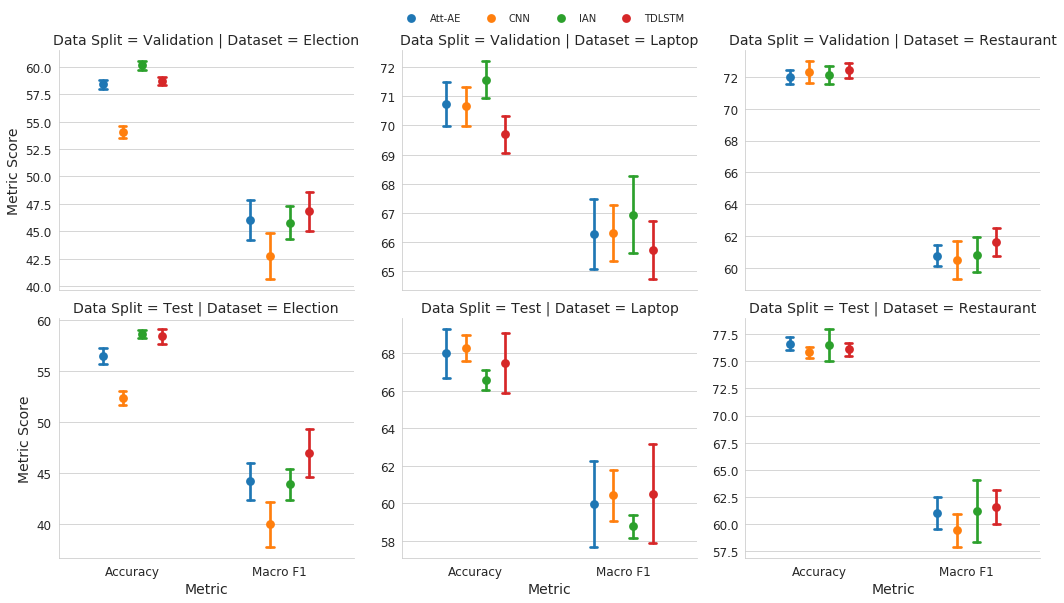
\includegraphics[scale=0.3]{images/augmentation/methods_performance/baseline/baseline_overall_scores.png}
    \caption{The mean and standard deviation error bars from running each model 8 times.}
    \label{fig:aug_baseline_overall_scores}
\end{figure}

Figure \ref{fig:aug_baseline_replication_scores} compares the single run performance of the original TDSA models scores from their associated papers to the distribution of eight accuracy scores from our replicated TDSA methods\footnote{Accuracy metric was the only metric reported in all of the original TDSA method papers and none of them reported on the Election dataset.}. As can be seen from figure \ref{fig:aug_baseline_replication_scores} the models original score are within the distribution of scores from the replicated models apart from \textit{IAN} where the original models performance is a lot higher especially for the Laptop dataset. \textit{IAN's} performance difference is most likely due to the fact that the replicated version uses a different optimiser, ADAM, instead of SGD with momentum, this design choice was made so that all models used the same optimiser. Even though it would be good to optimise the performance of the \textit{IAN} model so that it produces scores similar to the original doing so in a fair manner would mean hyperparameter tuning the other models as well \citep{dodge-etal-2019-show}, which would start becoming computationally expensive. Thus in this thesis it is accepted that the \textit{IAN} model has not been replicated to the same performance as the original paper reports.

\begin{figure}[ht!]
    \centering
    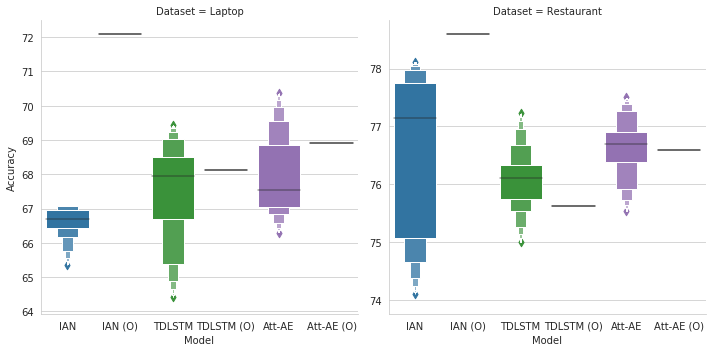
\includegraphics[scale=0.32]{images/augmentation/methods_performance/baseline/replication_experiment_baseline.png}
    \caption{Distribution of all scores and the line represents the mean value, of which for the original models this line represents their only reported score. Model names with a \textit{(O)} represent the score reported in the original models paper.}
    \label{fig:aug_baseline_replication_scores}
\end{figure}

Given that at least two of the three TDSA models are replicated to the same level as the original paper and in all three original papers they compare these models or in the case of \textit{Att-AE}\footnote{For the \textit{Att-AE} the compared original version is the \textit{AE} model from \citet{wang-etal-2016-attention}.} a similar model to a text classification baseline and state that the models are superior. This thesis shows for the first time that not all TDSA models are statistically significantly better than a text classifier as shown by table \ref{tab:augmentation_baseline_tdsa_text_classifier_p_values}. Furthermore at the $95\%$ confidence level none of the TDSA methods are significant on the Laptop test split no matter what the metric is. This shows that potentially hyperparameter tuning is very important to get the most out of the TDSA models. More likely the reason for the text classifier's strong performance on the Laptop and Restaurant dataset compared to that Election is that these dataset contain a large quantity of $DS_1$ samples (see figure \ref{fig:aug_error_analysis_ds}), of which it is shown later in this section in figure \ref{fig:aug_baseline_test_error_subset} that the text classifier does at least as good if not better than the TDSA models on the $DS_1$ subset in the Laptop and Restaurant datasets. This further shows that the overall metrics tell us very little in what the difference is between a text classifier model and the TDSA models.  
%\citet{jiang-etal-2019-challenge} concluded as well for the Restaurant dataset\footnote{\citet{jiang-etal-2019-challenge} did not perform any significance tests between existing TDSA methods and the text classifier baselines.} that the text classifier good performance was due to the large quantity of text. Furthermore as shown 



\begin{table}[ht!]
    \centering
    \begin{tabular}{|c|c|c|c|c|c|}       
\hline
&            &  & \multicolumn{3}{c|}{Dataset} \\
\hline
Model & Split & Metric &      Election         &    Laptop       &  Restaurant           \\
\hline
Att-AE & \multirow{2}{*}{Test} & Accuracy &  \textbf{2.14e-08} &  0.68 &    \textbf{0.01} \\
&            & Macro F1 &  \textbf{7.86e-04} &  0.67 &    \textbf{0.03} \\
& \multirow{2}{*}{Validation} & Accuracy &  \textbf{2.57e-10} &  0.40 &    0.84 \\
&            & Macro F1 &  \textbf{3.76e-03} &  0.52 &    0.31 \\
\hline
IAN & \multirow{2}{*}{Test} & Accuracy &  \textbf{2.21e-10} &  0.99 &    0.14 \\
&            & Macro F1 &  \textbf{1.02e-03} &  0.99 &    0.08 \\
& \multirow{2}{*}{Validation} & Accuracy &  \textbf{3.98e-12} &  \textbf{0.01} &    0.69 \\
&            & Macro F1 &  \textbf{3.96e-03} &  0.16 &    0.30 \\
\hline
TDLSTM & \multirow{2}{*}{Test} & Accuracy &  \textbf{1.29e-10} &  0.87 &    0.19 \\
&            & Macro F1 &  \textbf{2.53e-05} &  0.46 &    \textbf{0.01} \\       
& \multirow{2}{*}{Validation} & Accuracy &  \textbf{1.26e-10} &  0.99 &    0.36 \\
&            & Macro F1 &  \textbf{8.07e-04} &  0.85 &    \textbf{0.03} \\
\hline
\end{tabular}
    \caption{The P-values for each model where the null hypothesis is that each model performs as well as a \textit{CNN} text classifier. The P-Values in bold are those $\leq 0.05$.}
    \label{tab:augmentation_baseline_tdsa_text_classifier_p_values}
\end{table}

The performance of all of the models across all datasets for each split and their associated subsets can be seen in \ref{fig:aug_baseline_test_error_subset} (figure \ref{fig:aug_baseline_validation_error_subset} shows the validation split results). The figures that contain subset performance results will not contain results for the $DS_3$ subset for the Laptop and Restaurant datasets, this is due the subset containing very few samples as highlighted in the previous subsection \ref{section:aug_analysing_the_splits}. The error split results for the test (validation) split are better highlighted in figure \ref{fig:aug_baseline_test_error_diff_subset} (figure \ref{fig:aug_baseline_validation_error_diff_subset}) where the accuracy on the whole datasets (overall accuracy) is subtracted from the error subset accuracies. These figures can thus evaluate the error splits that were discussed and created within this section. In the list below the results will be analysed by error split:

\begin{itemize}
    \item \textit{DS} split, as expected, increases in difficulty as the number of unique sentiments in the text increases, thus showing that target sentiment relation to be a difficult task for the model to perform. Furthermore it can be seen that on average the \textit{TDLSTM} model performs consistently well on the $DS_2$ and $DS_3$ subsets compared to the other models.
    \item \textit{NT} split does not have a consistent affect on the performance of the models, this was also found in one of the original papers \citep{zhang-etal-2019-aspect}. One would expect texts that contain a lot of targets to be more difficult and at times it is as shown by the Restaurant dataset. However on the other two datasets this is not the case. Furthermore the performance across the subsets can differ between datasets splits e.g. the performance of all models on the \textit{med-targets} subset on the Election dataset is worse than \textit{high-targets} for all models on the test split but on the validation figure \ref{fig:aug_baseline_validation_error_diff_subset} the opposite is true. This would suggest that even though theoretically a text with more targets should be more difficult for a model to classify, due to the complexities of matching targets to their respective sentiments \citep{zhang-etal-2019-aspect}, this is not the case. Thus later in this section analysis is conducted to investigate what other factors are influencing the change in performance within the \textit{NT} split. However for now it can be concluded that \textit{NT} cannot effectively evaluate the target interaction as no consistent trend can be found in this split.
    \item \textit{TSSR} As expected the \textit{1-Multi} subset is by far the easiest subset to classify suggesting that the models are exploiting the fact that all targets have the same sentiment. The \textit{1} subset tends to perform the next best with the \textit{high} subset at times quite close if not the same. A reason for the \textit{high} subset to have such high performance across the models could be due to the models overfitting to the most frequent sentiment class in the text, as suggested in section \ref{section:aug_error_analysis}. As expected the \textit{low} subset is by far the worse across all datasets and models and in some cases harder to classify than samples within $DS_2$ and $DS_3$. Only on the Laptop test split is the \textit{high} scores similar to the \textit{low}, of which this might be due to the lack of samples for the \textit{high} subset (5\% of the dataset) compared to the (11.1\% of the dataset) in the \textit{low} subset, which is also suggested by the large error bars. Furthermore the sentiment overfitting which this split is suppose to measure does show to some extent where the TDSA model, \textit{TDLSTM}, that performs consistently better or at least as good in the $DS_2$ and $DS_3$ subsets tends to have a smaller difference between subset \textit{1-Multi} and \textit{1}, and is consistently a lot higher than the text classifier on the \textit{low} subset. However this split does not measure sentiment overfitting explicitly very well without the text classification baseline and the \textit{DS} split. For example without \textit{DS} and the text classification baseline it would be impossible to know that the \textit{TDLSTM} is performing target sentiment relation well on the laptop dataset as the $DS_2$ subset performance could be high due to \textit{TDLSTM} predicting the most frequent sentiment class. This cannot be the case as the performance of \textit{TDLSTM} on the \textit{high} and \textit{low} \textit{TSSR} subsets are both above the text classification model unlike the other two TDSA models. Though this is a rather loose way of measuring sentiment overfitting and is not the way that was stated in the previous subsection \ref{section:aug_analysing_the_splits}. In the previous  subsection \ref{section:aug_analysing_the_splits} the difference between the \textit{high} and \textit{low} subsets was hypothesised to indicate sentiment overfitting, but as can be seen from the figures \textit{TDLSTM} that is suppose to not be overfitting as much as the other TDSA models does indeed contain a low difference between \textit{high} and \textit{low} on the Laptop dataset, but so does \textit{IAN} thus makes the hypothesis less likely to be true. Therefore to conclude on the \textit{TSSR} split, it cannot measure sentiment overfitting nor would it be able to measure target interaction as suggested in \ref{section:aug_analysing_the_splits} either as it would be impossible to know if it was target interaction or sentiment overfitting. However there are clear signs that the subsets measure to some degree target sentiment relation as the score of subsets \textit{1}, \textit{high}, and \textit{low} are similar in order to subsets $DS_1$, $DS_2$, and $DS_3$ respectively and these subsets co-occur frequently as shown in figure \ref{fig:aug_error_analysis_tssr_ds_nt_breakdown}. Thus after this subsection the \textit{TSSR} split will no longer be used. 
    \item \textit{TSR} again the finding is expected where the \textit{USKT} is by far the most difficult subset. The \textit{UT} is more difficult in general than the \textit{KSKT} but with a much smaller margin. This finding is therefore in line with the relation extraction literature where unknown entities are easier to predict than unknown relations \citep{levy-etal-2017-zero,abdou-etal-2019-x}. Within the validation results for the Election dataset the margin between \textit{UT} and \textit{KTKS} is very small. This very much suggests that the models do require a certain amount of supervision for all targets in all sentiment classes or else they bias the target more towards one sentiment class than another. This type of bias can be very harmful as shown by the \textit{USKT}. This could suggest a reason why the margin between \textit{UT} and \textit{KSKT} is so small as some of the \textit{KSKT} targets might not occur in enough samples within a sentiment class. Furthermore the \textit{KSKT} subset can be seen as the upper limit for the other two subsets as it can be seen as the data rich subset.
    \item \textit{n-shot} the expected result can be clearly seen in all the datasets within the test split but less so within the validation split. Where the expectation is that the greater \textit{n} is the easier the subset will be. Within the validation split the Election and to some extent Restaurant datasets are the major outliers, where no matter what the subset is, the scores are almost all the same. A reason for this could be that the validation split is used in early stopping therefore some information is leaked to the model. As both the \textit{n-shot} and \textit{TSR} splits measure a models generalisation to new targets, from the results shown it would appear that \textit{TSR} does this more explicitly. The \textit{TSR} split unlike the \textit{n-shot} models both the unseen targets and unseen relations, of which modelling both has been shown through \textit{TSR} to be crucial. This finding creates another possible explanation why the \textit{n-shot} subsets do not show a positive correlation between \textit{n} and the metric score. Furthermore the \textit{TSR KSKT} subset is always the best performing subset within the split unlike the \textit{high} in the \textit{n-shot}. Thus for exploring a models ability to generalise to unknown targets and unknown sentiment relations \textit{TSR} is recommended compared to \textit{n-shot}. Thus like the \textit{TSSR} split the \textit{n-shot} will not be used after this subsection.
\end{itemize}
Generally the results from figure \ref{fig:aug_baseline_test_error_subset} (validation dataset figure \ref{fig:aug_baseline_validation_error_subset}) show that the \textit{DS}, \textit{TSSR}, and \textit{TSR} splits contain the most difficult subsets. The TDSA models perform a lot better on the $DS_2$ subset on the Election datasets compared to the Laptop and Restaurant datasets. This could be due to the Election dataset containing far more $DS_2$ samples relative to it's overall size compared to Laptop and Restaurant datasets (see figure \ref{fig:aug_error_analysis_ds}). This may suggest that ways to improve the models performance on the $DS_2$ and potentially $DS_3$ subsets could be by training the models on more of these samples and thus improving the target sentiment relation modelling. However this could have a negative affect on the performance in the $DS_1$ subset. Also how to generate more $DS_2$ and $DS_3$ samples could also be a difficult and interesting challenge.

From figure \ref{fig:aug_baseline_test_error_subset} (validation dataset figure \ref{fig:aug_baseline_validation_error_subset}) the text classification model has a few unexpected findings. The \textit{TSR}, and \textit{n-shot} splits do not explicitly probe a models capability to model the target sentiment relationship rather how well a model generalises to new targets or less seen targets and unknown sentiment classes for known targets. These probes thus do not explicitly require target information, for example in the \textit{DS} split for the $DS_2$ subset without modelling the target it is impossible to get all the samples correct, this is not directly true for the subsets in the \textit{n-shot} and \textit{TSR}. However as can be seen from the results the text classification model does not perform equally well across all subsets in the \textit{n-shot} and \textit{TSR} splits, this suggest that either the text classification model does use the target to influence the sentiment prediction, or these subsets correlate with other dataset factors, for example \textit{zero-shot} subset has far fewer samples that belong to the $DS_2$ subset than the \textit{high-shot} subset. These issues are not explored any further but should be looked at in the future.

\begin{figure}[ht!]
    \centering
    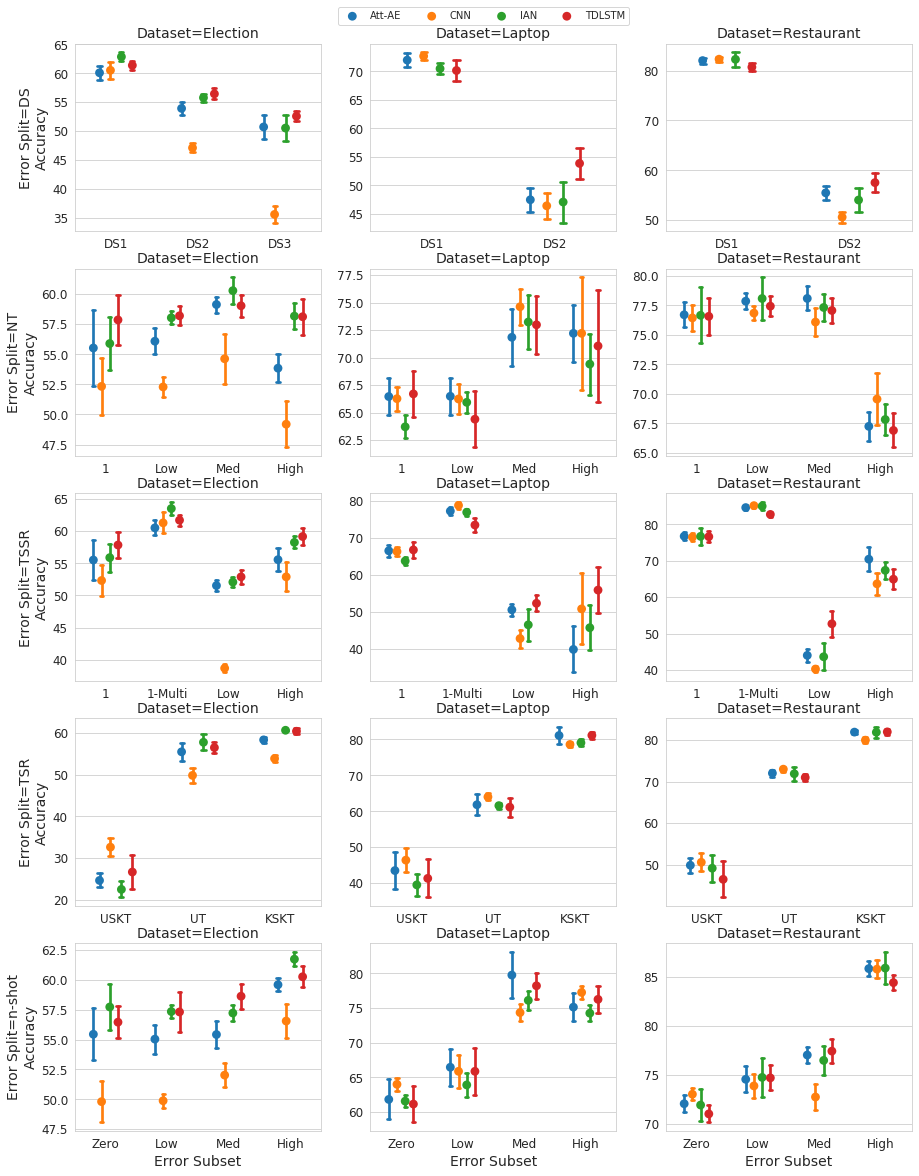
\includegraphics[scale=0.3]{images/augmentation/methods_performance/baseline/test_error_subsets.png}
    \caption{The mean and standard deviation error bars for each error subset within all of the error splits on the test split across all datasets.}
    \label{fig:aug_baseline_test_error_subset}
\end{figure}

\begin{figure}[ht!]
    \centering
    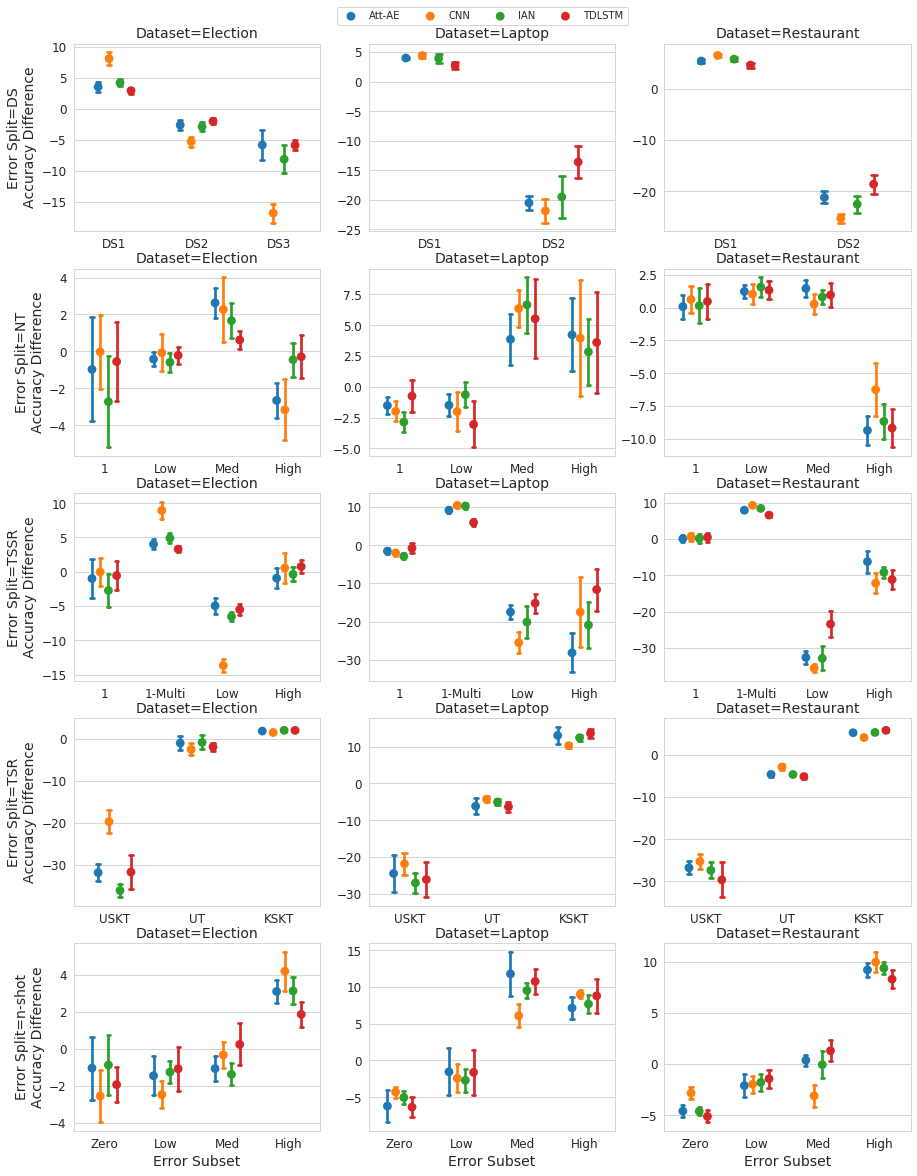
\includegraphics[scale=0.3]{images/augmentation/methods_performance/baseline/test_error_diff_subsets.png}
    \caption{The mean and standard deviation error bars for the difference between the overall accuracy and the accuracy from each error subset within all of the error splits on the test split across all datasets.}
    \label{fig:aug_baseline_test_error_diff_subset}
\end{figure}

Using the test (validation) results from the subsets shown in figure \ref{fig:aug_baseline_test_error_subset} (figure \ref{fig:aug_baseline_validation_error_subset}) it is possible to explore the differences between the text classification model and the TDSA models. These differences can be better seen through the heatmaps in figures \ref{fig:aug_baseline_dataset_error_subset_heatmap} and \ref{fig:aug_baseline_combined_dataset_error_subset_heatmap}, where the former is not corrected for multiple significance tests where as the later is using Bonferroni and is aggregated across datasets. Note that for figure \ref{fig:aug_baseline_dataset_error_subset_heatmap} the $DS_3$ subset results should be ignored for the Laptop and Restaurant datasets as they were never calculated as the sample size for the $DS_3$ subset is too small. Also the $DS_3$ subset is removed from figure \ref{fig:aug_baseline_combined_dataset_error_subset_heatmap} as only the Election dataset contains enough samples to create confidence scores. From all of these figures it is clear to see that the subsets that the TDSA models outperform the text classification model in are $DS_2$, $DS_3$, \textit{low-TSSR}, \textit{TSR KSKT}, \textit{n-shot Med}, and \textit{NT Low}. There are other subsets where the difference is significant as shown in the heatmaps but the majority of these significant differences only occur because of the Election dataset as can be seen if you compare figures \ref{fig:aug_baseline_dataset_error_subset_heatmap} and \ref{fig:aug_baseline_combined_dataset_error_subset_heatmap}. Furthermore the outliers in these differences are the \textit{n-shot Med}, and \textit{NT Low} subsets of which the reason why it is believed these are outliers was described in the previous paragraphs. The $DS_2$, $DS_3$, and the \textit{low-TSSR} are expected to perform better for the TDSA models as they contain multiple unique sentiments within a sentence, for which a text classification model can only predict one of those sentiments for the sentence thus limiting the models capability to perform well on these subsets. This therefore shows that the TDSA models must be learning some target sentiment relationship model or else they would not be more competitive than the text classifier. The \textit{TSR KSKT} shows that when the TDSA models have seen a target enough times in a known sentiment context then they can perform a lot better than the text classification model and there respective overall accuracy. However it is the other subsets within \textit{TSR} that are of more interest showing the deficiencies of the TDSA models. The worse subset within \textit{TSR} is the \textit{USKT} of which this is the only subset where the text classification model in general perform significantly better (see figure \ref{fig:aug_baseline_combined_dataset_error_subset_heatmap}). TDSA models are most likely biasing the target representation towards a subset of sentiment classes for those targets and hence why the text classification models perform better on those targets. The \textit{UT} (\textit{n-shot zero} is the same subset) subset is an interesting result as it is dataset dependent as shown best in \ref{fig:aug_baseline_dataset_error_subset_heatmap}, in the Election dataset the TDSA models are better but in all other datasets the text classification model is better. This could be due to the size of the datasets as the Election dataset is much larger than the rest and therefore could allow the TDSA models to create better general target representations, thus allowing the models to leverage similarities with known targets. From the dataset heatmap figure \ref{fig:aug_baseline_dataset_error_subset_heatmap} it can be easily seen that on the Election dataset almost all subset are statistically significant compared to the Laptop and Restaurant dataset. This is most likely due to the Election dataset containing more targets per text (as can be seen in table \ref{table:augmentation_combined_dataset_statistics} \footnote{Dataset statistics for the splits (rather than the whole dataset) used in this section can be seen in table \ref{table:augmentation_splits_dataset_statistics}.}) and therefore far fewer texts within $DS_1$ which is the subset the text classification model is most suited to. Even though the text classifier does not perform  statistically significantly better than all the TDSA models on the Laptop and Restaurant datasets for $DS_1$ they are never worse. Furthermore as the Laptop and Restaurant datasets are mainly made up of $DS_1$ samples (see figure \ref{fig:aug_error_analysis_ds}) this is most likely the reason why the TDSA models are not statistically significantly better than the text classification models on these datasets.

\afterpage{%
    %\clearpage% Flush earlier floats (otherwise order might not be correct)
    \thispagestyle{document}
    \begin{landscape}% Landscape page
            \centering
            \begin{longtable}{|c|c|c|c|c|c|c|c|}
\hline
Name &  No. Sents(t) &  No. Targs (Uniq) &  ATS(t) & POS (\%) & NEU (\%) & NEG (\%) \\
\hline
Laptop &              1872 &         2950 (1181) &    1.58 &  1328 (45.02) &   628 (21.29) &   994 (33.69) \\
\hline
Restaurant &              2578 &         4722 (1528) &    1.83 &  2892 (61.25) &   829 (17.56) &   1001 (21.2) \\
\hline
Election &              4045 &        11899 (2179) &    2.94 &  1744 (14.66) &  4572 (38.42) &  5583 (46.92) \\
\hline
\multicolumn{7}{|p{0.9\linewidth}|}{No. Sents(t)=number of sentences that contain a target, No. Targs (Uniq)=Number of (unique) targets (all targets are lower cased), ATS(t)=Average Target per Sentence where the sentences must contain a target, LABEL (\%)=Number of LABEL samples (percentage of LABEL samples).} \\
\hline
\caption{Dataset statistics for each datasets where each dataset represent the combination of all the dataset's splits e.g. train, validation, and test.}
\label{table:augmentation_combined_dataset_statistics}
\end{longtable}
    \end{landscape}
    \clearpage% Flush page
}

\begin{figure}[ht!]
    \centering
    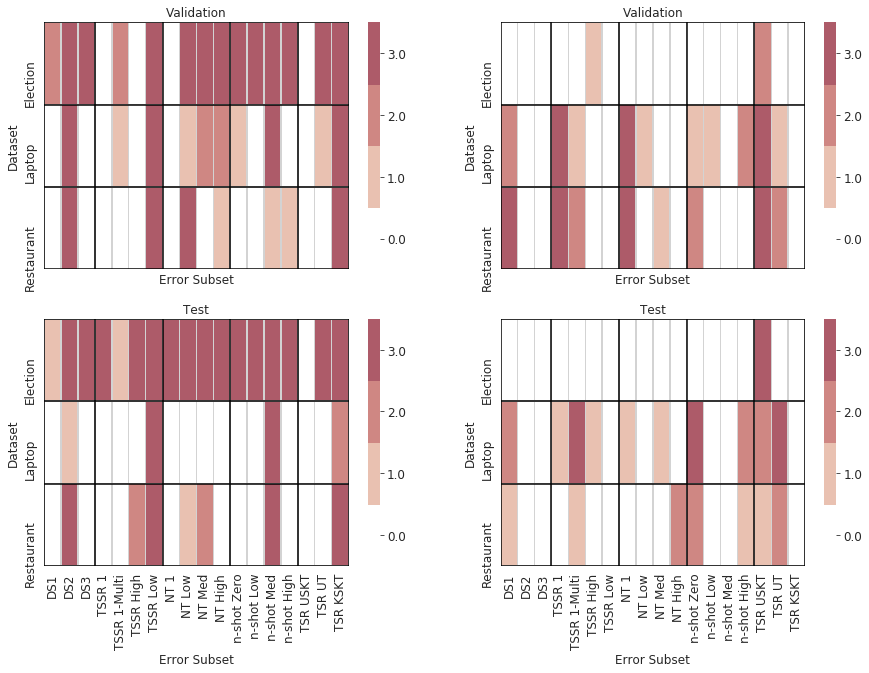
\includegraphics[scale=0.4]{images/augmentation/methods_performance/baseline/baseline_dataset_error_subset_heatmap.png}
    \caption{Plots in the first column represent the number of TDSA models that are statistically significantly better than the text classification model. Plots in the second column show the opposite, the number of TDSA models where the text classification is statistically significantly better. All plots have a confidence level of 95\% ($p \leq 0.05$).}
    \label{fig:aug_baseline_dataset_error_subset_heatmap}
\end{figure}

\begin{figure}[ht!]
    \centering
    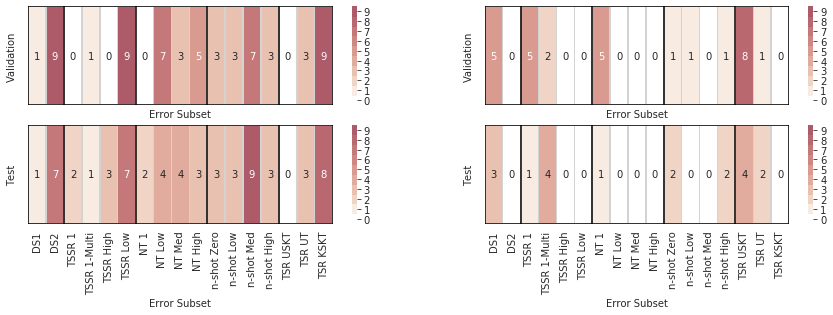
\includegraphics[scale=0.4]{images/augmentation/methods_performance/baseline/baseline_combined_dataset_error_subset_heatmap.png}
    \caption{Plots in the first column represent the number of TDSA models that are statistically significantly better than the text classification model across all datasets. Plots in the second column show the opposite, the number of TDSA models where the text classification is statistically significantly better. All plots have a confidence level of 95\% ($p \leq 0.05$) and have been corrected using Bonferroni.}
    \label{fig:aug_baseline_combined_dataset_error_subset_heatmap}
\end{figure}

% How does all of this relate back to the previous work this needs to be moved up to above the NT stuff.
From the results in this subsection the findings can relate back to some of the original work on these splits confirming the same findings. The findings of the \textit{TSSR 1-Multi} performing better than \textit{TSSR 1} is the same finding as \citet{nguyen-shirai-2015-phrasernn} as both of these subsets are the equivalent to \textit{ST2} and \textit{ST1}. When the number of unique sentiments increase in a text which can be measured through the \textit{DS} \textit{TSSR} split reduces the performance of methods is the same finding as \citet{xue-li-2018-aspect} comparing the normal test to the \textit{hard} test and that of \citet{nguyen-shirai-2015-phrasernn} comparing \textit{ST1} or \textit{ST2} with \textit{ST3}.  

The \textit{n-shot} findings do not confirm the findings of the original work by \citet{yang2018multi} where they found that in general models performance do not correlate with the number of times the target/aspect appeared in the training data. However our findings show that they do correlate where the more the target appears in the training data the better the performance in general. The reason for the difference could come from the task itself, as \citet{yang2018multi} was not solving the task of TDSA but rather the task of Multi-Entity Aspect Based Sentiment Analysis (ME-ABSA), where TDSA would be equivalent if when predicting the sentiment of the target the latent aspect was also given. This difference in task could make a large difference as knowing a target's latent aspect could greatly improve a models performance on unknown targets. The reason why the latent aspect would make such a large difference is because the dataset would contain a few aspects which occur frequently therefore allowing the model to create a good representation for the aspects. Furthermore given these aspects the likelihood is that there could be many unknown aspect target pairs but due to the model potentially having a good representation of the aspect the performance on these \textit{zero-shot} pairs could be quite high. Thus a reason for \citet{yang2018multi} finding no correlation between performance and number of times the target/aspect appeared in the training data could be due to the aspects.

%
% The above three paramgraphs need to be merged with the one below. as need to add a paragraph on DS
%
% The \textit{NT} split by \citet{zhang-etal-2019-aspect} which was found to be unstable in that original work and similar in this thesis, was to some extent explained empirically why it was for the first time in this thesis. The reason in \citet{zhang-etal-2019-aspect} work to overcome the stability was to better model inter target dependencies (target interaction). However considering the empirical evidence put forward here as shown in figures \ref{fig:aug_baseline_ds_nt_test_scores} and \ref{fig:aug_baseline_tssr_nt_test_scores}, the belief is that the \textit{NT} split itself does not measure target interaction and a dataset that does so would be a more suitable suggestion.

As found earlier in figure \ref{fig:aug_baseline_test_error_subset} (validation data figure \ref{fig:aug_baseline_validation_error_subset}) the \textit{NT} split does not show any consistent trend in one of the original works \citep{zhang-etal-2019-aspect} also found, of which the expected trend was as the number of targets increase the lower the performance. A potential reason for this could be that there are other factors that influence the \textit{NT} split. The factors that will be explored here are the target sentiment relationship factors which can be measured to some extent using the \textit{DS} and \textit{TSSR} splits. To explore this all the datasets will be first subsetted by one of the \textit{DS} or \textit{TSSR} subsets and then further subsetted by one of the \textit{NT} subsets, the models performance will be measured on each one of these compounded subsets. Figure \ref{fig:aug_baseline_ds_nt_test_scores} (\ref{fig:aug_baseline_ds_nt_validation_scores}) and \ref{fig:aug_baseline_tssr_nt_test_scores} (\ref{fig:aug_baseline_tssr_nt_validation_scores}) show the performance on these compounded subsets for the test (validation) data where the former subsets the data first by a \textit{DS} subset and the later by a \textit{TSSR} subset. Note that in the figures some of the \textit{NT} subsets do not exist on the x-axis this is because after the subset compounding no data exists for those subsets. These figures show that in general for the $DS_1$ and \textit{TSSR 1-Multi} rows the longer the sentence (larger \textit{NT}) the better the performance of the models, of which for $DS_1$ row this can be better seen in the validation data (figure \ref{fig:aug_baseline_ds_nt_validation_scores}) than the test. This is most likely the case because of the models exploiting the fact that there are more targets expressing the same sentiment. This exploitation of targets expressing the same sentiment can also be seen in the $DS_2$ rows (better seen in the validation data) where the more targets the better the score. Within the \textit{Low} and \textit{High TSSR} subsets the trend is less clear. The expectation within these subsets would be, the \textit{Low (High) TSSR} subset that when there are more (less) targets (higher \textit{NT}) the worse the results. This expectation is under the assumption that the more targets in \textit{High (Low)} the more (less) targets that have the same sentiment and thus exploiting the most frequent sentiment would gain a higher (lower) accuracy score. However this expectation is not always true and can be in-consistent between splits for example the \textit{High TSSR} Laptop results have different trends between test and validation splits. Furthermore this assumption of more targets within the \textit{TSSR Low} and \textit{High} subsets does not necessarily mean more targets of the most frequent sentiment class due to the way \textit{TSSR} subsets are created (equation \ref{eq:aug_tssr}), hence a potential reason why there is no consistent correlations in those subsets. Thus this analysis shows to some extent why the \textit{NT} split has no trend as the target sentiment relationship factors are more influential than the number of targets on the performance of the models. This therefore solves to some extent why \citet{zhang-etal-2019-aspect}\footnote{See figure 4 in the paper.} and also could not find a steady trend for the \textit{NT} split.
%The $DS_2$, $DS_3$, \textit{High TSSR}, and \textit{Low TSSR} rows are less clear most likely due to the $DS_2$ and $DS_3$ containing data that can be in both \textit{Low} and \textit{High} \textit{TSSR} subsets. Thus as stated earlier the model could be overfitting to one sentiment in each sentence and hence why there are trends in the \textit{Low (High) TSSR} subset that when there are more (less) targets (higher \textit{NT}) the worse the results. This analysis shows that there are trends in the \textit{NT} subsets when sentiment relation factors have been taken into account as shown by subsetting the data first by one of the \textit{TSSR} or \textit{DS} subsets. Thus this analysis shows to some extent why the \textit{NT} split has no trend as the target sentiment relationship factors are more influential than the number of targets on the performance of the models. This therefore solves to some extent why \citet{zhang-etal-2019-aspect}\footnote{See figure 4 in the paper.} also could not find a steady trend for the \textit{NT} split. 

%This analysis however brings up the question of how to measure target interaction explicitly as the \textit{NT} split clearly cannot do this. Thus a dataset that has target interaction annotated would be of use to the community to better understand these models. However careful consideration will have to be taken when creating such a dataset so that other factors are not being measured at the same time. One could design such a dataset so that the only way a target can be predicted is through target to target interaction, and not possible via target sentiment relationship or most frequent sentiment class within the sentence. Thus it can be concluded that the \textit{NT} split is not fit for any purpose therefore will not be used after this subsection.

\begin{figure}[h!]
    \centering
    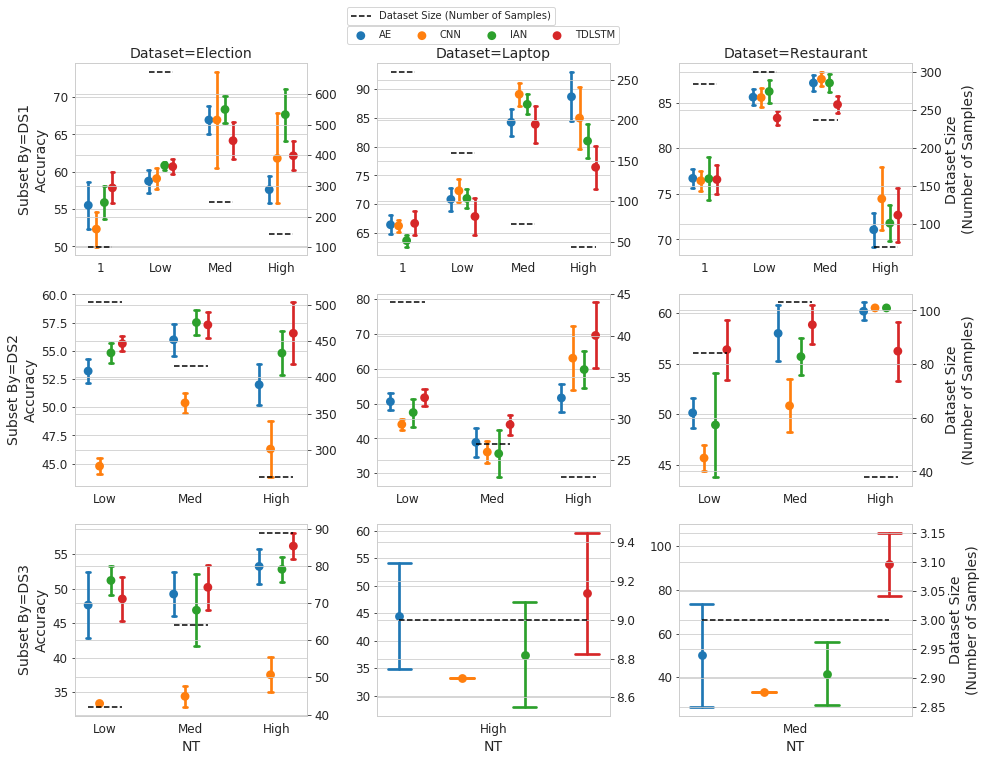
\includegraphics[scale=0.35]{images/augmentation/methods_performance/baseline/baseline_ds_nt_test_scores.png}
    \caption{Each plot shows the performance (y-axis accuracy) of the given models and sample size of the data evaluated on (y-axis dataset size) on the different test datasets (columns) after being subsetted by the relevant \textit{DS} subset (rows) and then NT subset (x-axis).}
    \label{fig:aug_baseline_ds_nt_test_scores}
\end{figure}
\begin{figure}[h!]
    \centering
    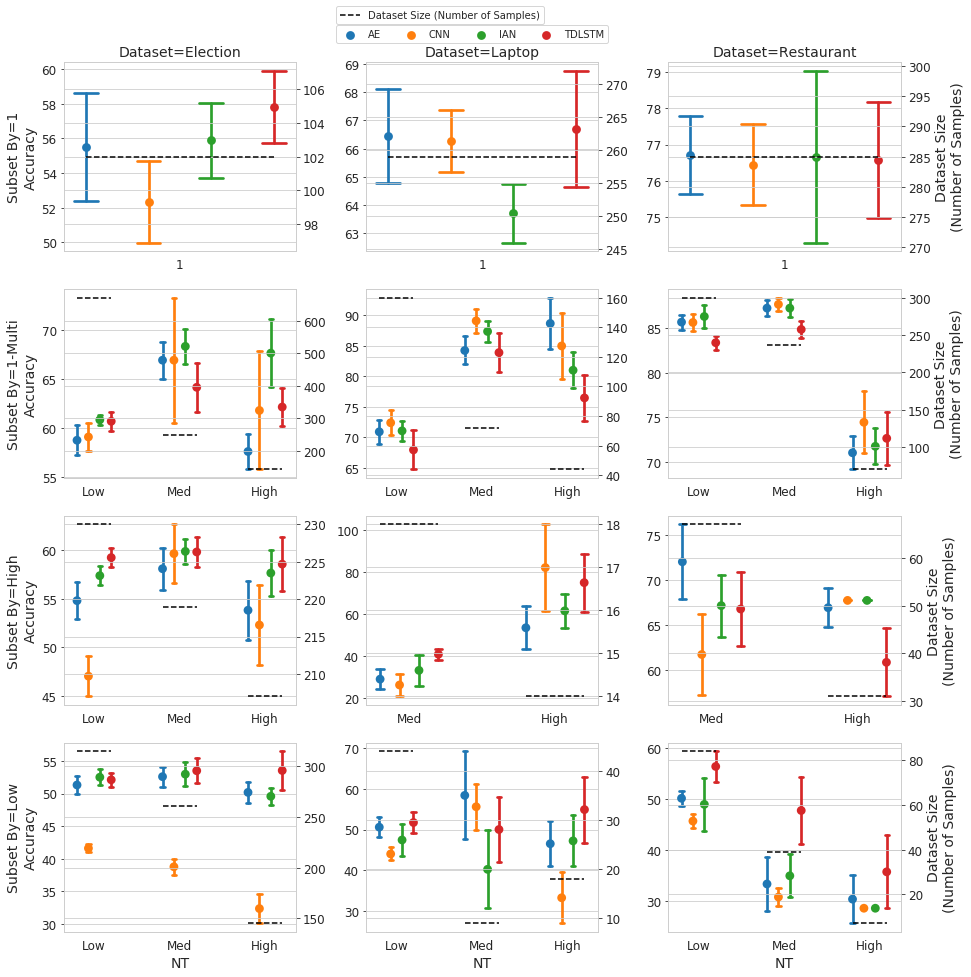
\includegraphics[scale=0.35]{images/augmentation/methods_performance/baseline/baseline_tssr_nt_test_scores.png}
    \caption{Each plot shows the performance (y-axis accuracy) of the given models and sample size of the data evaluated on (y-axis dataset size) on the different test datasets (columns) after being subsetted by the relevant \textit{TSSR} subset (rows) and then NT subset (x-axis).}
    \label{fig:aug_baseline_tssr_nt_test_scores}
\end{figure}

The $DS_i$ split was  was stated to get more difficult as $i$ increased and this has been shown in this work and in the original \citep{wang-etal-2017-tdparse}. However as mentioned in the last section \ref{section:aug_error_analysis_previous_work}, in the original work it was also shown for some methods and metrics that the models perform best on the $DS_3$ subset. In this work that phenomena did not occur when using the accuracy metric, of which \citet{wang-etal-2017-tdparse} did not use this metric. Therefore to test if the \textit{DS} split results do change based because of the metric in figure \ref{fig:aug_baseline_sentiment_f1_ds_all} are the \textit{DS} results on across all datasets using the macro F1 metric which was one of the metrics used by \citet{wang-etal-2017-tdparse}. As can be seen from the results the only dataset where $i$ in $DS_i$ does not negatively correlate with the macro F1 results is the Election test dataset. The Election test datasets was also the only dataset \citet{wang-etal-2017-tdparse} used when measuring models performance on the \textit{DS} split\footnote{Results can be found in table 4 of \citet{wang-etal-2017-tdparse}.}. The other results follow the trend shown in this section when using the accuracy metric. 

\begin{figure}[h!]
    \centering
    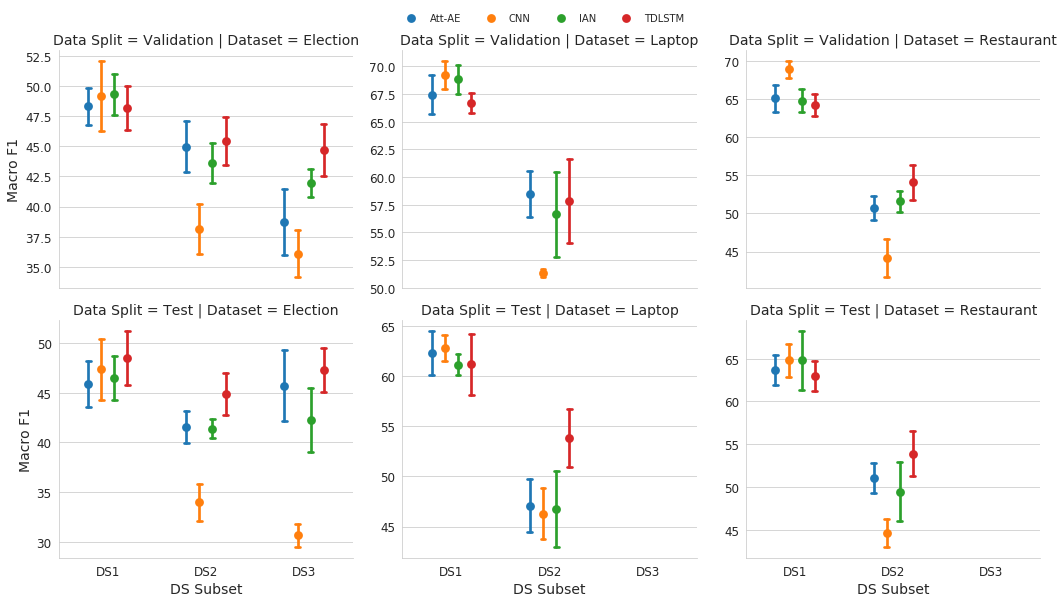
\includegraphics[scale=0.3]{images/augmentation/methods_performance/baseline/sentiment_f1_ds_all.png}
    \caption{Macro F1 score where the data has subsetted by the \textit{DS} split.}
    \label{fig:aug_baseline_sentiment_f1_ds_all}
\end{figure}

To investigate why the Election test dataset does have a different trend when using a different metric the approach taken was to explore the individual F1 scores for each sentiment label on the Election dataset. This approach was taken as the main difference between accuracy and macro F1 is the macro F1 is not biased by the un-balanced label distribution that is within the dataset, of which all datasets used are very un-balanced see table \ref{table:augmentation_combined_dataset_statistics}. Figure \ref{fig:aug_baseline_sentiment_f1_ds_election} shows the results of each sentiment labels F1 score and as expected the most frequent sentiment (negative) has the highest scores no matter the subset. These results highlight why the macro F1 score does not have the same negative correlation as the accuracy metric does for the \textit{DS} split. As the results show the positive and the neutral sentiments do not follow the negative correlation that the negative sentiment does. Thus as the scores of each sentiment are weighted the same in the macro F1 metric this therefore causes the macro F1 score for the $DS_3$ subset to be higher than the $DS_2$ subset in the test split. The potential reason for this unusual correlation could be due to the model overfitting to the most frequent sentiment class (negative) and hence why if the model predict negative for all samples in a $DS_3$ sentence then it would get some samples correct but it would get at least 2 samples wrong.

\begin{figure}[h!]
    \centering
    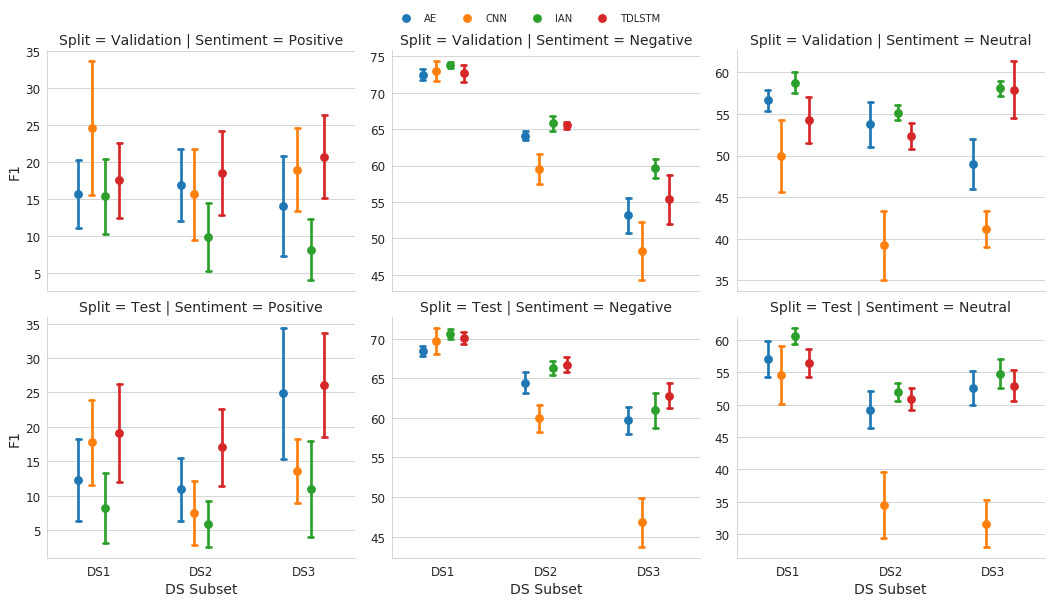
\includegraphics[scale=0.3]{images/augmentation/methods_performance/baseline/sentiment_f1_ds_election.png}
    \caption{The Election test and validation split F1 scores for each sentiment label, where the data has been further broken down through \textit{DS} subsets.}
    \label{fig:aug_baseline_sentiment_f1_ds_election}
\end{figure}

To further investigate whether the most frequent sentiment class always has this negative correlation the results for the Restaurant and Laptop datasets are shown in figures \ref{fig:aug_baseline_sentiment_f1_ds_restaurant} and \ref{fig:aug_baseline_sentiment_f1_ds_laptop} respectively. From these two plots we can see that the most frequent sentiment class (positive for both datasets) has the largest drop in F1 score from $DS_1$ to $DS_2$. This large drop in F1 score gives some extra merit to the idea that the models are overfitting to the most frequent sentiment class. Due to this overfitting the model is most likely predicting the most frequent sentiment class more often than it should where as in the cases for the least frequent sentiment classes it could be only predicting these when it is confident. These reasons are not empirically proven but the results have shown further insight into the \textit{DS} split. Lastly these results show more that the results from the original paper \citet{wang-etal-2017-tdparse} do not generalise across datasets and that the general result is that the metrics normally correlate negatively with the \textit{DS} subsets. 

\begin{figure}[h!]
    \centering
    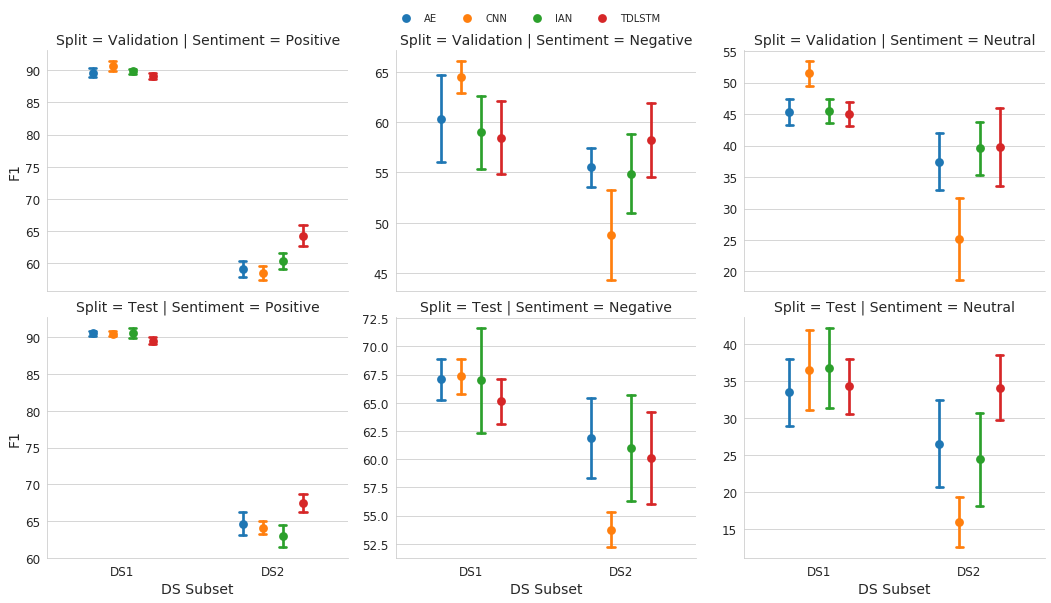
\includegraphics[scale=0.3]{images/augmentation/methods_performance/baseline/sentiment_f1_ds_restaurant.png}
    \caption{The Restaurant test and validation split F1 scores for each sentiment label, where the data has been further broken down through \textit{DS} subsets.}
    \label{fig:aug_baseline_sentiment_f1_ds_restaurant}
\end{figure}
\begin{figure}[h!]
    \centering
    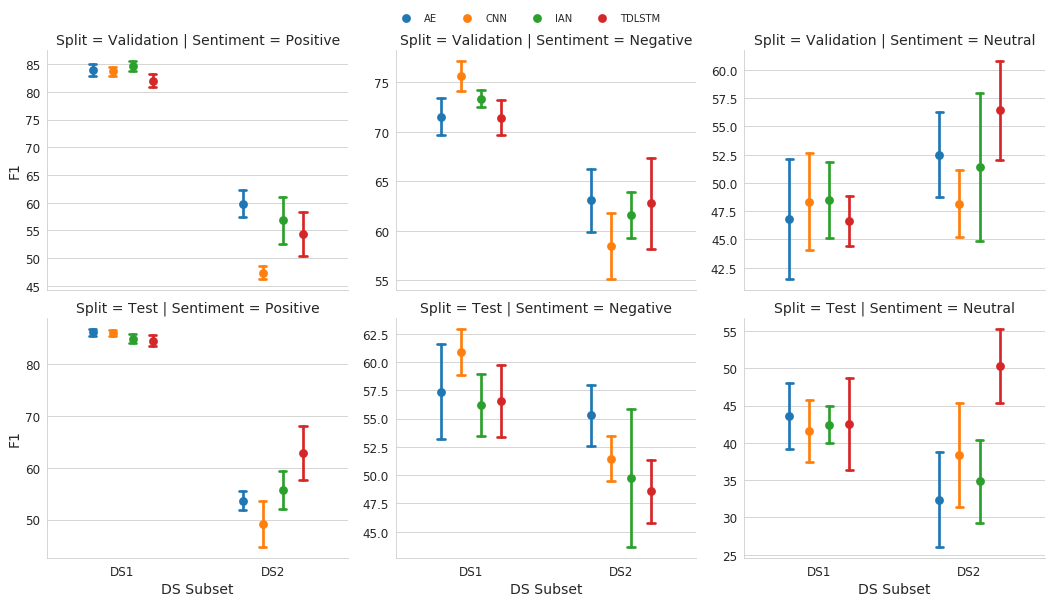
\includegraphics[scale=0.3]{images/augmentation/methods_performance/baseline/sentiment_f1_ds_laptop.png}
    \caption{The Laptop test and validation split F1 scores for each sentiment label, where the data has been further broken down through \textit{DS} subsets.}
    \label{fig:aug_baseline_sentiment_f1_ds_laptop}
\end{figure}

Both the \textit{DS} and \textit{TSSR} error splits explore the concepts of target sentiment relationships and overfitting to the most common sentiment within a text. However neither of these can create error subsets that will explicitly inform you if the model can detect sentiment for all the targets in the text and thus performing the target sentiment relationship task perfectly. Both the \textit{DS} and \textit{TSSR} splits do attempt to show this but both are subject to the model finding the most frequent or easiest to find sentiment for some/all of the targets in the subsets. Thus the creation of the Strict Text ACcuracy (\textit{STAC}) metric. This metric works on the sentence/text level compared to the accuracy and macro F1 metrics that are based at the target level. \textit{STAC} treats each sentence as a sample and each sentence can only be correct if all targets within that sentence have been classified correctly, it is then averaged by the number of sentences. The \textit{TAC} equation \ref{eq:aug_tac} that is used within the \textit{STAC} equation \ref{eq:aug_stac} finds the average number of targets that are correct within a sentence. The notation to describe \textit{STAC} and \textit{TAC} in equations \ref{eq:aug_stac} and \ref{eq:aug_tac} is the same as that in equation to describe the \textit{TSSR} split in equation \ref{eq:aug_tssr}. $T_j$ within \textit{STAC} represents all of the targets within sentence $j$ from all sentences $X$ that is within the dataset, and $t_{ji}$ represents target $i$ true sentiment within sentence $T_j$ where $\hat{t_{ji}}$ is the predicted sentiment.

\begin{equation}
    \text{Text ACcuracy (TAC)}(T_j) = \frac{\sum_{i=1}^{|T_j|} [t_{ji}=\hat{t_{ji}}]}{|T_j|}
    \label{eq:aug_tac}
\end{equation}
\begin{equation}
    \text{Strict Text ACcuracy (STAC)} = \frac{\sum_{j=1}^{|X|} \begin{cases}
    1,& \text{if } \text{TAC}(T_j) = 1\\
    0,              & \text{otherwise}
\end{cases}}{|X|}
\label{eq:aug_stac}
\end{equation}

The \textit{STAC} metric is more useful when applied to subsets of a dataset, thus two specific versions of the \textit{STAC} metric are created:
\begin{enumerate}
    \item \textit{STAC 1} - The \textit{STAC} metric applied to only the data in the $DS_1$ subset.
    \item \textit{STAC Multi} - The \textit{STAC} metric applied to only the data in the $DS_2$ and $DS_3$ subsets.
\end{enumerate}
From now on when the performance of models on \textit{STAC} assumes the \textit{STAC} metric has been applied to the whole dataset. The \textit{STAC Multi} gives in one metric how well overall a TDSA model is at target sentiment relation extraction removing all factors of overfitting to a sentiment class, or predicting the most frequent sentiment of which this is possible in \textit{STAC 1}. \textit{STAC Multi} can also be seen as a coarse grained and much stricter version of the \textit{DS} split, as both measure target sentiment relationship modelling. However due to \textit{STAC Multi} being such a strict and thus difficult metric the \textit{DS} subsets can be useful to measure target sentiment relationship modelling at a more fine grained scale. For example if a model does not perform significantly better nor worse than another on \textit{STAC Multi} but does perform better on $DS_2$ and $DS_3$ subsets, then the likelihood is that the model is performing target sentiment relationship modelling better. The difference between \textit{STAC 1} and \textit{STAC Multi} can show to some degree how much the model is exploiting the fact the sentence only contains one sentiment. The performance of all models across all metrics including accuracy and macro F1 can be seen in \ref{fig:baseline_stac_scores.png}, the \textit{STAC} metric is shown for completeness. As can be seen from the figure the \textit{STAC Multi} is by far the most difficult metric and scores much lower than any of the accuracy metrics on any of the subsets shown in figure \ref{fig:aug_baseline_test_error_subset} (validation split figure \ref{fig:aug_baseline_validation_error_subset}). However the \textit{STAC 1} results can be the easiest metric as shown by the Restaurant dataset. The difference between \textit{STAC 1} and \textit{STAC Multi} for the TDSA models is rather large and more so for the Restaurant and Laptop datasets which could be due to the fact there are proportionally and overall more $DS_2$ and $DS_3$ sentences in Election than the Restaurant and Laptop datasets as shown by table \ref{tab:aug_STAC_samples_stats}. Furthermore as should be the case the text classification model (\textit{CNN}) scores $0$ in all of the \textit{STAC Multi} thus showing again the point of the metric and the relevancy to TDSA. These scores highlight that TDSA models have much to improve upon with regards to target sentiment relation modelling as shown by the \textit{STAC Multi} metric without resorting to simpler majority sentiment classification of the sentence as shown by \textit{STAC 1}, and the other error subsets ($DS_1$, \textit{TSSR 1}, and \textit{TSSR 1-Multi}). Furthermore from the results it is interesting to see that \textit{TDLSTM} model generally performs well on the \textit{STAC Multi} metric compared to the other models across all datasets, of which this could be due to the model encoding position of the target within it's architecture. 

\begin{figure}[ht!]
    \centering
    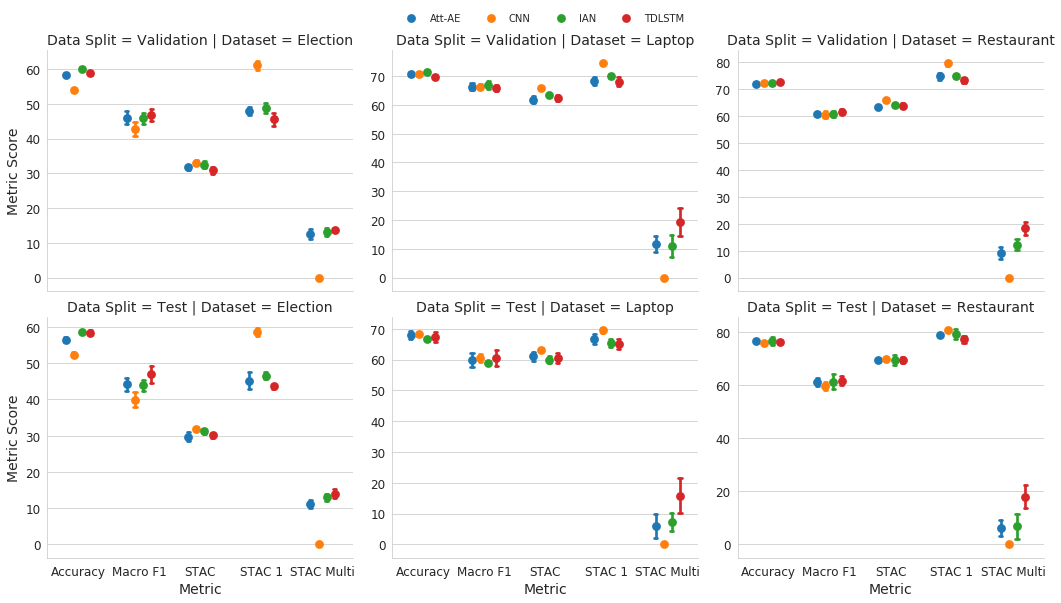
\includegraphics[scale=0.32]{images/augmentation/methods_performance/baseline/baseline_stac_scores.png}
    \caption{Performance across all metrics for all models across all datasets and splits.}
    \label{fig:baseline_stac_scores.png}
\end{figure}

\begin{table}[ht!]
    \centering
    \begin{tabular}{|c|c|c|c|c|}
\hline
& & \multicolumn{2}{c|}{Subset} & \\
\hline
Split & Dataset &  $DS_1$ &  $DS_2$ and $DS_3$ &  Total \\ 
\hline
\multirow{3}{*}{Train} & Election   &    1227 &  1092 & 2319 \\
& Laptop     &    933 &  118 &  1051 \\
& Restaurant &    1162 &  216 & 1378 \\
\hline
\multirow{3}{*}{Validation} & Election   &    467 &  396 & 863 \\
& Laptop     &    364 &  47 &  411 \\
& Restaurant &    497 &  103 & 600 \\
\hline
\multirow{3}{*}{Test} & Election   &    469 &  394 & 863 \\
& Laptop     &    373 &  38 &  411 \\
& Restaurant &    520 &  80 & 600 \\
\hline
\end{tabular}
    \caption{Number of sentences in each split for all datasets.}
    \label{tab:aug_STAC_samples_stats}
\end{table}


Through these subsets and new metrics (\textit{STAC}) we can see the differences between the TDSA and text classifier and where the TDSA models do outperform the text classifier by a large margin. The flip side to distinguishing the performance of TDSA and text classifier models is by creating `challenge datasets' that examine the performance of a model in specific circumstances. This approach was taken by \citet{jiang-etal-2019-challenge} where they created a new version of the Restaurant dataset called Multi-Aspect Multi-Sentiment (MAMS). The MAMS dataset as the name suggests only contain texts that have at least two targets with at least two different sentiments, thus removing all texts that only have one sentiment. This new dataset was created to avoid samples being easily classified by a text level classifier. This dataset therefore fits into the $DS_2$ and $DS_3$ only subsets from the \textit{DS} split. They found a large difference in scores between the text classifier models and the TDSA ($\geq 10\%$), which is what was found in the error subset analysis earlier in this subsection on all datasets as shown in figures \ref{fig:aug_baseline_test_error_subset} and \ref{fig:aug_baseline_test_error_diff_subset}. However to overcome this problem they have had to create a new dataset which costs in either money and/or time, which is not the case in the error subset approach shown here. The approach of creating new datasets to examine properties of TDSA models is not scalable without large resources thus the error subset approach is a very feasible alternative and as shown affective. Furthermore using the new \textit{STAC-Multi} metric it is now possible to quantify TDSA model performances on samples that only TDSA models can correctly predict. This does not mean that these challenge datasets are not useful, for instance using this dataset can help answer the question of whether using more $DS_2$ and $DS_3$ samples will improve TDSA models performance on those subsets and how much would that affect the performance on the $DS_1$ subset.


To conclude this subsection, the baseline experiments have brought about many different findings, of which some have confirmed prior findings, where as others have not. Unlike previous work it has been shown that TDSA models on datasets that do not contain a lot of targets per text such as the Laptop and Restaurant datasets can be statistically no better than a text classifier, prior work has shown this in absolute performance but not statistically \citep{jiang-etal-2019-challenge}. From these baseline experiments we can conclude that all the error splits have been successfully tested across a range of models and datasets. From analysing the error split results the baseline TDSA models generally perform best on subsets of data that contain one unique sentiment ($DS_1$) and on targets that appear multiple times in different sentiment classes within the training data (\textit{KSKT}). This finding suggests that the baseline models are very brittle and cannot generalise to unknown targets (\textit{UT}), unknown sentiment relations (\textit{USKT}) or texts that contain multiple unique sentiments ($DS_2$ and $DS_3$). Due to these factors the models are unlikely to perform well in low resourced or cross domain settings. The subsection also introduced a novel TDSA metric \textit{STAC} and its two variants \textit{STAC-Multi} and \textit{STAC 1} of which when used together can show sentiment overfitting to the most frequent sentiment class in a text to some extent. Furthermore the \textit{STAC-Multi} shows how well the TDSA models can perform target sentiment relationship modelling perfectly, as well as how the \textit{DS} subsets are a fine grained and easier version of \textit{STAC Multi}.

The subsection has related back to the original work that created these error splits in doing so explained why the \textit{NT} split does not have a consistent trend. From exploring the different splits many of them have been dismissed due to the results not matching the hypothesis of what the split is suppose to measure. Thus the \textit{NT} split, due to having no consistent trend, cannot be used to measure target interaction. The \textit{TSSR} split cannot measure sentiment overfitting, and the \textit{n-shot} split is not as useful as the \textit{TSR}. Therefore the recommended splits to use are the \textit{DS} for measuring fine grained target sentiment relation modelling and \textit{TSR} to measure the models ability to generalise to unseen targets and sentiment relationships. Furthermore the \textit{STAC-Multi} metric is recommended to measure target sentiment relation modelling as well but is a much stricter and coarser measure compared to \textit{DS} results. The \textit{STAC 1} should also be used so that it can show to some degree with \textit{STAC-Multi} the extent of overfitting to the most frequent sentiment class in a sentence.

Lastly from exploring the results across these different splits future research directions have surfaced. Due to none of the splits being capable of explicitly measuring target interaction an annotated corpus incorporating this annotation would be of use. \citet{he-etal-2018-effective} has shown that using an un-supervised autoencoder objective to mimic encoding a latent aspect into the target representations improves general results as well as results on multi word targets, and visually has shown on selected targets to create better target representations. However it would be of interest to see if such a method can help target representations for unknown targets (\textit{UT}) as this would be similar to the Multi-Entity Aspect Based Sentiment Analysis (ME-ABSA) task, where \citet{yang2018multi} had found no difference between \textit{UT} and Known Sentiment Known Targets (\textit{KSKT}). Thus suggesting that encoding the latent aspect could greatly benefit the \textit{UT} samples.


%3. Even though TSSR was mainly created to measure sentiment overfitting, through differences in the High and Low subset scores, this overfitting measure is a somewhat more fine grained version from the STAC metric. In the STAC metric the gap between STAC Multi and STAC 1 is normally large and this can be due to overfitting, but is more likely due to the model getting just one prediction wrong, hence why the gap between High and Low is much smaller. Thus when the sample size is large enough in the High and Low TSSR subsets this is another good measure of overfitting to the most frequent sentiment class without the requirement of having to predict all targets correctly. 4. The DS subsets show on a discrete scale the extent to which the TDSA models can detect sentiment relations, where the better it is at the top end of the scale DS3 the more likely the model is performing sentiment relation extraction on each target. This can be seen as a more fine grained analysis on the STAC Multi metric where this metric is an extremely difficult version of the DS3 and DS2 subsets. Furthermore this can empirically be seen in the analysis, where the TDLSTM model performs best in the STAC Multi metric and also performs in the top 2 of the DS3 subset on the Election dataset in both splits compared to the ATT-AE which performs worse in the TDSA models in both DS3 and STAC Multi.5. The n-shot subset can measure to some extent the ability of a model to generalise to new targets. However the TSR subsets results shows this more explicitly due to the subsetting the data based on both the target occurrence and the occurrence of the target with a sentiment class in the training data. Due to this it can be seen that even if a target is known it can perform badly on that target if the sentiment associated to it has not be seen before in the training data. This finding can possibly explain why the n-shot subsets do not show a positive correlation between n and the metric score. Furthermore the TSR KSKT subset is always the best performing subset within the split unlike the high in the n-shot. Thus for exploring a models ability to generalise to unknown targets and unknown sentiment relations TSR is recommended compared to n-shot as both of these subsets can be compared to KSKT subset as the upper limit as KSKT can be seen as the data rich subset.

\section{Position Encoding}
\label{section:aug_position_encoding}
\subsection{Introduction}
This is the first model enhancement that will be explored in this chapter. As stated in the introduction section \ref{section:aug_method_performance_intro}, the two models that will be explored in this section are \textit{IAN} and \textit{Att-AE} due to the \textit{TDLSTM} already having position information somewhat encoded into its NN architecture. Within the prior work, position information has been encoded into different TDSA methods in broadly three different approaches; weighting, embedding, and via the construction of the NN architecture (construction). Position weighting is probably the simplest approach as it weights the vectors of tokens/words\footnote{Normally after they have been encoded via some sequence encoder e.g. LSTM.} based on some distance metric to the relevant target word(s). However there is no one standard distance metric in the literature but a lot of them are very similar; \citet{chen-etal-2017-recurrent} (equation 7 and section 3.3) based the weighting on how many tokens are between the context word and the nearest target word (token) and then normalised via sentence length\footnote{They further encoded the relative position of the word into the model.}. Other methods have created an arbitrary cut off so that context words that are too distant are ignored \citep{he-etal-2018-exploiting, zhao2019modeling}, \citet{zhang-etal-2019-aspect} uses the same weighting as \citet{chen-etal-2017-recurrent} but ignores the target words. \citet{he-etal-2018-exploiting} incorporated syntax into the weighting where the position to the target word(s) is defined by the distance through the dependency tree. Lastly \citet{li-etal-2018-transformation} used the same weighting as \citet{chen-etal-2017-recurrent} but normalises using an arbitrary constant rather than the sentence length ($n$).  In most cases across all of the experiments within the prior work on position weighting when the work has shown ablation studies position weighting has increased the performance of the models\footnote{The only work that has shown position weighting to harm performance is \citet{zhang-etal-2019-aspect} on the Twitter and Rest14 datasets in table 3.}. Position embeddings unlike the weighting mechanism encodes the position of a token/word via a learnt embedding space. Position embeddings are similar to the weighting mechanism in that they create position indexes that are relative to the target, where the indexes are created similar to the weighting mechanism. These position indexes for each word are calculated based on token distance from the closest target word. These position indexes, unlike the weighting method, are integers not floats as these integers are then used as an index to the random initialised (position) embedding. These position embeddings are then normally concatenated onto the word embeddings that represent the tokens in the sentence that the target occurs in \citep{gu-etal-2018-position, li-etal-2018-hierarchical, chen-qian-2019-transfer, sun-etal-2019-aspect, kumar2020aspect}. Unlike the position weighting literature all prior works that have used position embeddings calculate the position indexes based on relative distance to the nearest target token. Out of the five prior works, three use a position embedding dimension of 100, one uses 50, and another 30\footnote{Another prior work does not state the dimension of the position embeddings \citep{du-etal-2019-capsule}.}.  For clarification on position weighting and embeddings, table \ref{tab:aug_examples_position_indexes_weighting} shows an example text that has been tokenised where the target that is being predicted for is `Apple Mac', beneath each token is the weighting value and position index where the weighting value is calculated using equation \ref{eq:aug_chen_position}, which has come from \citet{chen-etal-2017-recurrent}. In equation \ref{eq:aug_chen_position}, $i$ represents the index of the token/word whose position is to be weighted, $\tau$ represents the index of the closest target token to $i$, and $n$ is the length of the text in tokens. 

\begin{equation}
    w_i = 1 - \frac{|\tau - i|}{n}
    \label{eq:aug_chen_position}
\end{equation}

\begin{table}[!h]
    \centering
    \begin{tabular}{|c|c|c|c|c|c|}
    \hline
         Tokens: & The & Apple & Mac & is & great  \\
    \hline
         Position indexes & 1 & 0 & 0 & 1 & 2 \\
    \hline
         Position weighting & 0.8 & 1 & 1 & 0.8 & 0.6 \\
    \hline
    \end{tabular}
    \caption{Example text which contains the target `Apple Mac', where the text has been tokenised and the associated position indexes and weightings are shown.}
    \label{tab:aug_examples_position_indexes_weighting}
\end{table}

Construction based approaches have used numerous different NN methods. \citet{tang-etal-2016-effective} (\textit{TDLSTM}) used RNNs where a forward RNN would process all tokens up to the last target token and a backward RNN for all tokens to the first target token. Other approaches have split the sentence up into left, right, and target contexts and aggregated the word embeddings using Neural Pooling methods \citep{vo2015target, zhang2016gated} or using a RNN based sequence encoder \citep{liu-zhang-2017-attention}. Another direction is to make use of a dependency parser to explicitly model the syntactic structure of the target's position, \citet{dong-etal-2014-adaptive} re-ordered the dependency tree to ensure the target word is the root and then used a Recursive NN (RecNN). \citet{sun-etal-2019-aspect, huang-carley-2019-syntax} both use the dependency tree without re-ordering it and apply a Graph NN (GNN) to encode words that are close to the target word through the dependency tree. \citet{nguyen-shirai-2015-phrasernn} used both a dependency and constituency parser to create a phrase dependency tree where the the tree is re-ordered such that the target word phrase is always at the root of the tree, they then used a RecNN to encode the tree data. Lastly one prior work has combined both position embeddings and a position based architecture \citep{sun-etal-2019-aspect}.

From this prior literature, the main reason for using position information is to create a more explicit bias in the model. The bias assumes that words that are closer to the target word(s) are more important and therefore should be given more weight, attention, or priority in the model. This bias is more or less explicit depending on the method used, in the case of weighting it is more explicit as words that are closer are always weighted higher than those further away. In comparison the embedding approach can be less biased as it allows the model to chose what words are closer and more important through the embedding. The construction method is hard to compare to the embedding and weighting approaches on bias as these approaches to some degree change their whole model so that position information is prioritised. In the case of \textit{TDLSTM} \citep{tang-etal-2016-effective} the bias of relatively close words are prioritised, compared to \citet{dong-etal-2014-adaptive} where they prioritise the syntactic distance between tokens and the targets words. 

In general, encoding position information is used to improve the performance on sentences that contain multiple targets as it should help match relevant words with their respective target \citep{li-etal-2018-hierarchical, he-etal-2018-exploiting}. This indicates that the point of position encoding is help improve target sentiment relation modelling. From these position encoding papers \citet{he-etal-2018-exploiting} is the only one to quantitatively evaluate the importance of position information further than just using overall metrics on the entire dataset. \citet{he-etal-2018-exploiting} have shown that using syntactic position weighting improves the performance for sentences that contain more than one target. The way this was evaluated was in effect using the \textit{NT} splits where they subsetted the data based on 1, 2, 3, and more than 3 targets per text. As has been shown in the last subsection \ref{section:aug_baseline} that the performance on the \textit{NT} split tends to be dominated by sentiment factors and does not directly measure target sentiment relationships. Even though \citet{he-etal-2018-exploiting} has performed a good quantitative evaluation, this cannot determine if the position information is actually improving target sentiment relation modelling. Therefore in this section position encoding will be evaluated across the two TDSA methods using the recommended error splits from the last subsection \textit{DS} and \textit{TSR} as well as using the TDSA specific metrics \textit{STAC Multi} and \textit{STAC 1}. In doing so, position encoding will be thoroughly evaluated for target sentiment relation modelling that it is claimed to do from the literature, as well as exploring any other positive or negative side affects. Furthermore the \textit{NT} subsets will also be included in the evaluation to demonstrate the point of why this split is not suitable for error analysis as it has been used in the prior work \citep{he-etal-2018-exploiting}. 

Given this prior literature the position encoding that will be used in this section is position weighting. This was chosen as it requires no extra parameters unlike the position embeddings and does not require fundamentally changing the NN architecture. The distance metric proposed by \citet{chen-etal-2017-recurrent} as shown in equation \ref{eq:aug_chen_position} will be used as it does not require any arbitrary cut off or normalising parameter to be tuned \citep{zhao2019modeling, li-etal-2018-transformation}, nor does it mask any words \citep{zhang-etal-2019-aspect}, and finally does not require a dependency parser \citep{he-etal-2018-exploiting}. Furthermore as this weighting method does not remove any words it allows the model to ignore the explicit bias of the position weighting in cases where the closest words are not always the most important e.g. in the case that the affecting opinion word(s) are a few syntactic hops away from the target. The position weighting will be applied to the context/sentence vectors after being encoded by the LSTM layer and before the attention is applied in both \textit{IAN} and \textit{Att-AE}.

\subsection{Experiments}

Figure \ref{fig:aug_overall_position_scores} shows the overall scores of the position encoded \textit{IAN} and \textit{Att-AE} models. These scores are somewhat meaningless without comparing them to their respective non-position encoded baseline models.

\begin{figure}[h!]
    \centering
    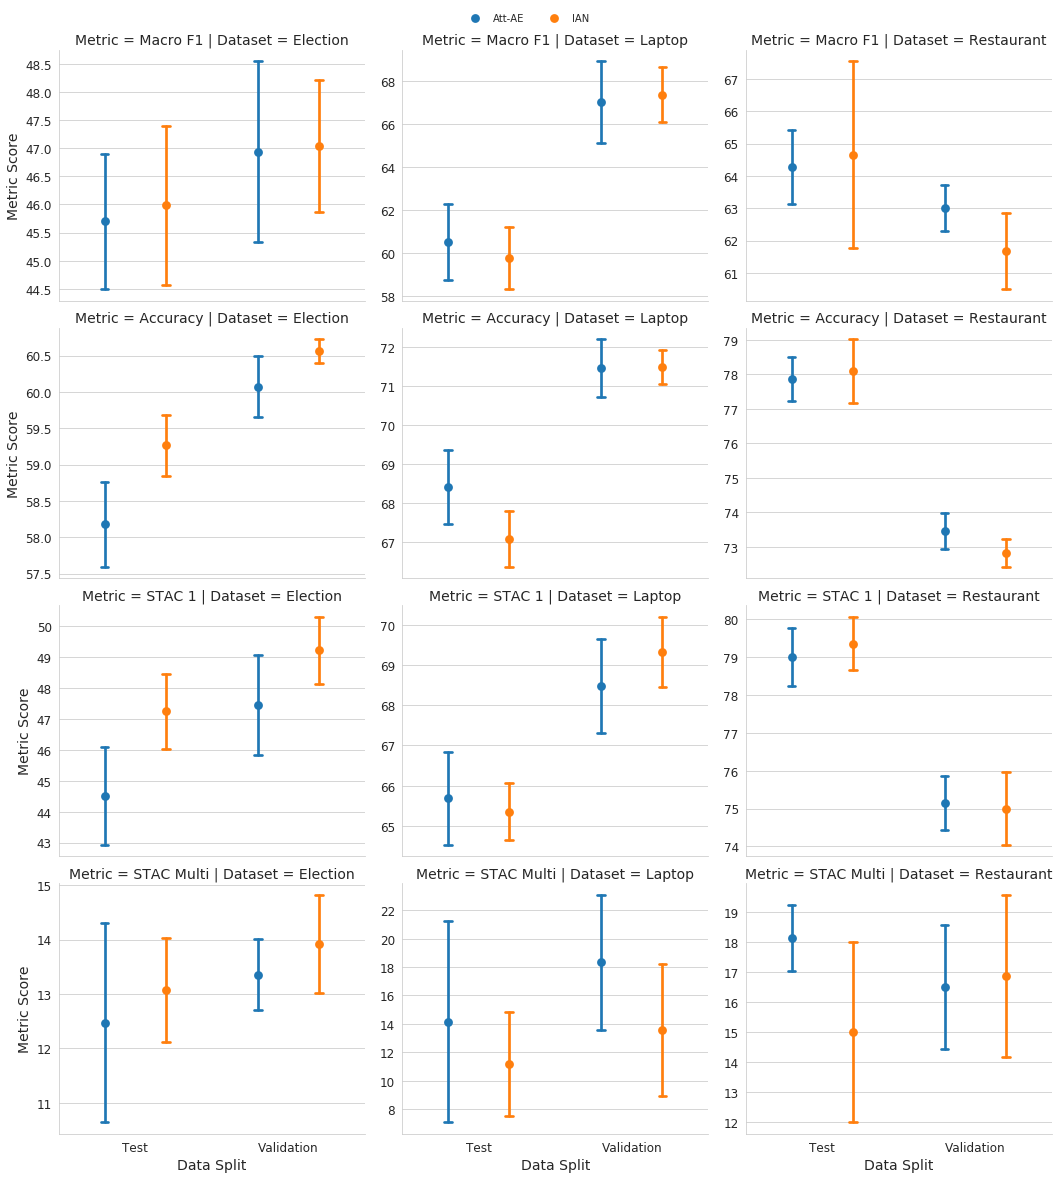
\includegraphics[scale=0.32]{images/augmentation/methods_performance/Position_Encoding/overall_position_scores.png}
    \caption{Columns represent different datasets, rows different metrics. Each plot represents the two position encoded models metric score on the test and validation splits.}
    \label{fig:aug_overall_position_scores}
\end{figure}

Figure \ref{fig:aug_position_baseline_overall_differences} shows the metric score difference between the position and the respective baseline models. As we can see from the results the overall trend is that, no matter the dataset or metric, position weighting on average improves the models performance. There are a few exceptions to this the \textit{STAC 1} results for both Election and Laptop datasets, and the \textit{accuracy} metric for the Laptop dataset. Furthermore there are several results where even though the mean is positive the standard deviations are so large that they go into the negative of the metric score difference. This shows that the trend might show an overall improvement in performance but the improvement is marginal.

%Finally the metric that appears to have the largest benefit from position weighting is the \textit{STAC-Multi} which does suggest that position weighting does improve the target sentiment relationship modelling, confirming the hypothesis from the literature about position weighting. Further this may explain the reason why \textit{TDLSTM} performed consistently better than the rest in the baseline results for the \textit{STAC-Multi} metric (see figure \ref{fig:baseline_stac_scores.png}) due to it having position information encoded into it NN architecture.

\begin{figure}[h!]
    \centering
    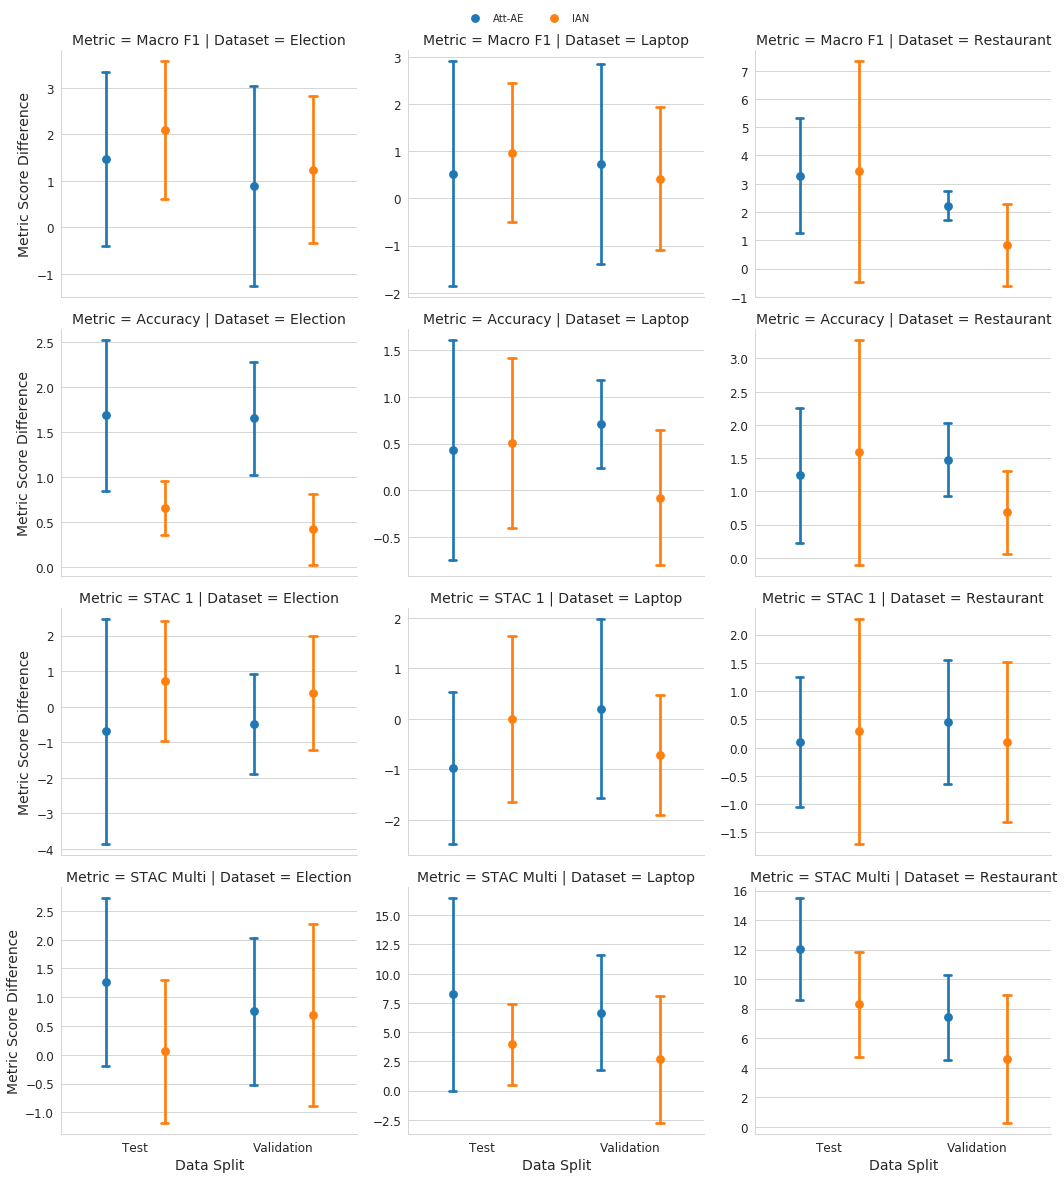
\includegraphics[scale=0.32]{images/augmentation/methods_performance/Position_Encoding/position_baseline_overall_differences.png}
    \caption{Columns represent different datasets, rows different metrics. Each plot represents the differences between the position and baseline models for the relevant metric score on the test and validation splits.}
    \label{fig:aug_position_baseline_overall_differences}
\end{figure}

To better visualise the differences figures \ref{fig:aug_position_overall_sig_models} and \ref{fig:aug_position_corrected_overall_sig_models} show the number of models that are significantly better than their baseline, where the former is not corrected for multiple significance tests where as the later is using Bonferroni and is aggregated across datasets. There were no models on any of the metrics or dataset splits where the baseline models were significantly better than the position models\footnote{The p-values for comparing the position to their baseline models can be found in table and the baseline to the position models in table}. From these heatmaps it can indeed be seen that the Restaurant dataset does benefit the most. 

As be seen from the heatmaps, the Laptop and the Restaurant datasets are the only datasets that consistently have position models that are significantly better on the \textit{STAC Multi} metric. Furthermore the Laptop dataset is the only dataset that does not find the position models to be consistently significantly better than the baselines on \textit{Accuracy}. This might not be a surprising finding considering that the Laptop dataset contains the least number of $DS_2$ and $DS_3$ samples relative to its size (see figure \ref{fig:aug_error_analysis_ds}). Thus as the findings suggest here that the position information improves the scores on the samples that have multiple unique sentiments within the sentences ($DS_2$ and $DS_3$), compared to a dataset that is made up of mainly sentences that only contain one unique sentiment. This reason is also related to another, of why position information does not perform significantly better on the \textit{STAC 1} metric. As the \textit{STAC 1} metric is only looking at the accuracy score for sentences that contain one unique sentiment and that the model predicts all samples in those sentences correctly. A model that overfits to the most frequent sentiment class will perform well on this metric. As the position information is biasing the model towards only looking at local context around the target it removes the bias for the model to look at the global context. This shows that biasing the model towards the local context through the position information removes some of the position overfitting that the baselines models exploited. It is clear to some degree that for at least the Laptop and Restaurant datasets that as the position models have improved on the \textit{STAC Multi} metric and not regressed on the \textit{STAC 1} metric, that the models are less prone to sentiment overfitting and do perform better at target sentiment relation modelling.

\begin{figure}[h!]
    \centering
    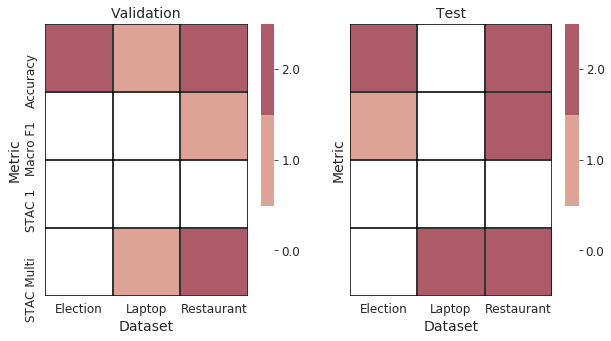
\includegraphics[scale=0.5]{images/augmentation/methods_performance/Position_Encoding/position_overall_sig_models.png}
    \caption{Heatmaps that represent the number of position models that are statistically significantly better than their baseline equivalents at the 95\% confidence level.}
    \label{fig:aug_position_overall_sig_models}
\end{figure}

\begin{figure}[h!]
    \centering
    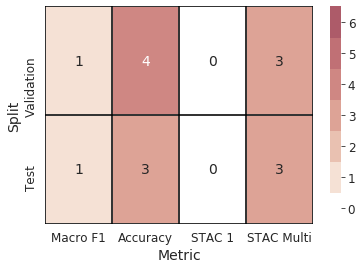
\includegraphics[scale=0.6]{images/augmentation/methods_performance/Position_Encoding/position_corrected_overall_sig_models.png}
    \caption{Heatmaps that represent the number of position models that are statistically significantly better than their baseline equivalents across all datasets at the 95\% confidence level. Where the multiple hypothesis tests have been corrected using Bonferroni.}
    \label{fig:aug_position_corrected_overall_sig_models}
\end{figure}

Furthermore from the heatmap results we can see that the Election dataset is the only one that the models do not perform significantly better than the baseline version on the \textit{STAC Multi} metric. However they do consistently perform better on the \textit{Accuracy} metric. This may suggest that the position information does improve the target sentiment relationship modelling but cannot be shown through the \textit{STAC Multi} metric as it requires all targets in the sentence to be correctly classified. The further reason why it is believed that it is improving the target sentiment relationship modelling rather than overfitting to the overall sentiment as the \textit{STAC 1} metric has not improved on the dataset. To investigate if the position models are improving the target sentiment relationship modelling on the Election dataset the results across all datasets for the \textit{DS}, \textit{TSR}, and \textit{NT} error splits are shown in figure \ref{fig:aug_position_split_difference_test_results} (\ref{fig:aug_position_split_difference_validation_results}) for the test (validation) split. The figure shows the difference between the position and respective baseline model\footnote{Figure \ref{fig:aug_position_split_overall_test_results} (\ref{fig:aug_position_split_overall_validation_results}) shows test (validation) results for the splits without subtracting from their respective baseline models.}. From this figure it is clear that that the position models improve the results for the $DS_2$ subset on the Restaurant and Laptop datasets. However for the Election dataset it would appear that the \textit{Att-AE} model is the one that benefits most from the position encoding (better seen in the validation results). The heatmaps in figure \ref{fig:aug_position_dataset_subset_heatmap} and \ref{fig:aug_position_combined_subset_heatmap}\footnote{The legend goes to $6$ as the number of position models that can be better than their baseline is $6$, as there are $2$ models and $3$ datasets per evaluation, and each model is evaluated against it's baseline across all datasets.} show the number of models that are significantly better than their baseline on each error subset, where the former is not corrected for multiple significance tests where as the later is using Bonferroni and is aggregated across datasets. The heatmaps differ by a large margin between the validation and test splits. The Laptop dataset from the validation split appears to be the only one that has no significant difference in any of the subsets, of which this differs from the overall metric results in figure showing that there is a significant difference for the \textit{STAC Multi} and \textit{Accuracy}. It can be seen for the Election dataset for both validation and test splits that for all subsets in the \textit{DS} split that a position model is significantly better. Furthermore when correcting for multiple hypothesis tests on the test split figure \ref{fig:aug_position_combined_subset_heatmap} shows that the Election dataset must contain at least one position model that is significantly better for the $DS_2$ subset. This to some degree confirms that the position encoding must be improving the target sentiment relationship modelling even though it does not show through the \textit{STAC Multi} metric. This shows the reason why the \textit{DS} split is still useful as it shows a more fine grained analysis of the target sentiment relationship modelling. 

\begin{figure}[h!]
    \centering
    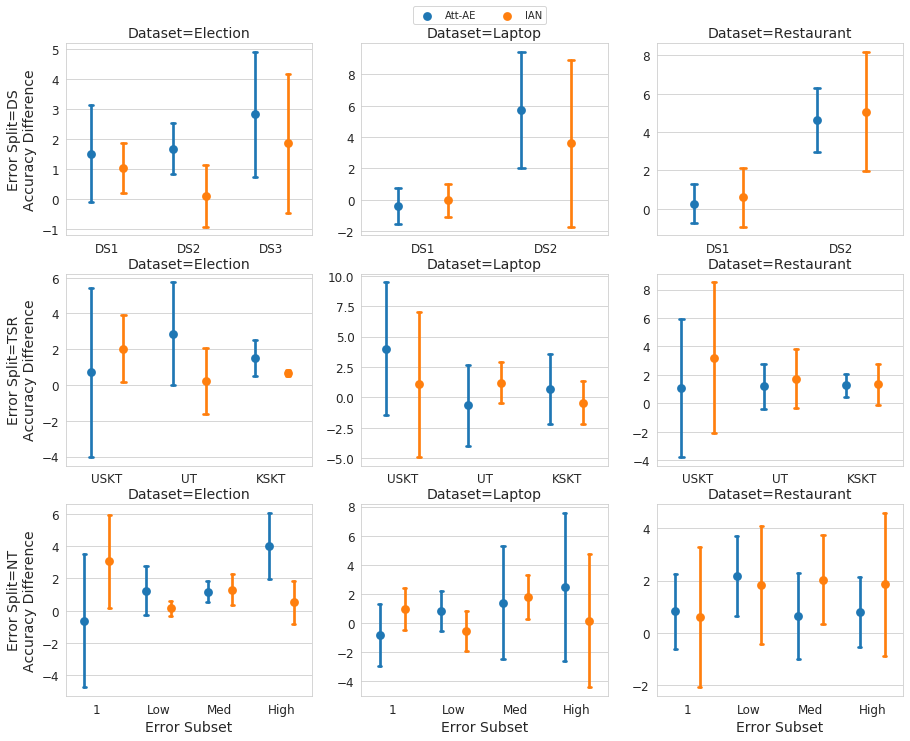
\includegraphics[scale=0.32]{images/augmentation/methods_performance/Position_Encoding/position_split_difference_test_results.png}
    \caption{Test split results. Columns represent different datasets, rows different error splits. Each plot represents the differences between the position and baseline models for the Accuracy metric on the given error subset.}
    \label{fig:aug_position_split_difference_test_results}
\end{figure}

\begin{figure}[h!]
    \centering
    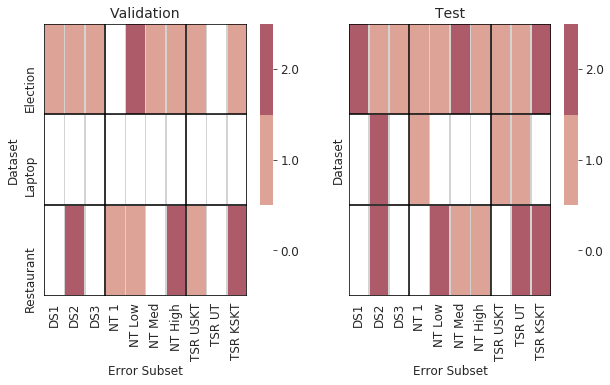
\includegraphics[scale=0.5]{images/augmentation/methods_performance/Position_Encoding/position_dataset_subset_heatmap.png}
    \caption{Heatmaps that represent the number of position models that are statistically significantly better than their baseline equivalents at the 95\% confidence level.}
    \label{fig:aug_position_dataset_subset_heatmap}
\end{figure}

\begin{figure}[h!]
    \centering
    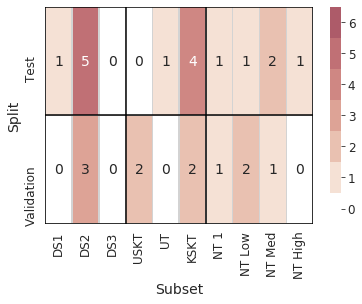
\includegraphics[scale=0.6]{images/augmentation/methods_performance/Position_Encoding/position_combined_subset_heatmap.png}
    \caption{Heatmaps that represent the number of position models that are statistically significantly better than their baseline equivalents across all datasets at the 95\% confidence level. Where the multiple hypothesis tests have been corrected using Bonferroni.}
    \label{fig:aug_position_combined_subset_heatmap}
\end{figure}

As was suggested in the last section \ref{section:aug_baseline} that the \textit{DS} and \textit{TSR} splits should be used when analysing the results, this is the reason why the \textit{TSR} split was included in the figures. From figure \ref{fig:aug_position_combined_subset_heatmap} for the \textit{TSR} split it can be seen that in general the only subset that the position models consistently perform better on is the \textit{KSKT} subset. This is most likely due to the target sentiment relationship modelling improvement, as the \textit{KSKT} subset is the dominate subset within the \textit{TSR} split (see figure \ref{fig:aug_error_analysis_trs}).

\begin{figure}[h!]
    \centering
    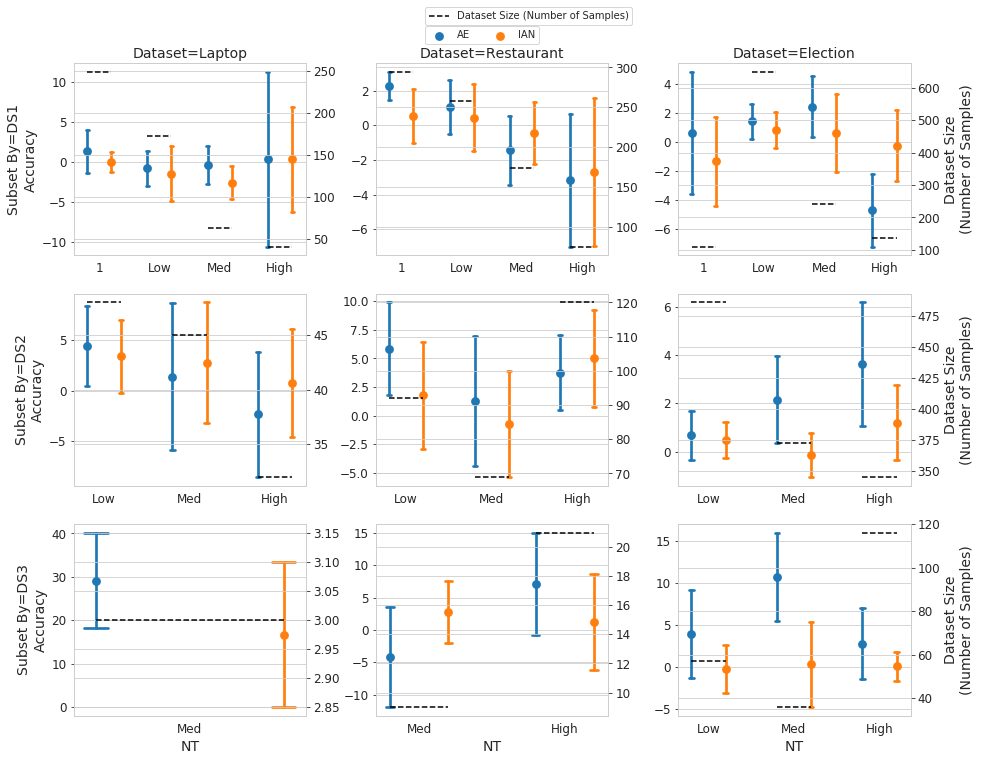
\includegraphics[scale=0.32]{images/augmentation/methods_performance/Position_Encoding/position_DS_NT_validation.png}
    \caption{Validation split results. Columns represent different datasets, rows different \textit{DS} error split subsets. Each plot represents the differences between the position and baseline models for the Accuracy metric on the given error subset.}
    \label{fig:aug_position_DS_NT_validation}
\end{figure}

\begin{figure}[h!]
    \centering
    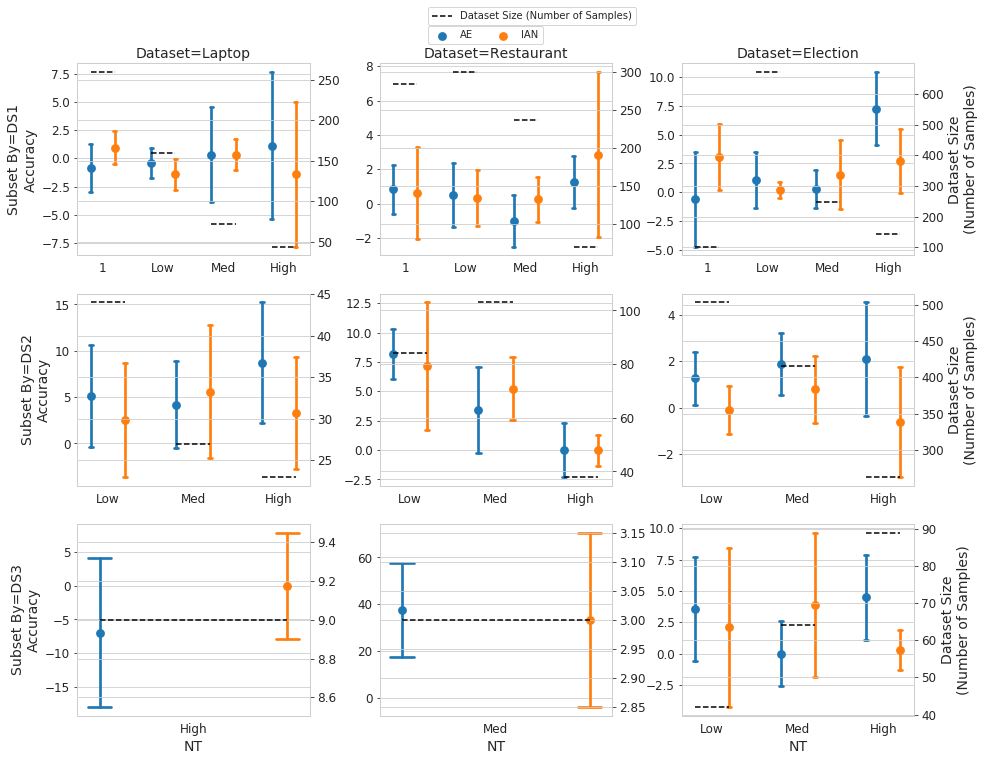
\includegraphics[scale=0.32]{images/augmentation/methods_performance/Position_Encoding/position_DS_NT_test.png}
    \caption{Test split results. Columns represent different datasets, rows different \textit{DS} error split subsets. Each plot represents the differences between the position and baseline models for the Accuracy metric on the given error subset.}
    \label{fig:aug_position_DS_NT_test}
\end{figure}

Lastly, as in the previous work by \citet{he-etal-2018-exploiting}, the way they evaluated the position encoding was through using a similar method to the \textit{NT} error splits. Therefore to show quantitatively that the \textit{NT} splits are not the best way to show that a method improves on target sentiment relationship modelling figure \ref{fig:aug_position_combined_subset_heatmap} finds that only a few models are significantly better across the different \textit{NT} subsets. When any of the \textit{NT} subsets are compared to the $DS_2$ subset none have more significant models. Furthermore, figures \ref{fig:aug_position_DS_NT_validation} and \ref{fig:aug_position_DS_NT_test} show the validation and test split performance difference between the position and baseline models when the data has been first subsetted by the \textit{DS} subsets (rows in the figures) and then further subsetted by the \textit{NT} subsets. From these figures it shows some in-consistencies of which the most of these are in the validation results. The validation results for the Restaurant dataset when subsetted by $DS_1$ show a large negative correlation of which this is most likely due to the baseline model being better a sentiment overfitting on sentences that contain lots of targets. Furthermore on the Laptop test and validation splits for the $DS_1$ subsetted row several of the results mean value is less than $0$ suggesting the baseline model is better in these circumstances. From across the test and validation splits out of all the $DS_1$ subsetted models $29.16\%$($\frac{14}{48}$) perform on average worse than their baseline models compared to $10.4\%$($\frac{5}{48}$) from the $DS_2$ and $DS_3$\footnote{The $DS_3$ subsetted models from the Laptop and Restaurant datasets where not included as they contain very few samples (less than $20$).} subsetted models. This to some degree shows that the \textit{NT} split for the $DS_1$ subsetted data at least is more likely measuring sentiment overfitting than target sentiment relationship modelling, as the baseline model perform competitively. From this it can be seen that when the number of targets does increase the performance of the position models do not always improve the results. Furthermore the \textit{NT} split is more affected by the sentiment factors within the sentence and can be skewed by sentiment overfitting.

\subsection{Conclusion}
This section has found that position encoding does improve TDSA models performance in general. Further it has been shown quantitatively that the theory from the literature on position encoding improving target sentiment relationship modelling \citep{li-etal-2018-hierarchical, he-etal-2018-exploiting} is true through the novel TDSA metrics (\textit{STAC Multi} and \textit{STAC 1}) and existing error split (\textit{DS}). This finding could explain the reason why the \textit{TDLSTM} model performed generally better than the others on the \textit{STAC Multi} metric, and $DS_2$ and $DS_3$ subsets within the baseline results section \ref{section:aug_baseline}. Lastly it has been shown again that the \textit{NT} split is not a useful error split to use due to it being skewed by sentiment overfitting. From this the results that \citet{he-etal-2018-exploiting} presented using a similar error analysis split as \textit{NT} does not quantitatively prove that position encoding does improve target sentiment relationship modelling. Therefore the results presented here are the first quantitative results demonstrating that position encoding does improve target sentiment relationship modelling.

\section{Inter-Target Encoding}
\label{section:aug_inter_target_encoding}
\subsection{Introduction}
The majority of TDSA methods do not explicitly take into account other targets that may occur within the same sentence as the target that it is currently classifying, methods that do take this into account are target-aware. The standard non-target aware methods generally treat the problem as shown in figure \ref{fig:aug_normal_target_modelling}, where for each target (from the three) within the sentence is inputted into the (TDSA) model individually to create a target sentiment aware representation for the target (red/pink square), this representation is then projected down to a vector $\mathbb{R}^{c}$, where $c$ is the number of sentiment classes for prediction. Where as a target-aware model as shown in figure \ref{fig:aug_target_general_modelling} takes all of the targets as input and makes predictions on all targets (three of them in this case) in-affect at the same time, where the model explicitly makes itself aware of all targets within the text through the inter target encoding layer. The Inter target encoding layer was first suggested by \citet{hazarika-etal-2018-modeling}, where they used an LSTM as their Inter Target encoder as shown in figure \ref{fig:aug_target_hazarika_modelling}. As can be seen the LSTM layer is uni-directional thus all targets preceding other targets within the sentence would not be aware of these future targets. This limitation was overcome in \citet{majumder-etal-2018-iarm} where they used a similar network to \citet{hazarika-etal-2018-modeling} but added a memory network on top, of which this memory network performed attention so that each target sentiment representation was aware of all other targets. \citet{zhao2019modeling} instead of using attention and an RNN structure made the targets aware of each other explicitly through a GNN as shown in figure \ref{fig:aug_target_zhao_modelling}. These inter target encoding layer methods is one of two general ways of making a model target aware. The other approach is through regularisation of the attention layer \citep{fan-etal-2018-multi} that is applied to the encoded word representations within the sentence, to make the representations target aware. This form of regularisation was called `Aspect Alignment Loss'\footnote{Aspect here is the same as target.} \citep{fan-etal-2018-multi}, where the intuition behind it was to penalise similar attention weight of targets in the same sentence that contain different sentiment\footnote{Equation 24 shows the Aspect Alignment Loss in \citet{fan-etal-2018-multi}.}. This was to try and force the attention weights of targets that have different sentiment to focus on different words within the sentence. The only other work that has used regularisation to make a model target aware is \citet{hu-etal-2019-constrained}. \citet{hu-etal-2019-constrained} applied a very similar technique to \citet{fan-etal-2018-multi}, however this work was done on the task of aspect based sentiment analysis rather than target\footnote{Aspect based in this thesis is the latent version of target based.}.

\begin{figure*}
        \centering
        \begin{subfigure}[b]{0.475\textwidth}
            \centering
            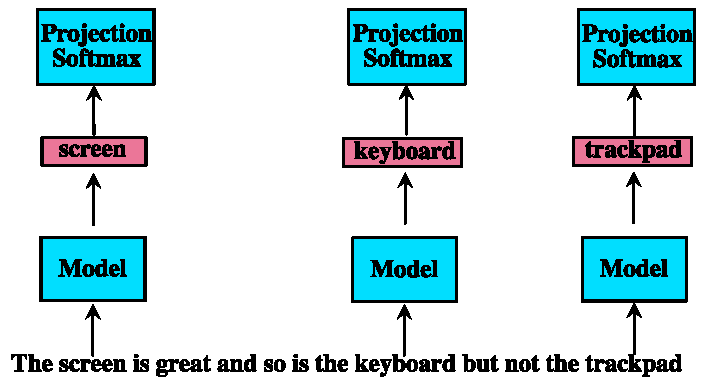
\includegraphics[width=\textwidth]{images/augmentation/methods_performance/Inter_Target/normal.pdf}
            \caption{General non-target aware setup.}    
            \label{fig:aug_normal_target_modelling}
        \end{subfigure}
        \hfill
        \begin{subfigure}[b]{0.475\textwidth}  
            \centering 
            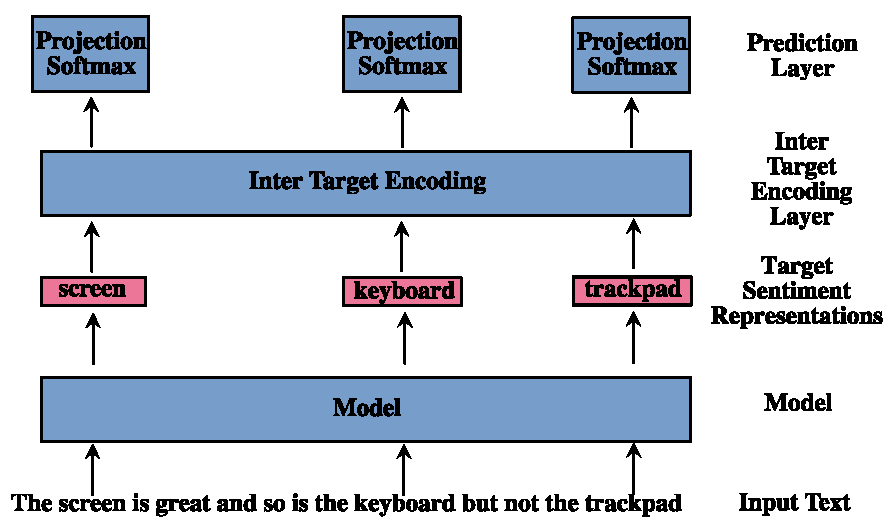
\includegraphics[width=\textwidth]{images/augmentation/methods_performance/Inter_Target/inter_target_encoding.pdf}
            \caption{General target aware setup.}    
            \label{fig:aug_target_general_modelling}
        \end{subfigure}
        \vskip\baselineskip
        \begin{subfigure}[b]{0.475\textwidth}   
            \centering 
            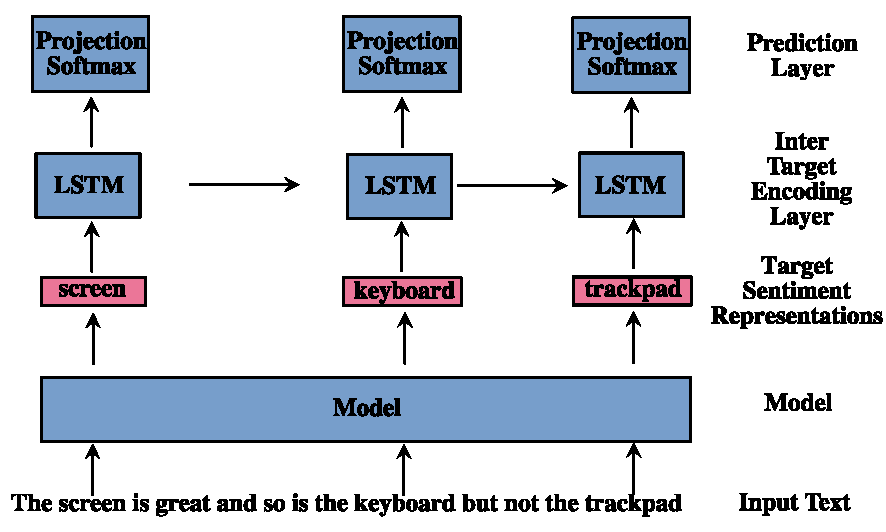
\includegraphics[width=\textwidth]{images/augmentation/methods_performance/Inter_Target/LSTM_Encdoing.pdf}
            \caption{Target aware setup of \citet{hazarika-etal-2018-modeling}.}    
            \label{fig:aug_target_hazarika_modelling}
        \end{subfigure}
        \quad
        \begin{subfigure}[b]{0.475\textwidth}   
            \centering 
            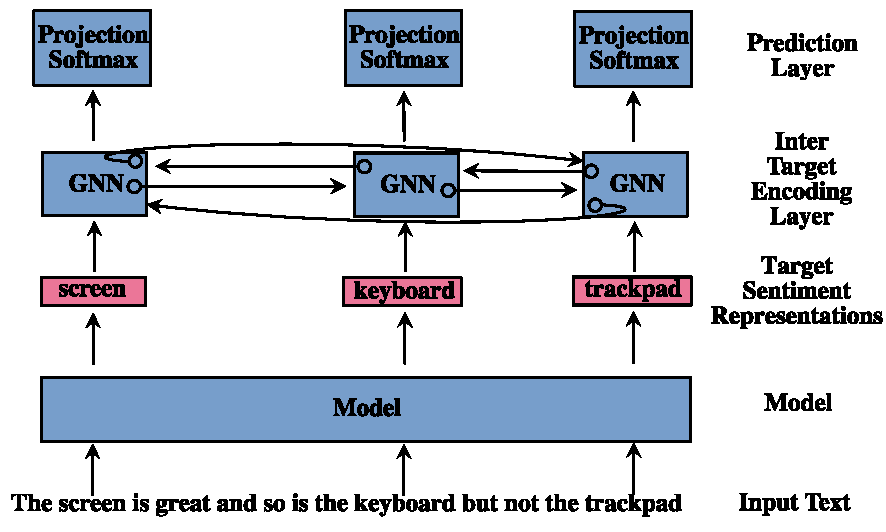
\includegraphics[width=\textwidth]{images/augmentation/methods_performance/Inter_Target/GNN_Encoding.pdf}
            \caption{Target aware setup of \citet{zhao2019modeling}.}    
            \label{fig:aug_target_zhao_modelling}
        \end{subfigure}
        \caption{The first row shows in abstract the difference between non target aware and aware setups. The second row shows more concrete target aware methods.} 
        \label{fig:aug_target_aware_and_non_setups}
\end{figure*}

The main benefit that these papers believe that the inter target encoding layer brings, is the improvement for targets that depend on the sentiment of other targets within the same sentiment. This target interaction was hypothesised within section \ref{section:aug_analysing_the_splits} when describing the different error splits to be quantifiable through the \textit{NT} split. However this was shown not to be the case through the experiments in section \ref{section:aug_baseline}. Thus testing the theory of whether target aware models do perform better on targets that do rely on others cannot be tested here, this would require a specialist corpus as stated earlier in this chapter (section \ref{section:aug_baseline}). Furthermore only one prior work \citep{majumder-etal-2018-iarm} tested this hypothesis more than just qualitatively showing some samples, or dataset statistics on the number of sentences that contain multiple targets. \citet{majumder-etal-2018-iarm} stated the results of their target encoding method on two error subsets of the data, the subset that contains sentence with one target and the sentences that contain more than one target. These two subsets are equivalent to \textit{NT 1-target} and the combination of all of the other \textit{NT} subsets combined respectively. Even though this error analysis \citet{majumder-etal-2018-iarm} performed would not directly test the target interaction hypothesis it was an alternative form of measurement. This alternative form of measurement as shown in section \ref{section:aug_baseline} would not measure target interaction. However in these prior works including the regularisation work \citep{fan-etal-2018-multi}, it was suggested that target aware methods should perform better in sentences that contain multiple targets. Hence the error analysis in \citet{majumder-etal-2018-iarm} was some what a valid choice. This form of coarse measuring of sentences that contain one target and others that contain multiple targets does not measure how good a method is on multiple targets. Rather this measurement is mainly dominated by sentiment factors as shown in section \ref{section:aug_baseline} where sentences that contain one sentiment are easier to classify when they have multiple targets rather than one, even for text classifier methods. Thus knowing that using the number of targets in a sentence cannot state anything about the method in general, the models here will not be evaluated using the same error split as \citet{majumder-etal-2018-iarm}. The models within this section will use the recommended error splits and metrics from section \ref{section:aug_baseline}. These error splits and metrics will inform the community on what the target aware models actually capture more than their baseline equivalents.

The target aware method used in this section is the LSTM approach by \citet{hazarika-etal-2018-modeling} due to the model that is used within the paper to create the target sentiment aware representations being that of the \textit{Att-AE} method. Therefore the \textit{Att-AE} model when enhanced within the inter target encoding will be the same as the model used in \citet{hazarika-etal-2018-modeling}. This will allow direct comparisons with the overall results from \citet{hazarika-etal-2018-modeling}. Furthermore the approach from \citet{hazarika-etal-2018-modeling} was chosen over \citet{majumder-etal-2018-iarm} due to it containing far fewer components within the inter target encoding and the results being only slightly worse\footnote{\citet{hazarika-etal-2018-modeling} (\citet{majumder-etal-2018-iarm}) reported 79\% (80\%) and 72.5\% (73.8\%) accuracy on the Restaurant and Laptop datasets respectively. The reported results was only one accuracy score as they did not run the models multiple times to take into account the random seed/initialisation problem.}. As stated in the introduction the target aware enhancement will be added to all of the TDSA models.



\subsection{Experiments}
As stated in the introduction to this section the \textit{Att-AE} model when enhanced with the LSTM target encoding of \citet{hazarika-etal-2018-modeling} becomes the same model that was used in \citet{hazarika-etal-2018-modeling}. Therefore the first experimental results presented in figure \ref{fig:aug_inter_target_reproducability} shows the single run performance from the reported accuracy scores of \citet{hazarika-etal-2018-modeling}\footnote{The accuracy scores were taken from table 2.} and the distribution of eight scores from the replicated version in this thesis. As can be seen the replicated model does not contain the original model's stated performance within its distribution of scores, thus it failed to replicate the original model. However the replicated model does use the same hyperparameters and components as those stated in \citet{hazarika-etal-2018-modeling}, the only parameter difference is the output dimension of the LSTM that creates a representation for the target words,\footnote{This is LSTM\textsubscript{a} within section 3.1 of \citet{hazarika-etal-2018-modeling}.} in the replicated model it is 300 whereas in the original it is 100. The reason for it being 300 dimension instead of 100 is that the \textit{Att-AE} model is based on two prior works \citet{hazarika-etal-2018-modeling} and \citet{wang-etal-2016-attention} and in \citet{wang-etal-2016-attention} the parameter is 300 not 100\footnote{See the first paragraph of section 4 in \citet{wang-etal-2016-attention}.}. Even though the \textit{Att-AE} model could not replicate that of \citet{hazarika-etal-2018-modeling}, it may not be due to the different parameter decision on the LSTM. As \citet{hazarika-etal-2018-modeling} report similar models that use their inter target encoding layer but have results more similar to those of the replicated model 74.5\% and 73.42\% on the Restaurant dataset and 69.6\% and 63.7\% of the Laptop dataset. As the results reported in \citet{hazarika-etal-2018-modeling} are single run scores, it is hard to determine if the LSTM parameter difference is the reason or the authors had a favourable random seed, as it has been shown for the macro F1 score that these models can range by at 15 F1 points \citep{moss-etal-2019-fiesta}\footnote{See figure 3.}. Even though the results are not replicated, it is still reasonable to compare and contrast the results from the replicated models that use target encoding and the models that do not. As models being compared are replications rather than comparing to the original works results directly. 

\begin{figure}[h!]
    \centering
    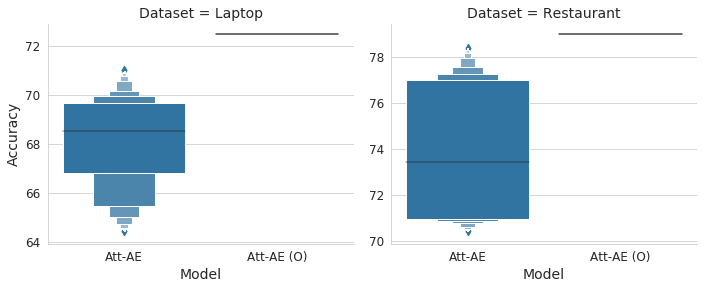
\includegraphics[scale=0.5]{images/augmentation/methods_performance/Inter_Target/inter_target_reproducability.png}
    \caption{Distribution of eight scores and the line represents the mean value, for the original model this line represents their only reported score. Model name with a \textit{(O)} represents the score reported in the original models paper.}
    \label{fig:aug_inter_target_reproducability}
\end{figure}

Figure \ref{fig:aug_overall_inter_target_scores.png} presents the overall results across the different metrics for the inter target encoding models. For easier comparison, figure \ref{fig:aug_overall_difference_inter_target_scores} reports the metric differences between the inter target encoding models and their respective baseline. As can be seen the results are either no better or worse in the majority of cases, only for the \textit{TDLSTM} model for the \textit{STAC 1} metric on the Election dataset are the results better as the standard deviation bars are greater than zero. This shows without performing any statistical tests that, in general, target aware models are not any better than their baseline models. 

\begin{figure}[!h]
    \centering
    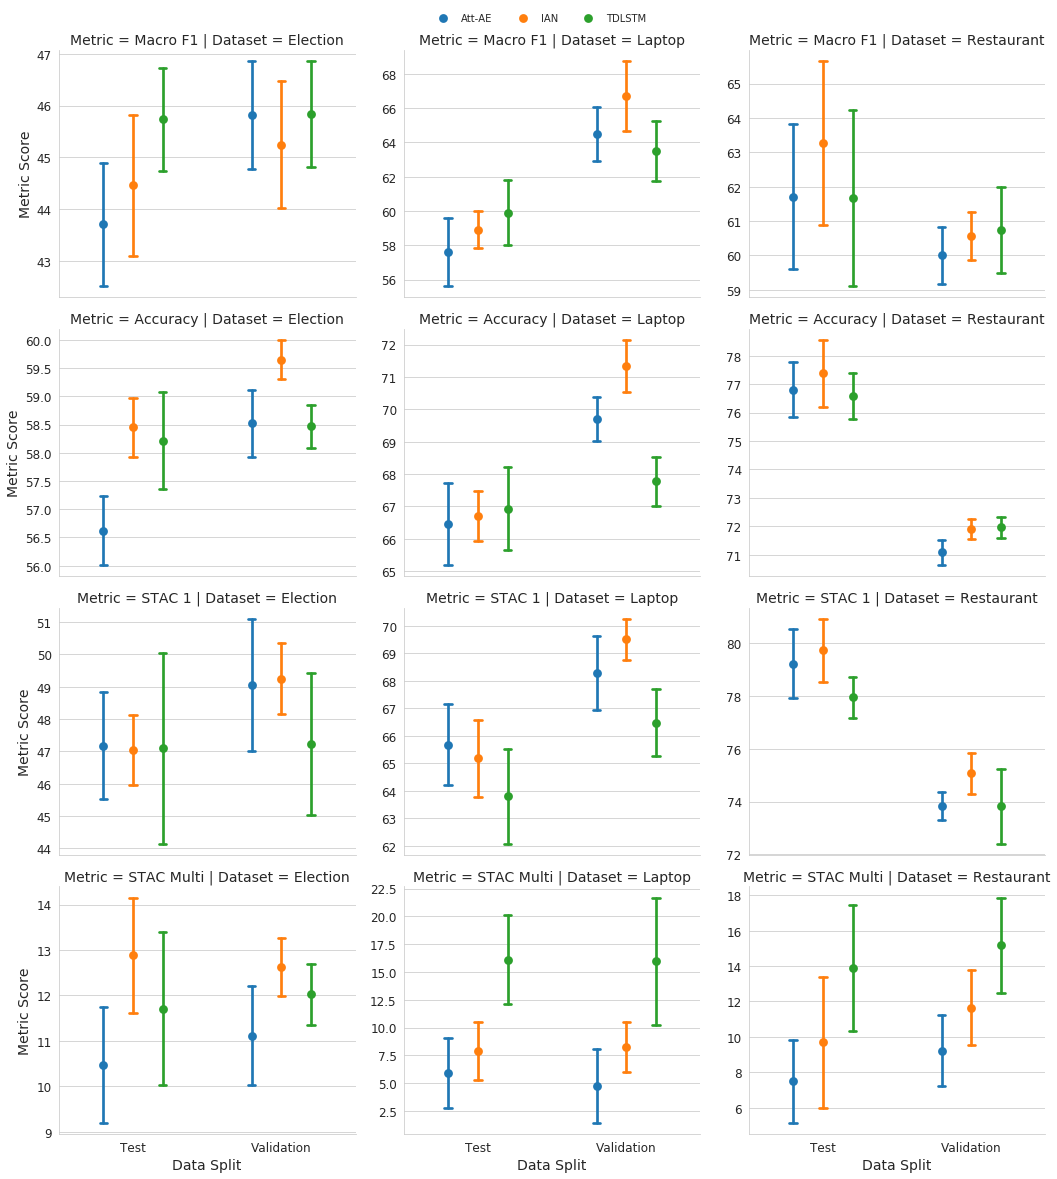
\includegraphics[scale=0.3]{images/augmentation/methods_performance/Inter_Target/overall_inter_target_scores.png}
    \caption{Each plot represents the three target aware enhanced models metric score on the test and validation splits. Columns represent different datasets, rows different metrics.}
    \label{fig:aug_overall_inter_target_scores.png}
\end{figure}
\begin{figure}[!h]
    \centering
    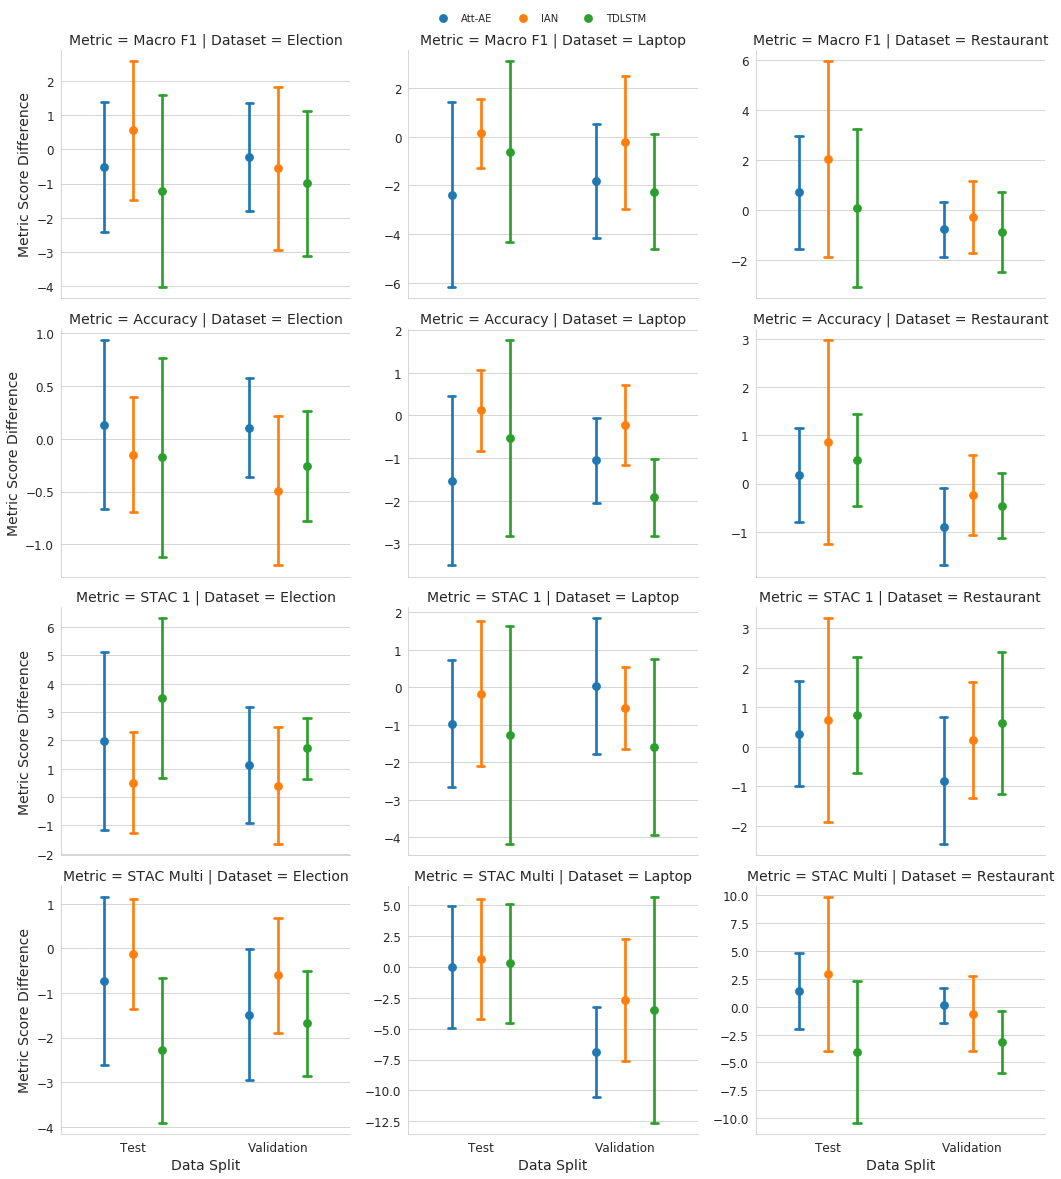
\includegraphics[scale=0.3]{images/augmentation/methods_performance/Inter_Target/overall_difference_inter_target_scores.png}
    \caption{Each plot represents the differences between the target aware and the baseline models for the relevant metric score on the test and validation splits. Columns represent different datasets, rows different metrics.}
    \label{fig:aug_overall_difference_inter_target_scores}
\end{figure}

Thus the heatmaps in figures \ref{fig:aug_dataset_sig_scores_inter_target} \ref{fig:aug_combined_sig_scores_inter_target} show for the left (right) column the number of target aware (baseline) models that are statistically significantly better than their baseline (target aware) models, where the former is not corrected for multiple significance tests whereas the later is using
Bonferroni and is aggregated across datasets. As can be seen the only significant metric difference for the target aware models is on the \textit{STAC 1} metric for the Election dataset, of which when corrected with Bonferroni does not exist. On the other hand the baseline models appear to be better on the accuracy and \textit{STAC Multi} metric across both test and validation splits. This may suggest that for the Election dataset at least that the target aware models are somewhat overfitting to the most frequent sentiment more as they improve the results on the \textit{STAC 1} metric while becoming worse on the \textit{STAC Multi} metric. This would seem intuitive as the model could take advantage of knowing roughly the sentiment of all of the other targets within the sentence due to it's target awareness, and thus take the most likely overall sentiment. However as the number of target aware models that are significantly worse (better) while taking into account multiple tests is low (none) and none for the validation and test splits the assumption of sentiment overfitting cannot be empirically shown. This does show that target aware models from these metrics are not any better and in some cases worse than their baseline equivalent.

\begin{figure}[!h]
    \centering
    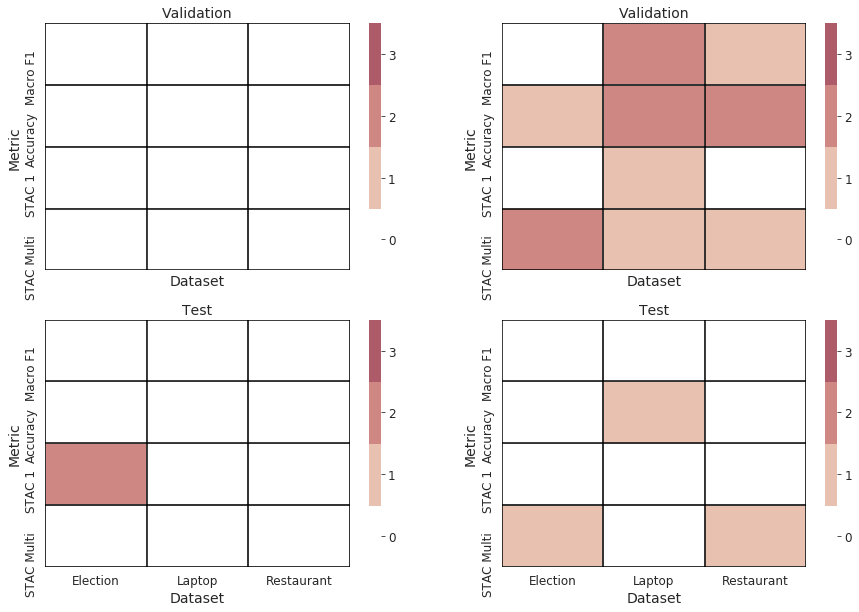
\includegraphics[scale=0.35]{images/augmentation/methods_performance/Inter_Target/dataset_sig_scores_inter_target.png}
    \caption{The left (right) hand side heatmaps represent the number of target aware (baseline) models that are statistically significantly better than their baseline (target aware) equivalents at the 95\% confidence level.}
    \label{fig:aug_dataset_sig_scores_inter_target}
\end{figure}
\begin{figure}[!h]
    \centering
    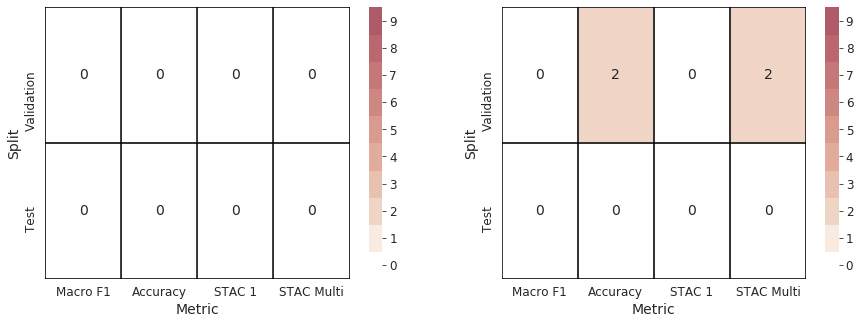
\includegraphics[scale=0.35]{images/augmentation/methods_performance/Inter_Target/combined_sig_scores_inter_target.png}
    \caption{The left (right) hand side heatmaps represent the number of target aware (baseline) models that are statistically significantly better than their baseline (target aware) equivalents across all datasets at the 95\% confidence level. Where the multiple hypothesis tests have been corrected using Bonferroni.}
    \label{fig:aug_combined_sig_scores_inter_target}
\end{figure}

Given these results strongly indicate the target aware models are no better, if not at times worse, than their baseline equivalents, the results comparing target aware to the baseline models across \textit{DS} and \textit{TSR} error splits are shown in figures \ref{fig:aug_inter_target_split_dataset_heatmaps} and \ref{fig:aug_inter_target_split_combined_heatmap} \footnote{The accuracy results for each subset for the test (validation) split are shown in figure \ref{fig:aug_inter_target_encoding_split_overall_test} (\ref{fig:aug_inter_target_encoding_split_overall_validation}). The accuracy difference between the target aware and their associated baseline models are in figures \ref{fig:aug_inter_target_encoding_split_overall_diff_test} and \ref{fig:aug_inter_target_encoding_split_overall_diff_validation} for the test and validation split respectively. These results are within the appendix as they do not show any additional information that the heatmaps in figures do not represent better. They are also within the thesis itself for reproducibility reasons.}. These heatmaps \ref{fig:aug_inter_target_split_dataset_heatmaps} and \ref{fig:aug_inter_target_split_combined_heatmap} show once again that the target aware models are not any better than their baseline equivalents on any subset of any split of any dataset consistently across data splits. Furthermore even though the baseline models are significantly better and consistently better for some subsets of splits as shown in figure \ref{fig:aug_inter_target_split_dataset_heatmaps} when corrected for multiple testing they are not, as shown in figure \ref{fig:aug_inter_target_split_combined_heatmap}. Thus this shows once again the target aware models are no better if not worse in some cases than their baseline equivalents.

\begin{figure}[!h]
    \centering
    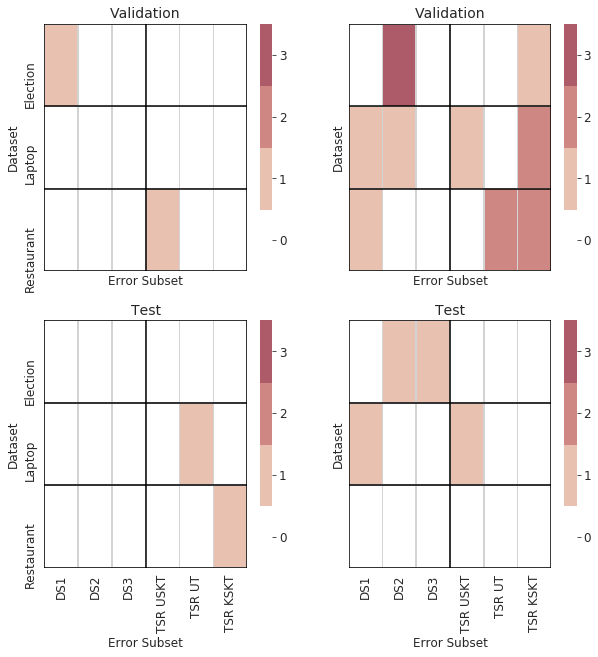
\includegraphics[scale=0.4]{images/augmentation/methods_performance/Inter_Target/inter_target_split_dataset_heatmaps.png}
    \caption{The left (right) hand side heatmaps represent the number of target aware (baseline) models that are statistically significantly better than their baseline (target aware) equivalents at the 95\% confidence level.}
    \label{fig:aug_inter_target_split_dataset_heatmaps}
\end{figure}
\begin{figure}[!h]
    \centering
    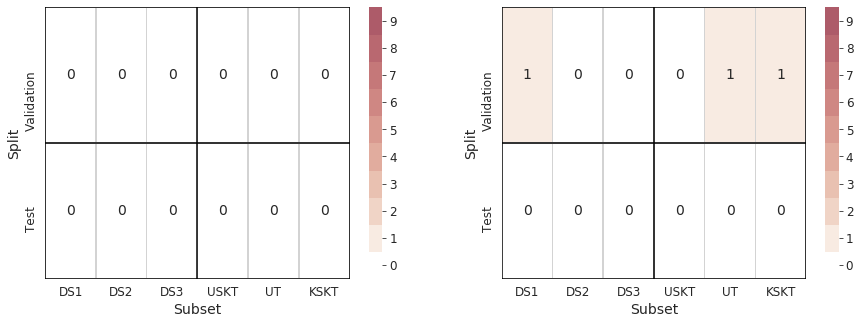
\includegraphics[scale=0.35]{images/augmentation/methods_performance/Inter_Target/inter_target_split_combined_heatmap.png}
    \caption{The left (right) hand side heatmaps represent the number of target aware (baseline) models that are statistically significantly better than their baseline (target aware) equivalents across all datasets at the 95\% confidence level. Where the multiple hypothesis tests have been corrected using Bonferroni.}
    \label{fig:aug_inter_target_split_combined_heatmap}
\end{figure}

\subsection{Conclusion}
To conclude, even though the previous works that incorporated some form of target awareness into their models have shown improvements over their own baseline models \citep{zhao2019modeling, fan-etal-2018-multi}, this has not been shown here. Furthermore it has been shown that on some datasets and some baseline models that they are significantly better than their target aware version. This negative result showing that unlike the previous work here it has been shown that the target aware models are no better than their baseline models could be due to none of the previous works performing rigorous testing of their methods. In all of the previous works none of them perform statistical significant testing nor do they take into account the random seed problem \citep{reimers-gurevych-2017-reporting} which has been shown in chapter \ref{chapter:reproducibility} and \citet{moss-etal-2019-fiesta} to create large error bands on model performances for TDSA. In comparison this work takes both the significance testing and random seeds into account. Even though it was shown that the \textit{Att-AE} model could not replicate the results from the original paper \citep{hazarika-etal-2018-modeling}, it can be concluded here that at least for \citet{hazarika-etal-2018-modeling} inter target encoding method it does not perform any better than not using it. Even though it is stating that opposite of  \citet{hazarika-etal-2018-modeling}, the results here are more rigorously tested and on more models and datasets.

\section{Contextualised Word Representations (CWR)}
\label{section:aug_cwr}
\subsection{Introduction}
% (Looks at point 2 and 3 from the introduction)

%In this section, we are going to look at three different types of Neural Network (NN) systems:
%\begin{enumerate}
%    \item TDLSTM -- A RNN based NN that encodes the target by ensuring the target word(s) are always the last word(s) fed to the RNN from the context. Thus a position based method where the position is encoded through the NN architecture.
%    \item IAN -- Encodes the target into the context via attention.
%    \item InterAE -- Encodes the target into the context by fusing the context and target representations to create a target-context sequence. It further encodes the target into this new target-context sequence by applying attention using the target representation. Then models the other targets within the same context by using an RNN.  
%\end{enumerate}
%Thus to summarise the differences in these TDSA methods; TDLSTM encodes the position of targets through its architecture, IAN encodes the target into the context via attention, and InterAE encodes the target similar to IAN but further models other targets within the same context. Thus using three different types of methods and three different datasets this will ensure that the experimental results and findings to be robust and generalisable. In this subsection the thesis will: 
%\begin{enumerate}
%    \item Review the state of CWR within TDSA and the findings that already exist within the literature. 
%    \item Confirm prior works findings on CWR improving results over non-CWR, as well as the benefits of pre-training CWR.
%    \item How CWR improve TDSA model through novel error analysis.
%\end{enumerate}
  
%\begin{enumerate}
%    \item Are general CWR significantly better than Glove (non-CWR) representations.
%    \item Are domain specific CWR significantly better than general CWR.
%\end{enumerate}
%Furthermore given the better CWR the thesis will explore the differences between CWR and non-CWR with respect to the different splits stated in the error analysis section \ref{section:aug_error_analysis}. Thus showing what gains CWR bring to TDSA and more importantly what is still difficult to classify within TDSA.

%As stated in the introductory section of this chapter \ref{section:aug_introduction}, the three datasets that are used throughout this chapter are the Election, Laptop and Restaurant datasets. However unlike the error analysis section \ref{section:aug_error_analysis}, the standard training split for each of the datasets will be further randomly split into a new training and an additional validation split, and the size of these splits can be seen in table \ref{table:aug_cwr_split_breakdown}. The validation set is required so that the early stopping can be used for all of the NN methods. Furthermore, the validation set would usually be used for more hyper-parameter tuning e.g. finding the best learning rate etc. but due to compute time this is not the case. Instead we selected the most common hyper-parameters from the literature as detailed in table \ref{table:aug_cwr_default_hyperparameters}, it will be stated explicitly within this chapter if these hyperparameters are not used. Lastly all results reported in this section will be results on the test set and all validation results will be reported in the appendix for reproducibility reasons \citep{dodge-etal-2019-show}. However if there is a large difference between the validation and test results this will be mentioned explicitly in this section.

%\begin{table}[ht!]
%    \centering
%    \begin{tabular}{|c|c|c|c|c|}
\hline
        & \multicolumn{4}{c|}{Data Split} \\
\hline
Dataset &          Train &     Validation &           Test &  Total \\
\hline
Election   &  6811 (57.24\%) &  2547 (21.41\%) &  2541 (21.35\%) &  11899 \\
\hline
Laptop     &  1661 (56.29\%) &   652 (22.09\%) &   638 (21.62\%) &   2951 \\
\hline
Restaurant &  2490 (52.73\%) &  1112 (23.55\%) &  1120 (23.72\%) &   4722 \\
\hline
\end{tabular}
%    \caption{Number of samples.}
%    \label{table:aug_cwr_split_breakdown}
%\end{table}

%Due to the splitting of the training dataset, the error analysis split statistics in section \ref{section:aug_error_analysis} will not be identical for the global error splits (\textit{n-shot} and \textit{TRS}) between the train/test and train/validation as they rely on a comparison of train and validation/test. Even though they will not be identical they are relatively similar as shown by table \ref{table:aug_cwr_global_error_diff}. Furthermore as the local splits ($DS_i$, \textit{NT}, and \textit{TSSR}) are only reported for the test set, table \ref{table:aug_cwr_local_error_diff} shows them for the validation and test set showing that they are again relatively similar, thus results should be comparable between validation and test sets.  


The majority of TDSA work so far has only used the standard 840 billion token 300 dimensional \textit{GloVe} vectors \citep{pennington-etal-2014-glove} to initialise word representation within the NN \citep{tang-etal-2016-aspect,tang-etal-2019-progressive}. These non-CWR word vectors in effect transfer semantic and syntactic knowledge of words from the semi-supervised task they were trained from \citep{mikolov2013efficient}. Due to this transferring of knowledge they have been shown to help in multiple NLP settings such as Semantic Role Labelling \citep{collobert2008unified}, Named Entity Recognition, Chunking \citep{turian-etal-2010-word}, and text classification \citep{kim-2014-convolutional}. The word vectors are normally the embedding layer (the first layer) of the NN that is usually trained with a Language Model (LM) type of objective. Thus the data they train from does not require any human annotation. Due to the word vectors coming from this embedding layer the vectors themselves are not contextualised as the NN at this point has not seen any of the other words within the context/text. Therefore the main drawback of non-CWR is that they suffer from word ambiguity \citep{camacho2018word}. 

To overcome this, CWR have been devised which are still trained on a LM objective, but instead of using the embedding layer they either use the second to last layer of the NN \citep{peters-etal-2017-semi}, or a weighted combination of each layers weights which has been shown to be more effective \citep{peters-etal-2018-deep}. These CWR have been shown to outperform non-CWR across a spectrum of NLP tasks by a large margin \citep{liu-etal-2019-linguistic}. The CWR work that has been stated are used in a \textit{feature based} approach where the CWR are fed to a task specific architecture. However, work has also been focused on an alternative approach \textit{fine-tuning} where normally the last layer of the LM NN is replaced with a new task specific layer, and then the whole NN is tuned to the new task \citep{radford2018improving, howard-ruder-2018-universal}. This approach has become very popular since the arrival of BERT \citep{devlin-etal-2019-bert}, due to its impressive performance across multiple tasks compared to other State Of The Art (SOTA) approaches, and its accessibility through the release of its code base\footnote{\url{https://github.com/google-research/bert}}. 

For the interested reader on CWR, there are many different CWR each with subtle differences. These differences are normally based around their learning objective e.g. Bi-LM \citep{peters-etal-2018-deep}, masked LM \citep{devlin-etal-2019-bert}, etc, how they are trained e.g. discriminative fine-tuning \citep{howard-ruder-2018-universal}, model design choices \citep{liu2019roberta}, distillation \citep{tsai-etal-2019-small}, etc if they are multi-lingual \citep{conneau2019cross}, multi task learning with supervised objectives \citep{liu-etal-2019-multi}, for a whole list of papers on CWR see the following GitHub list\footnote{\url{https://github.com/thunlp/PLMpapers}}.

As stated in the introduction section \ref{section:aug_introduction}, previous works have already started to use CWR within TDSA, of which a comprehensive list of these works and metadata details can be seen in table \ref{table:aug_cwr_tdsa_cwr_methods_overview}\footnote{This is most likely already out of date due to the speed that new publications are coming out, and the fact that CWR produce the SOTA results.}. The table clearly shows that a lot of the prior works have tried different architectures: Task Specific Architecture (TSA) and non-TSA\footnote{non-TSA is defined as adding a linear layer on top of the CWR class vector in the case of the BERT model (which is the only CWR model used in prior work).}, fine-tuning or feature based, and pre-training the CWR and not. From this prior work some general insights can be drawn, which will be discussed below.

Pre-training in this thesis is defined as the process of fine-tuning the LM NN that the CWR come from with a separate task and dataset before using the LM NN on the final task, which here is TDSA. A concrete example of pre-training from table \ref{table:aug_cwr_tdsa_cwr_methods_overview}, is pre-training to Yelp and/or Amazon datasets by using an LM objective to fine-tune the BERT\textsubscript{b} LM NN to these dataset, thus making the BERT\textsubscript{b} model more domain specific. Generally one would expect pre-training to improve results as it adapts the CWR to the domain, and this is what both \citet{rietzler2019adapt} and \citet{xu-etal-2019-bert} found. However considering both works use the same pre-training datasets and technique, as well as same CWR and model architecture there is a 2-3\% difference in results. This is most likely due to the lack of pre-training that \citet{xu-etal-2019-bert}\footnote{Used around 1 and 2 million sentences for Laptop and Restaurant domain respectively. This was calculated by multiplying the batch size (16) by the number of training steps.} did not perform, as \citet{rietzler2019adapt} showed that at least 10 million sentences\footnote{These do not have to be the same sentences, as they had 1 million `unique' sentences and 10 million sentence comes from training the model for 10 epochs.} are required before any improvements can be seen for the Laptop domain.

Another insight that can be drawn from the works that use TSAs \citep{zeng2019lcf,zhao2019modeling,song2019attentional,huang-carley-2019-syntax, jiang-etal-2019-challenge} is that using a CWR instead of a non-CWR is always better. This finding is more interesting for the works that do not fine-tune the CWR \citep{zhao2019modeling, huang-carley-2019-syntax} as it shows that by using CWR alone, and not more parameters, results improve over using non-CWR. Furthermore \citet{song2019attentional}, \citet{jiang-etal-2019-challenge}, and \citet{huang-carley-2019-syntax} all found that using a TSA with CWR in a feature based or fine-tuning approach to be better than fine tuning the CWR model with no TSA.

Lastly shown in table \ref{table:aug_cwr_tdsa_non_cwr_methods_overview} are the best performing non-CWR methods\footnote{In both cases they are using \textit{GloVe} vectors and have a TSA.}, of which these are a lot worse in performance compared to any of the CWR methods within table \ref{table:aug_cwr_tdsa_cwr_methods_overview}.

\afterpage{%
    %\clearpage% Flush earlier floats (otherwise order might not be correct)
    \thispagestyle{document}
    \begin{landscape}% Landscape page
            \centering
            \begin{table}
\centering
\begin{tabular}{|c|c|c|c|c|c|c|}
\hline
Authors & Laptop (\%) & Restaurant (\%) & Fine Tuned &  CWR Model & Pre-Trained & TSA \\
\hline
\cite{rietzler2019adapt}   & 80.23 &  \textbf{87.89} &  Yes &  BERT\textsubscript{b} & Yelp, Amazon & No \\
\hline
\cite{zeng2019lcf}   & \textbf{82.45} &  87.14 &  Yes &  BERT\textsubscript{b} & No & Yes \\
\hline
\cite{jiang-etal-2019-challenge}   & - &  85.93 &  Yes &  BERT\textsubscript{b} & No & Yes \\
\hline
\cite{xu-etal-2019-bert}   & 78.07 & 84.95  &  Yes &  BERT\textsubscript{b} & Yelp , Amazon, SQuAD & No \\
\hline
\cite{zhao2019modeling}   & 81.35 &  83.57 &  No &  BERT\textsubscript{b} & No & Yes \\
\hline
\cite{song2019attentional}   & 79.93 &  83.12 &  Yes &  BERT\textsubscript{b} & No & Yes \\
\hline
\cite{huang-carley-2019-syntax}   & 80.1 &  83.0 &  No &  BERT\textsubscript{l} & No & Yes \\
\hline
\multicolumn{7}{|c|}{Bert\textsubscript{b}=BERT base model, Bert\textsubscript{l}=BERT large model \citep{devlin-etal-2019-bert}} \\
\multicolumn{7}{|c|}{TSA=Task Specific Architecture} \\
\hline
\end{tabular}
\caption{Overview of TDSA methods that use CWR}
\label{table:aug_cwr_tdsa_cwr_methods_overview}
\end{table}
    \end{landscape}
    \clearpage% Flush page
}

\begin{table}[!h]
    \centering
    \begin{tabular}{|c|c|c|}
\hline
Authors & Laptop (\%) & Restaurant (\%)\\
\hline
\cite{zhao2019modeling}   & 75.55 &  \textbf{82.95}\\
\hline
\cite{zeng2019lcf}   & \textbf{76.02} &  82.5\\
\hline
\end{tabular}
    \caption{Top performing non-CWR TDSA methods}
    \label{table:aug_cwr_tdsa_non_cwr_methods_overview}
\end{table}

Thus to summarise from this prior work, we can determine that:
\begin{enumerate}
    \item Pre-training is always useful but to be fully utilised it requires fitting on large amounts of pre-training data.
    \item Using a TSA with CWR is better than using a no TSA with CWR.
    \item Using CWR is always better than non-CWR.
\end{enumerate}

%Another interesting difference in the prior works is fine-tuning and Task Specific Architecture (TSA), where no TSA means that only a linear layer is added on top of the CWR model. It would appear based on \citet{zeng2019lcf} that fine-tuning is always better if you have a TSA. However this would contradict the results from \citet{song2019attentional}, which showed for one dataset out of the three evaluated on that the original BERT model fine-tuned was better than there TSA with BERT fine-tuned. Thus this shows some discrepancies between works and that certain TSA are better than others at utilising CWR. Furthermore it has been shown for NER that fine-tuning a BERT type model with a large TSA on top is not optimal \citep{peters-etal-2019-tune}. 

%These works mainly use a non-task specific BERT model \citep{devlin-etal-2019-bert}, where they use a st

The CWR that will be used to investigate the effect it has on the TDSA and text classification methods in this thesis is the ELMo transformer (ET)\footnote{The base ET model can be found here \url{https://allennlp.org/elmo} named as the `Transformer ELMo' model.} as it is quicker for both training and inference than the standard LSTM ELMo, and generally better than a Gated CNN version \citep{peters-etal-2018-dissecting}. Furthermore this is used in the \textit{feature based} manner with a weighted combination of it each layers weights. \textit{Feature based} was chosen over \textit{fine-tuning} as \textit{fine-tuning} adds a large number of parameters to the task specific model, which would therefore mean that we are testing not just CWR but also the affect of adding more parameters. The effect of adding more parameters is thus undesirable and not needed, hence a \textit{feature based} approach was chosen. Furthermore ET was chosen over BERT due to practicalities of training these models at the time of experimentation. Lastly the point of these experiments is to test the differences between CWR and non-CWR rather than differences in CWR for TDSA. As it has been shown in the prior work that domain specific CWR out perform non-domain specific the ET model is pre-trained using an LM task for each domain Laptop, Restaurant and Election. For the Laptop dataset the ET model is pre-trained on the Amazon electronics reviews dataset\footnote{Can be found here \url{http://jmcauley.ucsd.edu/data/amazon/}} \citep{mcauley2015image}, where the ET model is trained on 28,742,985 in domain sentences. The Restaurant dataset uses the 2019 Yelp dataset\footnote{\url{https://www.yelp.com/dataset}} where the ET model is trained on 27,286,698 in domain sentences. Finally the Election dataset unlike the others trains the ET model from scratch on 9,903,000 in domain tweets\footnote{These tweets were collected by scraping Tweets that originate from the current MPs of the time.}. All of the detailed pre-processing, analysis and training of these domain sepcific ET models can be found here \url{https://github.com/apmoore1/language-model}. As \citet{rietzler2019adapt} found that at least 10 million pre-training sentences are required before the CWR models perform any better than their non-domain specific CWR, furthermore the performance of their models saturate after 17 million sentences. This advice from \citet{rietzler2019adapt} has been followed for the Laptop and Restaurant ET models but not the Election ET model. Within the experiment section considering non of the prior work investigated what affect the CWR had on TDSA and text classification methods other than overall Accuracy and macro F1, this will be explored through the recommended metrics and error splits. 

\subsection{Experiments}
To fully report the results figure \ref{fig:aug_overall_cwr_results} shows the different metric scores the CWR TDSA and text classification (\textit{CNN}) models scored on all datasets. The more informative is figure \ref{fig:aug_overall_diff_cwr} which compares the metric scores of the CWR and their respective baseline models. From this figure it can be seen that all of the TDSA models perform better on almost every metric. One the \textit{STAC 1} metric on the Election dataset some of the TDSA models perform worse/no better, which may suggest the models are becoming better at the target sentiment relationship modelling and overfitting less to the most frequent sentiment in the sentence as they improve on the \textit{STAC Multi} metric. Also some of the TDSA models perform worse/no better on the \textit{STAC Multi} metric on the Laptop and Restaurant dataset but perform much better on the \textit{STAC 1} metric suggesting the models are overfitting to the most frequent sentiment in the sentence. This initial analysis suggests to some extent that the CWR increase the performance of the TDSA model by exploiting the artefacts of the datasets. This is shown through the fact that the datasets the contain the least number of $DS_2$ and $DS_3$ sentences Laptop and Restaurant the CWR TDSA models perform a lot better compared to their baseline on the \textit{STAC 1} metric but not the \textit{STAC Multi}. Where as the Election dataset that contains more sentences of $DS_2$ and $DS_3$ combined than $DS_1$ the CWR models perform better compared to their baseline on the \textit{STAC Multi} than the \textit{STAC 1} in general. 

\begin{figure}[!h]
    \centering
    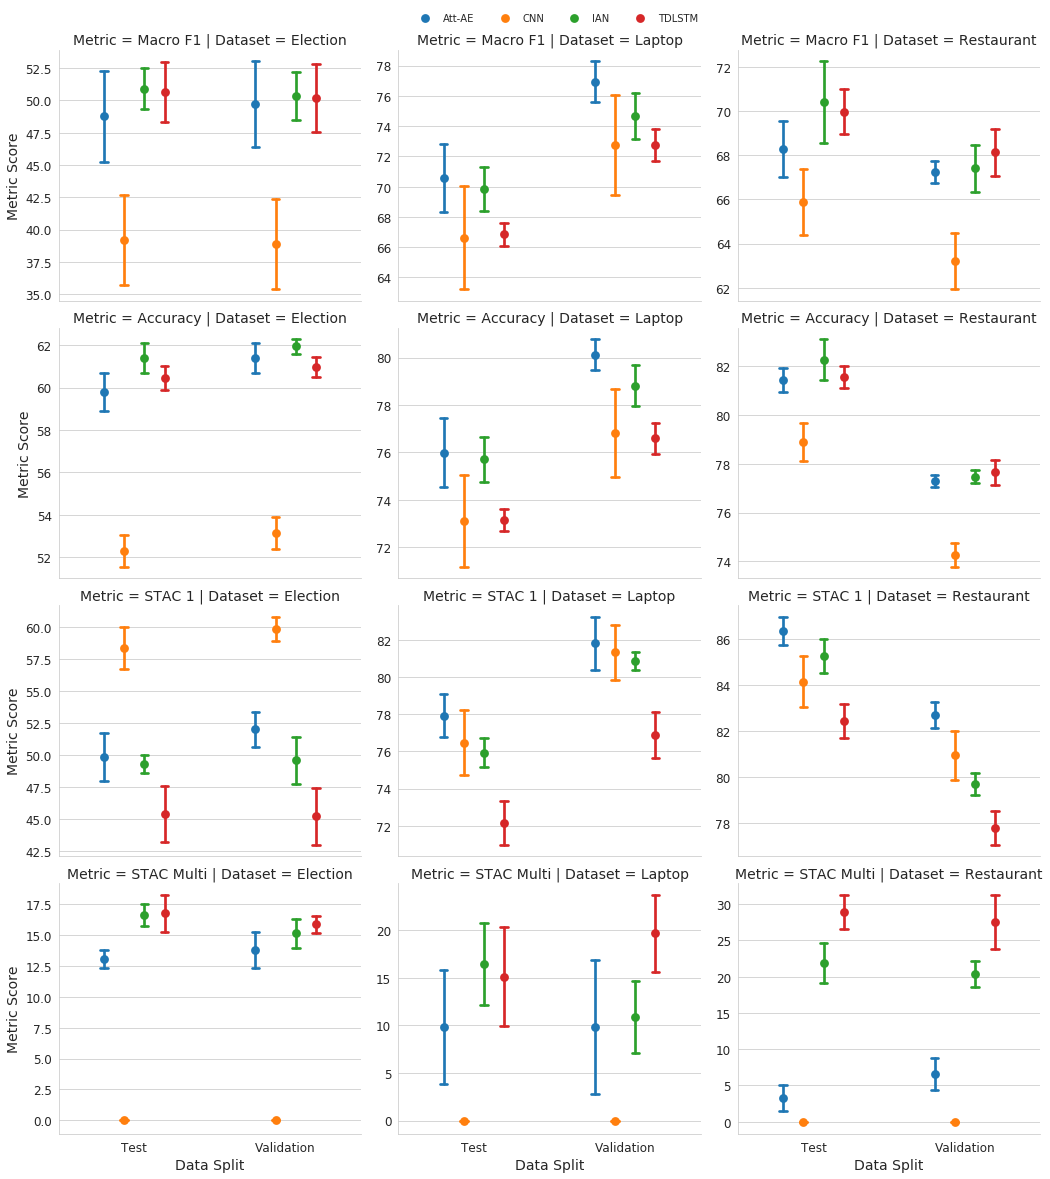
\includegraphics[scale=0.3]{images/augmentation/methods_performance/CWR/overall_cwr_results.png}
    \caption{Each plot represents the CWR models metric score on the test and validation splits. Columns represent different datasets, rows different metrics.}
    \label{fig:aug_overall_cwr_results}
\end{figure}

\begin{figure}[!h]
    \centering
    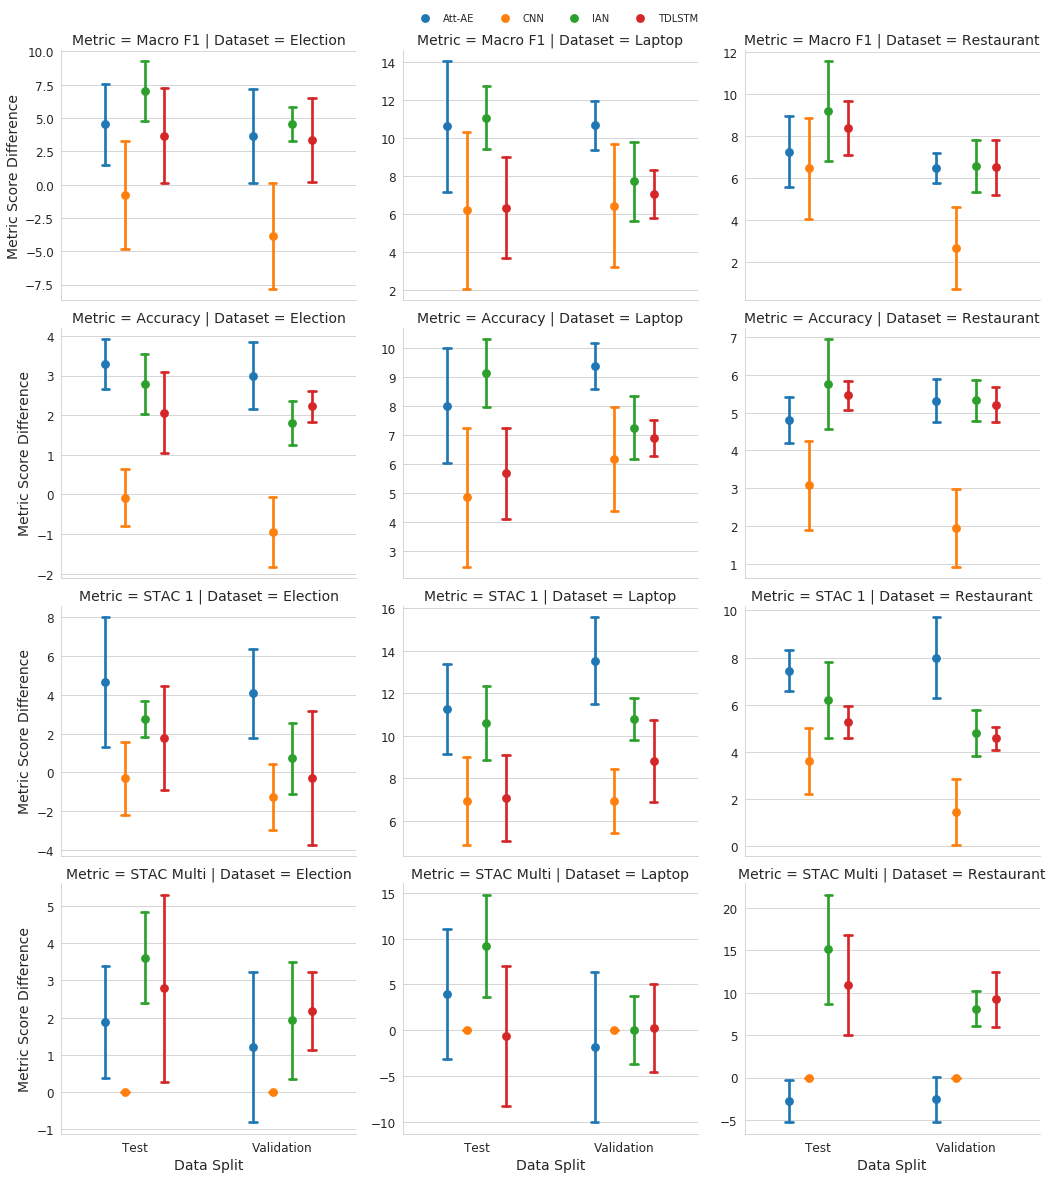
\includegraphics[scale=0.3]{images/augmentation/methods_performance/CWR/overall_diff_cwr.png}
    \caption{Each plot represents the CWR models metric score on the test and validation splits. Columns represent different datasets, rows different metrics.}
    \label{fig:aug_overall_diff_cwr}
\end{figure}

To further investigate this further the heatmaps in figure \ref{fig:aug_cwr_dataset_metric_sig} and \ref{fig:aug_cwr_sig_metric}\footnote{This heatmap does not show the number of baseline models that are significantly better than their CWR model as none were.} show the number of TDSA only CWR models that are statistically significantly better than their baseline, where the former is not correct for multiple significance tests where as the later is using Bonferroni and is aggregated across datasets. It can be seen that for the accuracy metric at least CWR improve over the baseline significantly. Macro F1 when corrected for multiple tests it is not shown as significant as seen in figure \ref{fig:aug_cwr_sig_metric}, this is due to many of the macro F1 significance scores being close to the 95\% confidence limit. Therefore stating that across multiple datasets and models the macro F1 results do not hold to be significant at the 95\% confidence level, showing the importance of correcting for multiple tests. In general and as stated before the CWR models perform significantly better on the \textit{STAC Multi} for the Election dataset but for those that contain far fewer $DS_2$ and $DS_3$ samples this is not true. The \textit{STAC 1} metric is similar to the accuracy in that in almost all cases the CWR are significantly better than their baselines. These significant test some what agree with the initial analysis that the CWR are exploiting the artefacts of the datasets, as they perform generally no better on the \textit{STAC Multi} metric for datasets that contain far fewer $DS_2$ and $DS_3$ samples (Laptop and Restaurant).

\begin{figure}[!h]
    \centering
    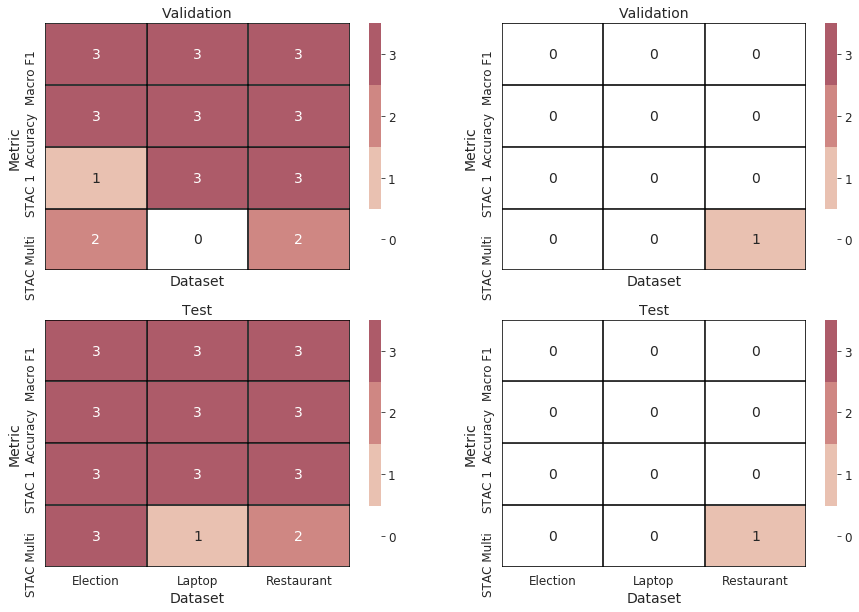
\includegraphics[scale=0.4]{images/augmentation/methods_performance/CWR/cwr_dataset_metric_sig.png}
    \caption{The left (right) hand side heatmaps represent the number of CWR (baseline) models that are statistically significantly better than their baseline (CWR) equivalents at the 95\% confidence level.}
    \label{fig:aug_cwr_dataset_metric_sig}
\end{figure}

\begin{figure}[!h]
    \centering
    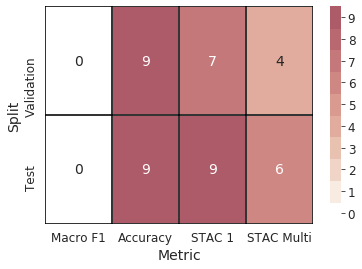
\includegraphics[scale=0.4]{images/augmentation/methods_performance/CWR/cwr_sig_metric.png}
    \caption{The number of CWR models that are statistically significantly better than their baseline equivalents across all datasets at the 95\% confidence level. Where the multiple hypothesis tests have been corrected using Bonferroni.}
    \label{fig:aug_cwr_sig_metric}
\end{figure}

To further investigate whether this initial analysis is true the \textit{DS} error split significance heatmaps can be seen in figures \ref{fig:aug_cwr_dataset_sig_error_splits} and \ref{fig:aug_cwr_combined_sig_error_splits}. Also within those heatmaps are the \textit{TSR} error analysis results, which can be used to study if the CWR improve zero shot target and sentiment relation prediction through the \textit{UT} and \textit{USKT} subsets respectively. The results from the \textit{DS} error splits some what confirm the initial analysis as the laptop validation results for the $DS_2$ subset have no significantly better CWR models. Furthermore out of the nine possible model and dataset combinations only six and five models are significantly better than their baseline for the $DS_2$ subset on the test and validation data splits respectively. This in comparison to almost all CWR models significantly better on the $DS_1$ subset. In comparison to any of the other enhancements this is the first time that the \textit{UT} and \textit{USKT} subsets have improved significantly. This suggests that contextualising the target representations greatly improves the generalisation of them to new targets that are most likely similar to seen targets.

\begin{figure}[!h]
    \centering
    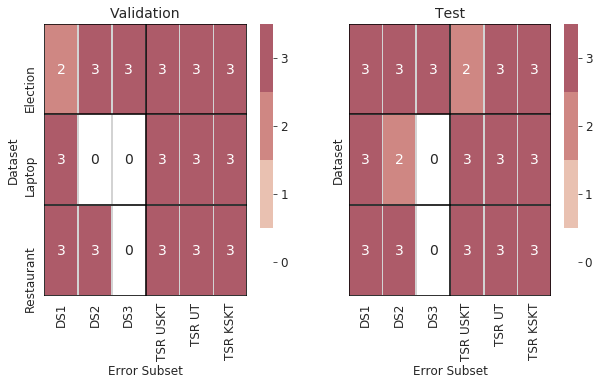
\includegraphics[scale=0.5]{images/augmentation/methods_performance/CWR/cwr_dataset_sig_error_splits.png}
    \caption{The left (right) hand side heatmaps represent the number of CWR (baseline) models that are statistically significantly better than their baseline (CWR) equivalents at the 95\% confidence level.}
    \label{fig:aug_cwr_dataset_sig_error_splits}
\end{figure}

\begin{figure}[!h]
    \centering
    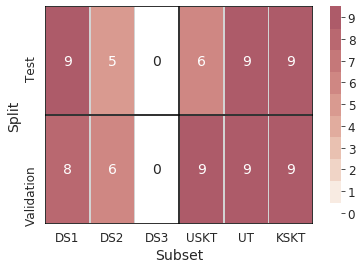
\includegraphics[scale=0.5]{images/augmentation/methods_performance/CWR/cwr_combined_sig_error_splits.png}
    \caption{The number of CWR models that are statistically significantly better than their baseline equivalents across all datasets at the 95\% confidence level. Where the multiple hypothesis tests have been corrected using Bonferroni.}
    \label{fig:aug_cwr_combined_sig_error_splits}
\end{figure}

\subsection{Conclusion}
To conclude, in accordance with the existing literature, it is found that through the general accuracy metric CWR improve TDSA methods significantly compared to using non-CWR (baseline). Unlike the previous work, much greater emphasis has been placed on finding for the first time how CWR improve TDSA models. It has been shown here that the CWR significantly improve the performance of samples that contain unknown targets (\textit{UT}) or unknown sentiment relationship (\textit{USKT}). Thus suggesting that CWR model will perform better in the real world or low resource setting where a lot of the targets or sentiment relationships are not known. It was also found that the macro F1 scores for the CWR are significantly better than their non-CWR but when correcting for multiple tests was not found to be true. Suggesting that creating methods that improve the in-balanced label distribution in these datasets is a fruitful future direction. The CWR would appear to only improve significantly for the \textit{STAC Multi} metric and $DS_2$ subsets when the dataset contains more $DS_2$ and $DS_3$ samples like the Election dataset, improving the target sentiment relationship modelling for those TDSA models. Where as the CWR would almost always improve the \textit{STAC 1} metric and accuracy on the $DS_1$ subset, this suggesting that in some cases the CWR maybe overfitting to the most frequent sentiment in the sentence. Lastly unlike the previous CWR works the overall accuracy results are somewhat lower. This could be due to the fact that a different CWR model was used, ET instead of BERT. Where BERT\textsubscript{b}, even though it contains a similar transformer architecture, it has 12 transformer layers compared to ET's 6. Even though the number of layers this may not be significant, it has been shown for cross lingual performance in Natural Language Inference to be of great importance \citep{wang2019cross} \footnote{See table 4. Depth in table 4 is the same as layers.}. 

\section{Conclusion}
The research question that this chapter was attempting to answer is `How can TDSA methods be measured quantitatively?'. To investigate this, section \ref{section:aug_error_analysis} reviewed the prior work in error analysis splits within TDSA. From this literature review, several existing error splits were found \textit{DS} which measured target sentiment relationship modelling, \textit{NT} measuring target interaction, and \textit{n-shot} measuring generalisation to unknown targets. From this literature review, two novel error splits were created \textit{TSSR} that measured target sentiment overfitting to the most frequent sentiment in a sentence and \textit{TSR} measuring generalisation to unknown sentiment relationships and targets. These existing error splits were rigorously tested in section \ref{section:aug_baseline} across three TDSA methods and a text classification method to ensure they were measuring what was hypothesised. From this \textit{NT} error split was removed due to it not measuring target interaction but rather the sentiment factors \textit{DS}. \textit{TSSR} was dropped due to it not measuring target sentiment overfitting without a text classification model and the \textit{DS} split. Lastly the \textit{n-shot} split was removed as when the value of \textit{n} increased it was expected the accuracy should increase as well or at the least not drop, which was not always true. Thus the \textit{TSR} split which measured both unknown targets and sentiment relationships was recommended as a better replacement to \textit{n-shot}. The findings from reviewing the \textit{NT} split bring the recommendation that the only way to investigate target interaction is through an annotated corpus with this explicitly annotated. A novel TDSA metric is created \textit{STAC Multi} and \textit{STAC 1} which when used together can be used to evaluate sentiment overfitting to the most frequent sentiment in the sentence. Furthermore \textit{STAC Multi} metric can be seen as a coarse grained version of the \textit{DS} error split as they both measure target sentiment relationship modelling, but \textit{STAC Multi} cannot be influenced by sentiment overfitting to the most frequent sentiment in the sentence. Thus from section \ref{section:aug_baseline} the error splits have been reduced to those that match there hypothesises and a new novel metric has been created to over come short comings from the error splits. These recommended error splits and novel metrics are then evaluated in three different TDSA model enhancements position encoding, inter target encoding, and CWR. 

From these three investigations the position encoding showed successfully that the original hypothesis that adding position information does improve target sentiment relationship modelling, due to the position models significant improvements on the \textit{STAC Multi} metric and $DS_2$ subset. Negative results were found for the inter target encoding experiments as all results showed that the baseline models were no worse if not at times better than their inter target encoded enhanced models. Furthermore the original hypothesis that inter target encoding was supposed to improve the model target interaction could not be measured using any error split or metric. From this and the findings of the \textit{NT} split, it is recommended for future work to create a dataset that contains samples that can only be predicted through target interaction so that such a phenomena can be measured. Lastly testing on the CWR where the main hypothesis from the previous work was that the models generally improved as shown through either the accuracy or macro F1 score was confirmed in this thesis. Furthermore the results from the error splits and novel metrics showed for the first time that they significantly improve results for unknown targets (\textit{UT}) and unknown sentiment relationships (\textit{USKT}). This result was not found in any of the other model enhancements. It was also shown that in general they improve target sentiment relationship modelling through the results of \textit{STAC Multi} and $DS_2$. However these results were more convincing on the Election dataset that contained more $DS_2$ and $DS_3$ samples whereas it appeared that the CWR might be overfitting to the overall sentiment in the sentence for datasets that contain less $DS_2$ and $DS_3$ samples (Laptop and Restaurant). These three model investigations to a large extent successfully showed the use of these error splits and in the position encoding investigation how they can match the original hypothesis of why position information is important. Thus as all of the error splits and new metrics are quantitative this answers the original research question of `How can TDSA methods be measured quantitatively?'. This does not mean that new error splits will not be useful.

In comparison to previous works, this chapter has systematically evaluated multiple TDSA models across multiple datasets, multiple random seeds, and model enhancements evaluating using the appropriate statistical tests. Potentially due to this empirical rigour it has shown negative results with respect to inter target encoding, which is the opposite of what the original work found \citep{hazarika-etal-2018-modeling}, which is believed due to the original work not reporting results across multiple random seeds. Other future works have been suggested due to the findings in this chapter, such as exploring whether better modelling target representations so that they better reflect latent aspects would improve results for \textit{UT} error subset. Furthermore if increasing the number of $DS_2$ and $DS_3$ samples could create models that are better at target sentiment relationship modelling without affecting the $DS_1$ samples. Lastly it was shown that the \textit{STAC Multi} metric is by far the worse performing metric and more so than any error subset, this therefore shows that this metric is what future researchers need to focus on.  
%, and the differences are subtle e.g. learning objective and size of model.

%when comparing CWR and non-CWR, the frequently used 300 dimension Glove vectors will be 

%In more recent work pioneered by the BERT model instead of using the outputs from these LM NN to create CWR to be inputted into a task specific network, the LM NN is fined tuned to the task. The fine tune   

%trained with a Language Model (LM) type of objective, thus the data they train from does not require any human annotated data.  for instance Skip-Gram  Even though these word vectors have been shown to help in multiple different NLP settings; Semantic Role Labelling \citep{collobert2008unified}, Named Entity Recognition and Chunking \citep{turian-etal-2010-word}, text classification they fundamentally suffer from word ambiguity/polysemy \citep{peters-etal-2017-semi}. Motivated by this drawback CWR have come about. CWR unlike the non-CWR use either the entire output of 

%These word vectors are non-CWR therefore they are affected by word ambiguity/polysemy \citep{peters-etal-2017-semi}. Motivated by this drawback, CWR have come about, which are multi-layer NN where the layers can be either CNN \citep{peters-etal-2017-semi}, RNN (ELMO), or transformer (BERT) based. The main objective for CWR is similar to that of the non-CWR, in non-CWR the popular objectives are CBOW, Skip-Gram  

